%\section{Detecting Numerical Bug}
\section{Evaluation}
\label{evaluation}
\begin{table*}[t]
  \centering
  % \resizebox{\textwidth}{!}
  {
  \renewcommand{\arraystretch}{1.0}
  % \scalebox{0.8}
  % {
 
 \begin{tabular}{ll|c|c|c|c|c|cc|c}
    \toprule
    \multicolumn{1}{l}{\multirow{2}[2]{*}{Method}} & \multirow{2}[2]{*}{LLM} & \#Vis. & Training & Inference & MMMU & \multirow{2}[2]{*}{MME~\cite{fu2024mmecomprehensiveevaluationbenchmark}} & \multicolumn{2}{c|}{MMBench~\cite{liu2024mmbenchmultimodalmodelallaround}} & SEED~\cite{li2023seedbenchbenchmarkingmultimodalllms} \\
          &       & Tok. & Data$\downarrow$ & TFLOPs$\downarrow$ & VAL~\cite{yue2024mmmumassivemultidisciplinemultimodal} &       & EN & CN & Image \\
    \midrule
    BLIP-2 & Vicuna-7B & 32    & 129M  & 1.25  & -     & 1293.8 & -     & -     & - \\
    InstructBLIP & Vicuna-7B & 32    & 130M  & 1.25  & 30.6  & 1137.1 & 36.0  & 23.7  & 58.8 \\
    MiniGPT-4 & Vicuna-7B & 32    & 517k  & 1.25  & 23.6  & 770.6 & 32.7  & 11.9  & 31.4 \\
    MiniGPT-v2 & Llama2-7B & 256   & 326M   & 4.20  & 25.0  & 708.4 & 24.3  & -     & 29.4 \\
    Otter & Llama-7B & 64    & 2.1B  & 1.67  & -     & 1292.3 & 48.3  & -     & 35.2 \\
    Shikra & Vicuna-7B & 256   & 6.1M  & 4.20  & -     & -     & 58.8  & -     & - \\
    IDEFICS & Llama-7B & 64    & 354M  & 1.67  & 18.4  & 942.0  & 48.2  & 25.2  & 44.5 \\
    IDEFICS & Llama-65B & 64    & 354M  & 16.62 & -     & 1244.9     & 54.5  & 38.1  & 53.2 \\
    Qwen-VL-Chat & Qwen-7B & 256   & 1.4B  & 4.20  & 36.0  & 1435.2 & 60.6  & 56.7  & 65.4 \\
    LLaVA-1.5 & Vicuna-7B & 576   & 1.2M  & 8.53  & 35.7  & \textbf{1510.7} & 64.3  & 58.3  & \textbf{66.1} \\
    \rowcolor{cyan!20} SAISA (Ours) & Vicuna-7B & 576   & 1.2M  & 2.86  & \textbf{36.9} & 1461.9 & \textbf{65.7} & \textbf{59.0} & 64.5 \\
    \bottomrule
    \end{tabular}%
    }
  % }
  \caption{\textbf{Performance on comprehensive benchmarks for instruction-following MLLMs.}
  \#Vis. Tok.: the number of visual tokens involved in a single image.
  \#Training Data: accumulated multimodal pre-training and fine-tuning data volume.
  Inference TFLOPs: the computational cost of processing a single image when the number of text tokens is 64.
  $\downarrow$: a lower value in these columns is better.
    SAISA achieves the best performance on 3/5 benchmarks, while reducing inference TFLOPs by 66\% compared to LLaVA-1.5.
  }
  \label{tab:mllms}%
\end{table*}

We conducted all our experiments on a server equipped with an Intel Xeon E5-26 CPU and eight NVIDIA 1080 Ti GPUs. We set up 0.3 and 0.2 as the threshold based on our validation score on detecting out-of-scope inputs for vulnerability detection and defect prediction tasks, respectively, on all subjects. We set up maximum iteration to three and different crossover rates (i.e., 0.16, 0.33, 0.66, and 1)  when applying sequences of transformation operators on each subject matter described in Section~\ref{evaluation}.

%We set up 0.3 and 0.2 as the threshold based on our validity score on detecting out-of-scope inputs for vulnerability detection and defect prediction tasks respectively on all subjects. We set up maximum iteration to three, and crossover rate of 0.5 when applying program transformations on each subject matter. 

\subsection{Research Questions }
%We aim to answer the following research questions in the next section:

\noindent\textbf{RQ1. Overall Performance: }What is the overall performance of CodeImprove?

\noindent\textbf{RQ2. Input Validation: } How effective is the out-of-scope program data detection? 

\noindent\textbf{RQ3. Input Adaptation: } How effective to convert out-of-scope data to become in-scope data?

\noindent\textbf{RQ4. Setting Sensitivity: }
How sensitive is CodeImprove's performance under different experimental setups? 

%%\noindent\textcolor{blue}{\textbf{RQ5. Submodel Decomposition: }How effective is the submodel generation in detecting out-of-scope data detection?}

%\textbf{RQ3. Layer Selection:} Does the choice of layers for selection have an impact on out-of-scope data detection?
\noindent\textbf{RQ5. Semantic Preserving:} Does program transformations of CodeImprove preserve semantics?


%\textbf{RQ5. Transformation:} How effective are the program transformations on out-of-scope data?

\noindent\textbf{RQ6. Runtime Overhead:} What is the overhead of CodeImprove in adapting a program to DL models?

%\textbf{RQ6. Controlling Factors: } What factors contribute to the impact on the performance of DL models?





%\textbf{RQ2.} What is the accuracy of the model with transformed programs?


\subsection{Subjects}
\label{subjects}
\subsubsection{Datasets and Tasks}
CodeImprove is evaluated on two code-based classification tasks: vulnerability prediction with devign dataset ~\cite{zhou2019devign}, and defect prediction with codeChef dataset~\cite{phan2017conv}.~\textcolor{blue}{Although this study used two datasets, CodeImprove applies to all code model-based tasks, with plans for broader future evaluations.}

%{While these two datasets were selected for this study, CodeImprove is applicable to all code model-based tasks, and we plan to evaluate CodeImprove on a broader range of tasks in the future.}

%To evaluate CodeImprove, we consider two code-based classification tasks and two associated datasets (i.e., vulnerability prediction with devign dataset ~\cite{zhou2019devign}, and defect prediction with codeChef dataset~\cite{phan2017conv}).   


%The statistics of datasets are shown at the first four columns in Table~\ref{table:datasets}, each of which represents the task, the number of classes for the classification task, the class names, the number of samples in each class, the number of inputs in the training/validation/test set, and the programming language for the inputs. 

For \textbf{vulnerability detection}, the Devign dataset\cite{zhou2019devign} consists of 27,318 functions extracted from FFmpeg and Qemu open-source C projects. The functions are labeled as containing vulnerabilities or being clean, with 14,858 vulnerable and 12,460 clean samples. The dataset is split into train/validation/test sets with sizes 21,854/2,732/2,732.

For \textbf{defect prediction}, the CodeChef dataset includes 33,822 C/C++ functions from the CodeChef platform~\cite{phan2017conv}. \textcolor{blue}{Samples are labeled with categories such as}
%Samples are labeled as having 
no defect, wrong output, timeout error, or runtime error, with 11,362 no defect, 13,656 wrong output, 5,101 timeout error, and 3,703 runtime error samples. The dataset is divided into train/validation/test sets with sizes 21,647/5,411/6,764.








%The task of \textbf{vulnerability detection} aims to predict whether a given code snippet contains vulnerabilities. We use the dataset that was prepared by \cite{zhou2019devign}. The dataset is extracted from two popular open-sourced C projects: FFmpeg and Qemu, consisting of 27,318 functions that are labeled as either containing vulnerabilities or clean. The number of vulnerable samples are 14858 and clean samples are 12460. The dataset consists of 21854/2732/2732 as train/validation/test samples. The task of \textbf{defect prediction} aims to predict whether a given code snippet is defective and its defect type. We use the CodeChef dataset that was prepared by ~\cite{phan2017conv}. The dataset is extracted from the CodeChef platform that contains 33822 C/C++ functions that are labeled as no defect, wrong output, timeout, or runtime error. The dataset consists of 11362 no defect samples, 13656 wrong output samples, 5101 timeout error samples, and 3703 runtime error samples. The dataset consists of 21647/5411/6764 as train/valid/test samples. 


%This dataset is included as part of the CodeXGLUE benchmark~\cite{} that has been used to investigate the effectiveness of CodeBERT for vulnerability prediction. CodeXGLUE divides the dataset into training, development and test set that we reuse in this study. 
 


%\begin{table*}[ht]
    \footnotesize
    \centering
    \renewcommand{\arraystretch}{1.1} % Adjusts the row spacing
    \resizebox{16cm}{!} 
    { 
    \begin{tblr}{hline{1,2,Z} = 0.8pt, hline{3-Y} = 0.2pt,
                 colspec = {Q[l,m, 13em] Q[l,m, 6em] Q[c,m, 8em] Q[c,m, 5em] Q[l,m, 14em]},
                 colsep  = 4pt,
                 row{1}  = {0.4cm, font=\bfseries, bg=gray!30},
                 row{2-Z} = {0.2cm},
                 }
\textbf{Dataset}       & \textbf{Table Source} & \textbf{\# Tables / Statements} & \textbf{\# Words / Statement} & \textbf{Explicit Control}\\ 
\SetCell[c=5]{c} \textit{Single-sentence Table-to-Text}\\
ToTTo \cite{parikh2020tottocontrolledtabletotextgeneration}   & Wikipedia        & 83,141 / 83,141                  & 17.4                          & Table region      \\
LOGICNLG \cite{chen2020logicalnaturallanguagegeneration} & Wikipedia        & 7,392 / 36,960                  & 14.2                          & Table regions      \\ 
HiTab \cite{cheng-etal-2022-hitab}   & Statistics web   & 3,597 / 10,672                  & 16.4                          & Table regions \& reasoning operator \\ 
\SetCell[c=5]{c} \textit{Generic Table Summarization}\\
ROTOWIRE \cite{wiseman2017challengesdatatodocumentgeneration} & NBA games      & 4,953 / 4,953                   & 337.1                         & \textbf{\textit{X}}                   \\
SciGen \cite{moosavi2021scigen} & Sci-Paper      & 1,338 / 1,338                   & 116.0                         & \textbf{\textit{X}}                   \\
NumericNLG \cite{suadaa-etal-2021-towards} & Sci-Paper   & 1,355 / 1,355                   & 94.2                          & \textbf{\textit{X}}                    \\
\SetCell[c=5]{c} \textit{Table Question Answering}\\
FeTaQA \cite{nan2021fetaqafreeformtablequestion}     & Wikipedia      & 10,330 / 10,330                 & 18.9                          & Queries rewritten from ToTTo \\
\SetCell[c=5]{c} \textit{Query-Focused Table Summarization}\\
QTSumm \cite{zhao2023qtsummqueryfocusedsummarizationtabular}                        & Wikipedia      & 2,934 / 7,111                   & 68.0                          & Queries from real-world scenarios\\ 
\textbf{eC-Tab2Text} (\textit{ours})                           & e-Commerce products      & 1,452 / 3,354                   & 56.61                          & Queries from e-commerce products\\
    \end{tblr}
    }
\caption{Comparison between \textbf{eC-Tab2Text} (\textit{ours}) and existing table-to-text generation datasets. Statements and queries are used interchangeably. Our dataset specifically comprises tables from the e-commerce domain.}
\label{tab:datasets}
\end{table*}

\subsubsection{Models}
We employed state-of-the-art pre-trained models, namely CodeBERT~\cite{fengCodeBERTPreTrainedModel2020}, RoBERTa~\cite{Liu2019RoBERTa}, and GraphCodeBERT~\cite{guo2021graphcodebert} which have been widely utilized in previous studies~\cite{lu2021codexglue,tian2023code,yang2022natural,carrot}. These models were fine-tuned on our tasks using the corresponding datasets, adhering to the recommended settings proposed in previous literature~\cite{lu2021codexglue}. Hyper-parameters were set to match the original configurations. \textcolor{blue}{CodeImprove is designed for use with all types of code models.} \textcolor{blue}{Our study includes a diverse range of tasks, pre-trained models, and class numbers, ensuring a comprehensive evaluation of CodeImprove's performance.}
%Our study consists of a diverse range of subjects, spanning different tasks, pre-trained models, and class numbers. This diversity ensures a comprehensive evaluation of CodeImprove's performance.


%These models have been used in the existing work that adapts code models~\cite{lu2021codexglue,tian2023code,yang2022natural,carrot}. We fine-tuned these models on the two tasks based on the corresponding datasets respectively, following the settings recommended by the existing work ~\cite{lu2021codexglue}. We set the hyperparameters similar to the original setup. %Table~\ref{table:parameters} shows hyperparameters of each model on each task. For each task, we imply the same hyperparameters for each model. 

%Overall, the subjects used in our study are diverse, involving different tasks, different pre-trained models, and different numbers of classes, It is very helpful to sufficiently evaluate the performance of CodeImprove.


%%We employed state-of-the-art pre-trained models, namely CodeBERT [41], RoBERTa [42], and GraphCodeBERT [9], which have been widely utilized in previous studies that focus on code model adaptation [4], [33], [43], [44]. These models were fine-tuned on our tasks using the corresponding datasets, adhering to the recommended settings outlined in previous literature [4]. Hyperparameters were set to match the original configurations.

%%Our study encompasses a diverse range of subjects, spanning different tasks, pre-trained models, and class numbers. This diversity ensures a comprehensive evaluation of CodeImprove's performance.







%%%%ISSTA \subsection{Baseline Techniques: }
%%%%ISSTA \subsubsection{Techniques employed to evaluate overall performance }

%ISSTA We compared CodeImprove with other search based techniques namely, random search (\textbf{CodeImprove-rand}), Hill climbing algorithm (\textbf{CodeImprove-HC}),and \textcolor{red}{A-star search (\textbf{CodeImprove-A*})}. \textbf{CodeImprove-rand} is designed to apply random transformations until identifying the optimal candidate. \textbf{CodeImprove-HC} is designed based on the princliples of hill climbing algorithm. The search strategy begins with an initial solution (i.e., obtained through a random transformation). Subsequently, it iteratively applies single transformations to this solution while computing the fitness score. If the current solution surpasses the threshold for fitness score, the algorithm terminates, having achieved the optimal solution. 

%%%%ISSTA \subsubsection{Techniques employed to evaluate input validation }We compared CodeImprove's DSMD with the Cross-Layer Dissection (\textbf{CLD})~\cite{wang2020dissector}. Here, we utilized the validity score in DSMD, however employed the similar sub-model generation technique in ~\cite{wang2020dissector}.

%\textbf{CodeImprove-PSO} is designed based on the princliples of particle swarm optimization algorithm. The process begins by defining each particle as a transformation. We initialize a swarm of particles where each particle's position is a generated by applying the transformation. 












%\begin{tikzpicture}[
	font=\footnotesize,
	node distance=0.3cm
	]
	\node[] (P) at (0,0)  {
		\textbf{Parameter:} Key-Gen()
	};
	\node[] (c) [below = 0cm of P] {
		\begin{minipage}{0.8\columnwidth}
			\begin{minted}[fontsize=\footnotesize,escapeinside=@@,autogobble]{coq}
Parameter KeyGen, (PubKey × SecKey).
			\end{minted}
		\end{minipage}
	};
	
	% Package frame and stuff
	\draw[] (c.north west) |- (P.north) -| (c.north east);
	\draw[] (c.north west) |- (P.south) -| (c.north east);
	\draw[] (c.north east) |- (c.south) -| (c.north west);
	
	%%%%%%%%%%%%%%%%%%%%%%%%%%%%%%%%%%%%%%%
	%%%%%%%%%%%%%%% Sign %%%%%%%%%%%%%%%%%%
	%%%%%%%%%%%%%%%%%%%%%%%%%%%%%%%%%%%%%%%
	
	\node[] (P1) [below = 0.7cm of P]  {
		\textbf{Parameter:} Sign(m,sk)
	};
	\node[] (c1) [below = 0cm of P1] {
		\begin{minipage}{0.8\columnwidth}
			\begin{minted}[fontsize=\footnotesize,escapeinside=@@,autogobble]{coq}
Parameter Sign : @$\forall$@ (sk : SecKey) (m : Message), 
  Signature.
			\end{minted}
		\end{minipage}
	};
	
	% Package frame and stuff
	\draw[] (c1.north west) |- (P1.north) -| (c1.north east);
	\draw[] (c1.north west) |- (P1.south) -| (c1.north east);
	\draw[] (c1.north east) |- (c1.south) -| (c1.north west);
	
	%%%%%%%%%%%%%%%%%%%%%%%%%%%%%%%%%%%%%%%
	%%%%%%%%%%%%%%% Verify %%%%%%%%%%%%%%%%
	%%%%%%%%%%%%%%%%%%%%%%%%%%%%%%%%%%%%%%%
	
	\node[] (P2) [below = 1cm of P1]  {
		\textbf{Parameter:} Verify(m,sig,pk)
	};
	\node[] (c2) [below = 0cm of P2] {
		\begin{minipage}{0.8\columnwidth}
			\begin{minted}[fontsize=\footnotesize,escapeinside=@@,autogobble]{coq}
Parameter Ver_sig : @$\forall$@ (pk : PubKey) 
  (sig : Signature) (m : Message), bool.
			\end{minted}
		\end{minipage}
	};
	
	% Package frame and stuff
	\draw[] (c2.north west) |- (P2.north) -| (c2.north east);
	\draw[] (c2.north west) |- (P2.south) -| (c2.north east);
	\draw[] (c2.north east) |- (c2.south) -| (c2.north west);
	
\end{tikzpicture}





\subsection{Evaluation Metrics }

We use a diverse set of metrics to measure CodeImprove’s effectiveness for our six RQs.   

%\textbf{Accuracy:} Accuracy = $\frac{TP+TN}{TP+TN+FP+FN}$. 
The \textbf{accuracy (A)} is the proportion of correctly classified samples out of all samples. %TN represents the number of true negatives and TP + TN + FN + FP represents the number of all samples.
 %\textbf{Precision:} Precision = $\frac{TP}{TP+FP}$. 
The \textbf{precision (P)} is the percentage of correctly predicted positive samples out of all positive predictions. %TP and FP denote the number of true positives and false positives, respectively. 
%\textbf{Recall:} Recall = $\frac{TP}{TP+FN}$. 
The \textbf{recall (R)} measures the percentage of correctly predicted positive samples that were retrieved out of all actual positive samples.  %TP and FN denote the number of true positives and false negatives, respectively.
%\textbf{F1-Score:} F1 = $\frac{2*Precision*Recall}{Precision+Recall}$ = $\frac{2*TP}{2*TP+FP+FN}$. 
The \textbf{F1 score (F1)} is the harmonic mean of precision and recall. 
\textbf{Relative improvement (RI)} quantifies the accuracy improvement relative to the difference between training and test accuracy.

%is measured by the amount of accuracy improved over the difference between training accuracy and test accuracy.

% \textbf{Relative Improvement: }RI = $\frac{\text{New Accuracy} - \text{Orginal Accuracy}}{\text{Training accuracy- Original Accuracy}}*100$

\textbf{ Correction success rate (CSR)}~\cite{tian2023code}
is the ratio of successfully corrected mispredictions to the total identified mispredictions. \textbf{Mis-correction rate (MCR)}~\cite{tian2023code} measures the negative effect caused, which is the ratio of correct predictions changed to mispredictions to the total number of correct predictions in the test set.

%measures the ability to correct mispredictions, which is the ratio of the number of inputs whose mispredictions are successfully corrected to the total number of identified mispredicted inputs. \textbf{Mis-correction rate (MCR)} measures the negative effect caused, which is the ratio of the number of inputs whose correct predictions are changed to mispredictions to the total number of inputs with correct predictions in the test set.

\textbf{ Correction validation rate (CVR)} is the ratio of successfully validated mispredictions to the total possible mispredicted inputs to be validated. \textbf{Mis-correction validation rate (MVR)} is the ratio of correct predictions validated as mispredictions to the total number of correct predictions in the test set. \textbf{AUC} score evaluates the effectiveness of the input validation process. \textbf{Transformations per Second (TPS)} measures the rate of transformations CodeImprove can apply per second. Next, we will describe the results of the experiments.


%%%measures the ability to validate correct mispredictions, which is the ratio of the number of inputs whose mispredictions are successfully validated to the total number of possible mispredicted inputs to be validated. \textbf{Mis-correction validation rate (MVR)} measures the negative effect caused, which is the ratio of the number of inputs whose correct predictions are validated as mispredictions to the total number of inputs with correct predictions in the test set. \textbf{AUC} score to evaluate our effectiveness of input validation process \textbf{AUC} score to evaluate our effectiveness of input validation process. \textbf{Transformations per Second (TPS)} measures the number of transformations that CodeImrpove is capable of apply per second.%We compute the AUC scores similar to the approach in Section~\ref{study}.


%%%ISSTA%%%%For RQ 1), We first measure the improvements in model performance using our technique. However, we realize that the training set up of the code models for the SE tasks posses few limitations. Despite utilizing the original implementations from \cite{lu2021codexglue} and maintaining consistency with the training process and hyperparameters, we observed that the training accuracy of the code models falls below our expectations. For example, on vulnerability detection dataset shows only a training accuracy of 70.45\%, 71.28\%, and 79.8\% in accuracy for GraphCodeBERT, RoBERTa, and CodeBERT respectively. This limitation on training accuracy can impose constraints on achieving higher test accuracy. While addressing this issue may be straightforward, we deliberately chose to conduct experiments using the original setup to minimize potential biases.


%However, we realize that the training set up of the code models for the SE tasks posses few limitations. Although we use the original implements~\cite{lu2021codexglue} without changing the training process or any hyper-parameters, we find that the code models training accuracy is less than what we expected. For example, on vulnerability detection dataset shows only a training accuracy of 70.45\%, 71.28\%, and 79.8\% in accuracy for GraphCodeBERT, RoBERTa, and CodeBERT respectively. Therefore, the highest possible test accuracy we could achieve is constrained. Although fixing this issue may be trivial, we wanted to experiment on the original set up to ignore any bias. 

%%%%ISSTA%%%%As a result, we design an metric to evaluate the effectiveness of our approach. We named it as relative improvement (RI). RI is measured by the amount of accuracy improved with CodeImprove over the difference between training accuracy and test accuracy. Training accuracy is necessary due to the limitations imposed by these models. Although our technique can be efficient, we may not achieve a better test accuracy than the training accuracy. Therefore, RI is formulated as;



%We use the following four commonly used metrics to measure CodeImprove’s overall performance (RQ 1):

%%%%OOOPSLA
% \textbf{Accuracy:} Accuracy = $\frac{TP+TN}{TP+TN+FP+FN}$. The accuracy measures the percentage of correctly classified samples out of all samples. TN represents the number of true negatives and TP + TN + FN + FP represents the number of all samples.

% \textbf{Precision:} Precision = $\frac{TP}{TP+FP}$. The precision measures the percentage of correctly predicted positive samples out of all the positive samples that were predicted that are retrieved. TP and FP denote the number of true positives and false positives, respectively. 


% \textbf{Recall:} Recall = $\frac{TP}{TP+FN}$. The recall measures the percentage of correct positive prediction sample that were retrieved out of all positive predictions. TP and FN denote the number of true positives and false negatives, respectively.

% \textbf{F1-Score:} F1 = $\frac{2*Precision*Recall}{Precision+Recall}$ = $\frac{2*TP}{2*TP+FP+FN}$. The F1 score
% is the harmonic mean of precision and recall metrics.

%%%%OOPSLA

%\noindent For RQ 2), we compute \textbf{AUC} score to evaluate our validity score metric. We compute the AUC scores similar to the approach in Section~\ref{study}.

%\textbf{Area Under Curve (AUC):} AUC is computed based on True Positive Rate (TPR) and False Positive Rate (FPR) data to measure how effective a technique is in distinguishing out-of-scope inputs from in-scope inputs. We compute the AUC scores similar to the approach in Section~\ref{study}.


%oopsla
% \noindent For RQ 4), we define the \textbf{Relative Decrease in Accuracy} as the evaluation metric:

% \textbf{Relative Decrease in Inaccuracy (RDI):} 

% RDI = $\frac{\text{New Accuracy} - \text{Orginal Accuracy}}{\text{Original Incorrectly Predicted Percentage}} * 100$. The RDA measures the percentage of the accuracy change out of the original incorrectly predicted input percentage. 
%end oopsla


%%%%OOOPSLA
%\subsection{Experimental Process}



% For RQ1 (performance): We compute the accuracy, precision, recall, and F1 score for each subject in Section~\ref{subjects} with CodeImprove. We compare CodeImprove with the evaluation of the original set-up and a CodeImprove-Random which applies 10 random transformations on out-of-scope data. 

% For RQ2 (Input Validation): We calculate AUC values to compare the validity score with the dissector for their effectiveness in distinguishing beyond-inputs from within-inputs. Also, we include more baseline approaches in our preliminary study. 

% For RQ3 (Layer Selection): We compute the number of out-of-scope data detected for a given threshold score by choosing sub-models with different layers. In total, all code models in our study contain 12 sub-models. We select one, four, seven, and twelve sub-models randomly for our evaluation. For each sub-model, we compute the AUC scores. 

% For RQ4 (Transformation): We compute the IDP for CodeImprove with CodeImprove-random and apply a random transformation on out-of-scope data. 

% For RQ5 (Overhead): We compute the average timing overhead to adapt out-of-scope data by CodeImprove on two SE tasks: vulnerability detection, and defect detection. We compute the average time with regard to the total time to adapt an input divided by the total number of inputs involved in the out-of-scope data. 

%%%%OOOPSLA



% In this section, we demonstrate the effect of data distribution shift on model performance under two programming language tasks that target different properties of source code: code summarization (CS) [18] and code completion (CC). They are both implemented using the datasets in Section III-B.

% For clarification, there are other programming language tasks such as authorship identification, API search or code clone detection, but the datasets used in these tasks requires large labelling effort. Since our study focus on distribution shift and our shifted data are manually generated, we only consider CS and CC in this paper. 
% Code Summarization. The first task is source code summarization and more specifically, we consider predicting method names according to method bodies. We follow [18] to configure a path-attention network architecture for code prediction tasks and evaluate by the accuracy metric following work [32]. 
% Code Completion. The second task is to predict the missing code based on existing context. We follow [33] to configure a multilayer perceptron (MLP) architecture for code prediction tasks and apply accuracy as the evaluation metric.




%\subsection{Experimental Process}


% Software engineering tasks: Defect detection, Clone detection

% Datasets: Defect detection: Devign dataset
% Clone detection: POJ-104 

% Models: CodeBERT, Roberta, Bert, distilbert

% Evaluation metric: defect detection - accuracy
% clone detection F1 score. 
%Next, we will describe the results of the experiments.

\section{Results and Analysis}
\label{results}
We report and analyze experimental results, and answer the preceding research questions in turn.

%% \begin{table}[htb!]
% \caption{Effectiveness of Program Transformation}
% \label{Tab:evaluation}
% \renewcommand{\arraystretch}{1.12}
% \resizebox{\columnwidth}{!}{
% \begin{tabular}{|c|c|c|c|c|c|c|c|c|c|}
% \hline
%  \multirow{2}{*}{\textbf{Experiment}}  & \multirow{2}{*}{\textbf{Model}} &\multicolumn{4}{c|}{\textbf{Vulnerability Detection}} & \multicolumn{4}{c|}{\textbf{Defect Prediction}}\\ \cline{3-10}
%     &  &Accuracy & Precision & Recall & F1-Score & Accuracy & Precision & Recall & F1-Score \\ \hline

%     \multirow{3}{*}{Original set up} & CodeBERT & 62.74 & 62.31  & 47.81  & 54.11 & 81.98 & 82.12 & 81.98& 81.45 \\\cline

%     & RoBERTa & 61.56 & 57.71 & 61.11 & 59.36 & 80.02 & 79.91 & 80.02 & 79.40 \\\cline

%     & BERT & 59.95 & 56.42 & 56.42 & 56.41 & 76.35 &  76.52& 76.34& 75.96 \\\hline

%     \multirow{3}{*}{ CodeImprove-random} & CodeBERT & 64.45  & 64.22  & 51.07 & 56.90 & 82.99 & 82.57 & 82.89 & 82.44 \\\cline

%     & RoBERTa & 63.17 & 59.58 & 61.67  & 60.61 & 81.69& 81.81& 81.69 & 81.17  \\\cline

%     & BERT& 61.53& 58.03 & 58.72 & 58.37 & 77.64 & 77.73 & 77.64 & 77.22 \\\hline

%     \multirow{3}{*}{ with CodeImprove} & CodeBERT & %69.48 
%     68.99  & 68.92  & 59.20 & 63.94 & 84.15 & 83.83 & 84.15 & 83.77 \\\cline

%     & RoBERTa & 63.99 & 60.43 & 62.55  & 61.48 & 82.03& 82.20& 82.03 & 81.50  \\\cline

%     & BERT & 63.47 & 59.59 & 61.36 & 60.46& 79.15& 79.22 & 79.15 & 78.76 \\\hline
  
  
% \end{tabular}}
% \end{table}







\begin{table}[htb!]
\caption{Effectiveness of CodeImprove (RI \%)}
\label{Tab:ri}
\renewcommand{\arraystretch}{1.12}
\resizebox{\linewidth}{!}{
\begin{tabular}{|c|c|c|c|}
\hline
 \textbf{Experiment}  & \textbf{Model} &{\textbf{Vulnerability Detection}} & {\textbf Defect Detection}\\ \hline

    % \multirow{3}{*}{Original set up} & CodeBERT & 62.74 & 62.31  & 47.81  & 54.11 & 81.98 & 82.12 & 81.98& 81.45 \\\cline

    % & RoBERTa & 61.56 & 57.71 & 61.11 & 59.36 & 80.02 & 79.91 & 80.02 & 79.40 \\\cline

    % & GraphCodeBERT & 62.40 & 61.50 & 48.20 & 54.09 & 81.91 &  81.77& 81.91& 81.56 \\\hline

    % \multirow{3}{*}{ CodeImprove-random} & CodeBERT & 64.45  & 64.22  & 51.07 & 56.90 & 82.99 & 82.57 & 82.89 & 82.44 \\\cline

    % & RoBERTa & 63.17 & 59.58 & 61.67  & 60.61 & 81.69& 81.81& 81.69 & 81.17  \\\cline

    % & GraphCodeBERT& 63.98 & 63.11 & 50.5 & 52.13 & 83.06 & 82.98 & 83.21 & 82.82 \\\hline

    \multirow{3}{*}{ CodeImprove-I1} & CodeBERT & 11.31&\textbf{25.69} \\\cline

    & RoBERTa & \textbf{16.56}&0.68 \\\cline

    & GraphCodeBERT& 8.81&7.55 \\\hline

    \multirow{3}{*}{ CodeImprove-Iall} & CodeBERT & \textbf{7.91} &\textbf{25.52} \\\cline

    & RoBERTa &1.31 &17.57 \\\cline

    & GraphCodeBERT& 3.72 &7.96 \\\hline

    \multirow{3}{*}{ CodeImprove-S} & CodeBERT &29.36 & 11.71\\\cline

    & RoBERTa &\textbf{42.91} &\textbf{48.63} \\\cline

    & GraphCodeBERT&28.19 &2.47 \\\hline 

    % \multirow{3}{*}{ with CodeImprove-S} & CodeBERT & %69.48 
    % 68.99  & 68.92  & 59.20 & 63.94 & 84.15 & 83.83 & 84.15 & 83.77 \\\cline

    % & RoBERTa & 63.99 & 60.43 & 62.55  & 61.48 & 82.03& 82.20& 82.03 & 81.50  \\\cline

    % & GraphCodeBERT & 63.47 & 59.59 & 61.36 & 60.46& 79.15& 79.22 & 79.15 & 78.76 \\\hline
  
  
\end{tabular}}
\end{table}


% \multirow{3}{*}{ with CodeImprove} & CodeBERT & %69.48 
%     68.99/71.23  & 68.92/71.45  & 59.20/62.24 & 63.94/66.53 & 84.15/85.42 & 83.83/85.17 & 84.15/85.42 & 83.77/85.06 \\\cline

%     & RoBERTa & 63.99/64.09 & 60.43/60.65 & 62.55/62.15  & 61.48/61.39 & 82.03/83.78& 82.20/83.83& 82.03/83.78 & 81.50/83.22  \\\cline

%     & BERT & 63.47/63.50 & 59.59/59.96 & 61.36/61.83 & 60.46/60.88& 79.15/79.81& 79.22/79.91 & 79.15/79.81 & 78.76/79.45 \\\hline



\subsection{RQ1: Overall Performance of CodeImprove}
%\definecolor{darkgreen}{rgb}{0.0, 0.5, 0.0}
\definecolor{violet}{rgb}{0.56, 0.0, 1.0}
\section{Evaluation}
We apply our methodology to derive counterfactual policies for various MDPs, addressing three main research questions: (1) how does our policy's performance compare to the Gumbel-max SCM approach; (2) how do the counterfactual stability and monotonicity assumptions impact the probability bounds; and (3) how fast is our approach compared with the Gumbel-max SCM method?

\begin{figure*}
    \centering
    %
    \resizebox{0.6\textwidth}{!}{
        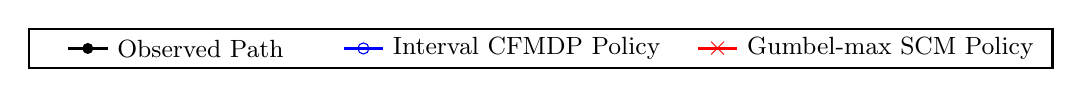
\begin{tikzpicture}[scale=1.0, every node/.style={scale=1.0}]
            \draw[thick, black] (-3, -0.25) rectangle (10, 0.25);
            %
            \draw[black, line width=1pt] (-2.5, 0.0) -- (-2,0.0);
            \fill[black] (-2.25,0.0) circle (2pt); %
            \node[right] at (-2,0.0) {\small Observed Path};
            
            %
            \draw[blue, line width=1pt] (1.0,0.0) -- (1.5,0.0);
            \node[draw=blue, circle, minimum size=4pt, inner sep=0pt] at (1.25,0.0) {}; %
            \node[right] at (1.5,0.0) {\small Interval CFMDP Policy};
            
            %
            \draw[red, line width=1pt] (5.5,0) -- (6,0);
            \node[red] at (5.75,0) {$\boldsymbol{\times}$}; %
            \node[right] at (6,0) {\small Gumbel-max SCM Policy};
        \end{tikzpicture}
    }\\
    %
    \subfigure[\footnotesize Lowest cumulative reward: Interval CFMDP ($312$), Gumbel-max SCM ($312$)]{%
        \resizebox{0.76\columnwidth}{!}{
             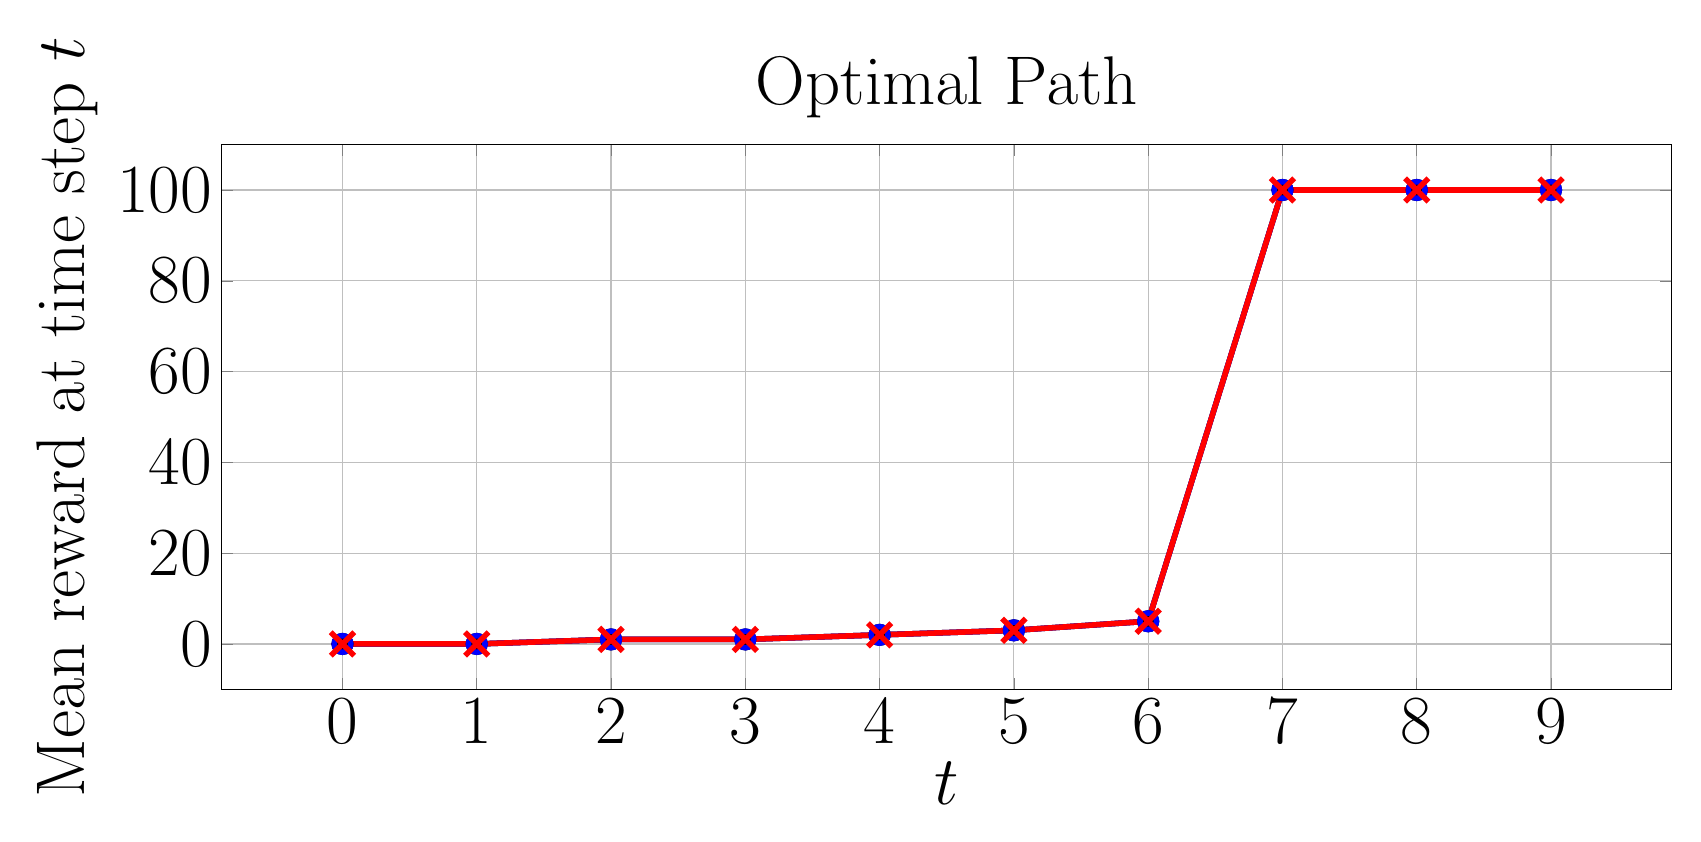
\begin{tikzpicture}
                \begin{axis}[
                    xlabel={$t$},
                    ylabel={Mean reward at time step $t$},
                    title={Optimal Path},
                    grid=both,
                    width=20cm, height=8.5cm,
                    every axis/.style={font=\Huge},
                    %
                ]
                \addplot[
                    color=black, %
                    mark=*, %
                    line width=2pt,
                    mark size=3pt,
                    error bars/.cd,
                    y dir=both, %
                    y explicit, %
                    error bar style={line width=1pt,solid},
                    error mark options={line width=1pt,mark size=4pt,rotate=90}
                ]
                coordinates {
                    (0, 0.0)  +- (0, 0.0)
                    (1, 0.0)  +- (0, 0.0) 
                    (2, 1.0)  +- (0, 0.0) 
                    (3, 1.0)  +- (0, 0.0)
                    (4, 2.0)  +- (0, 0.0)
                    (5, 3.0) +- (0, 0.0)
                    (6, 5.0) +- (0, 0.0)
                    (7, 100.0) +- (0, 0.0)
                    (8, 100.0) +- (0, 0.0)
                    (9, 100.0) +- (0, 0.0)
                };
                %
                \addplot[
                    color=blue, %
                    mark=o, %
                    line width=2pt,
                    mark size=3pt,
                    error bars/.cd,
                    y dir=both, %
                    y explicit, %
                    error bar style={line width=1pt,solid},
                    error mark options={line width=1pt,mark size=4pt,rotate=90}
                ]
                 coordinates {
                    (0, 0.0)  +- (0, 0.0)
                    (1, 0.0)  +- (0, 0.0) 
                    (2, 1.0)  +- (0, 0.0) 
                    (3, 1.0)  +- (0, 0.0)
                    (4, 2.0)  +- (0, 0.0)
                    (5, 3.0) +- (0, 0.0)
                    (6, 5.0) +- (0, 0.0)
                    (7, 100.0) +- (0, 0.0)
                    (8, 100.0) +- (0, 0.0)
                    (9, 100.0) +- (0, 0.0)
                };
                %
                \addplot[
                    color=red, %
                    mark=x, %
                    line width=2pt,
                    mark size=6pt,
                    error bars/.cd,
                    y dir=both, %
                    y explicit, %
                    error bar style={line width=1pt,solid},
                    error mark options={line width=1pt,mark size=4pt,rotate=90}
                ]
                coordinates {
                    (0, 0.0)  +- (0, 0.0)
                    (1, 0.0)  +- (0, 0.0) 
                    (2, 1.0)  +- (0, 0.0) 
                    (3, 1.0)  +- (0, 0.0)
                    (4, 2.0)  +- (0, 0.0)
                    (5, 3.0) +- (0, 0.0)
                    (6, 5.0) +- (0, 0.0)
                    (7, 100.0) +- (0, 0.0)
                    (8, 100.0) +- (0, 0.0)
                    (9, 100.0) +- (0, 0.0)
                };
                \end{axis}
            \end{tikzpicture}
         }
    }
    \hspace{1cm}
    \subfigure[\footnotesize Lowest cumulative reward: Interval CFMDP ($19$), Gumbel-max SCM ($-88$)]{%
         \resizebox{0.76\columnwidth}{!}{
            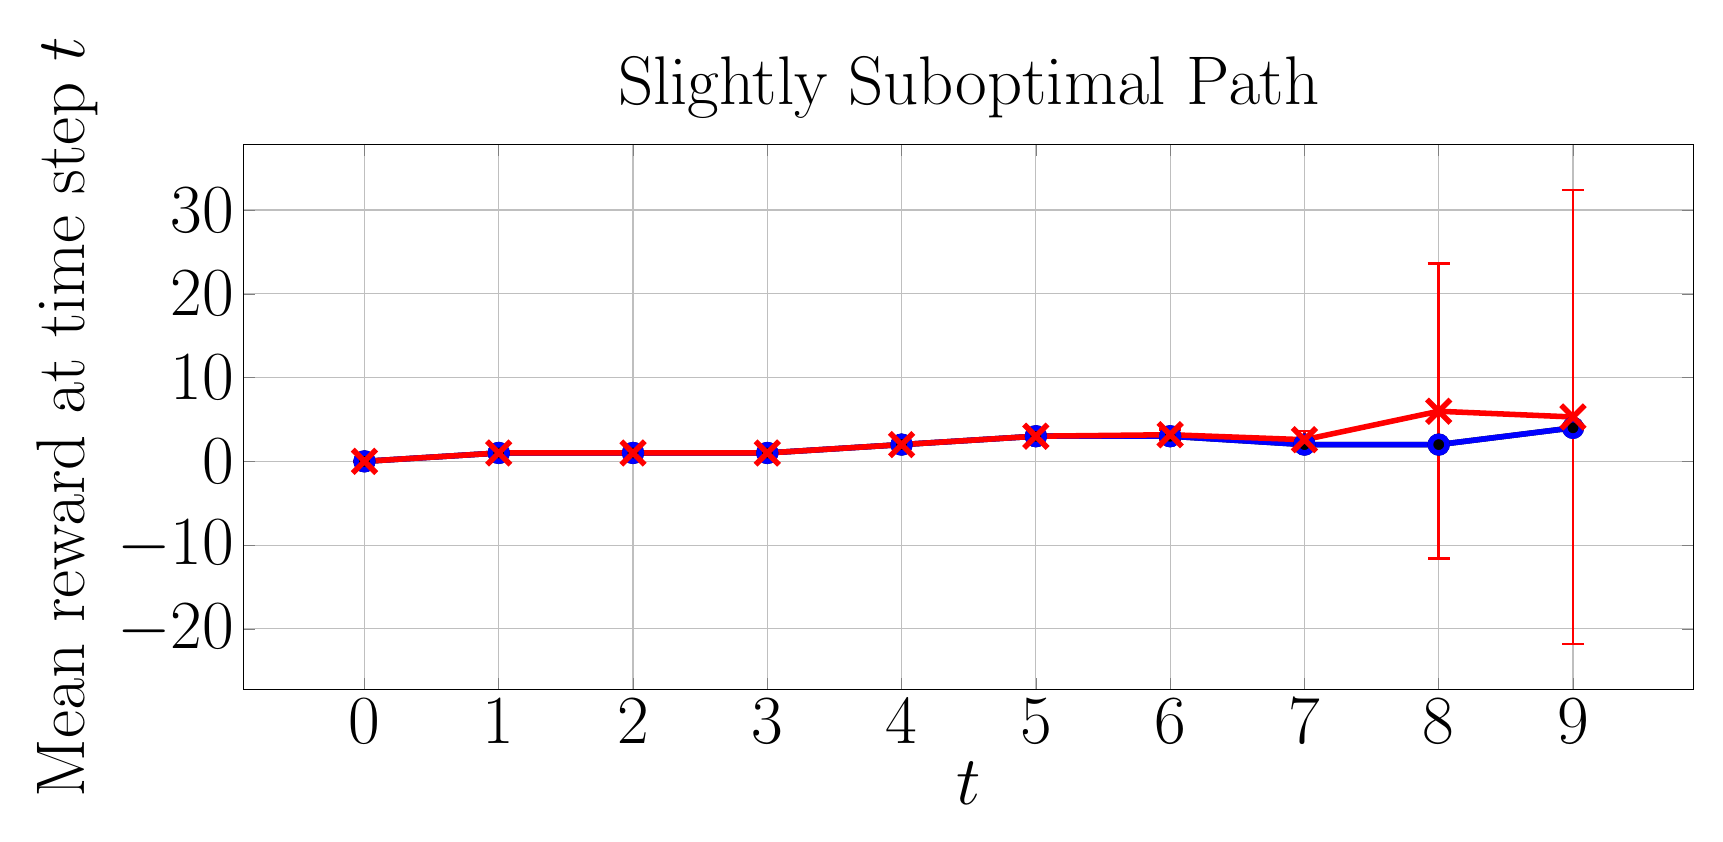
\begin{tikzpicture}
                \begin{axis}[
                    xlabel={$t$},
                    ylabel={Mean reward at time step $t$},
                    title={Slightly Suboptimal Path},
                    grid=both,
                    width=20cm, height=8.5cm,
                    every axis/.style={font=\Huge},
                    %
                ]
                \addplot[
                    color=black, %
                    mark=*, %
                    line width=2pt,
                    mark size=3pt,
                    error bars/.cd,
                    y dir=both, %
                    y explicit, %
                    error bar style={line width=1pt,solid},
                    error mark options={line width=1pt,mark size=4pt,rotate=90}
                ]
              coordinates {
                    (0, 0.0)  +- (0, 0.0)
                    (1, 1.0)  +- (0, 0.0) 
                    (2, 1.0)  +- (0, 0.0) 
                    (3, 1.0)  +- (0, 0.0)
                    (4, 2.0)  +- (0, 0.0)
                    (5, 3.0) +- (0, 0.0)
                    (6, 3.0) +- (0, 0.0)
                    (7, 2.0) +- (0, 0.0)
                    (8, 2.0) +- (0, 0.0)
                    (9, 4.0) +- (0, 0.0)
                };
                %
                \addplot[
                    color=blue, %
                    mark=o, %
                    line width=2pt,
                    mark size=3pt,
                    error bars/.cd,
                    y dir=both, %
                    y explicit, %
                    error bar style={line width=1pt,solid},
                    error mark options={line width=1pt,mark size=4pt,rotate=90}
                ]
              coordinates {
                    (0, 0.0)  +- (0, 0.0)
                    (1, 1.0)  +- (0, 0.0) 
                    (2, 1.0)  +- (0, 0.0) 
                    (3, 1.0)  +- (0, 0.0)
                    (4, 2.0)  +- (0, 0.0)
                    (5, 3.0) +- (0, 0.0)
                    (6, 3.0) +- (0, 0.0)
                    (7, 2.0) +- (0, 0.0)
                    (8, 2.0) +- (0, 0.0)
                    (9, 4.0) +- (0, 0.0)
                };
                %
                \addplot[
                    color=red, %
                    mark=x, %
                    line width=2pt,
                    mark size=6pt,
                    error bars/.cd,
                    y dir=both, %
                    y explicit, %
                    error bar style={line width=1pt,solid},
                    error mark options={line width=1pt,mark size=4pt,rotate=90}
                ]
                coordinates {
                    (0, 0.0)  +- (0, 0.0)
                    (1, 1.0)  +- (0, 0.0) 
                    (2, 1.0)  +- (0, 0.0) 
                    (3, 1.0)  +- (0, 0.0)
                    (4, 2.0)  += (0, 0.0)
                    (5, 3.0)  += (0, 0.0)
                    (6, 3.17847) += (0, 0.62606746) -= (0, 0.62606746)
                    (7, 2.5832885) += (0, 1.04598233) -= (0, 1.04598233)
                    (8, 5.978909) += (0, 17.60137623) -= (0, 17.60137623)
                    (9, 5.297059) += (0, 27.09227512) -= (0, 27.09227512)
                };
                \end{axis}
            \end{tikzpicture}
         }
    }\\[-1.5pt]
    \subfigure[\footnotesize Lowest cumulative reward: Interval CFMDP ($14$), Gumbel-max SCM ($-598$)]{%
         \resizebox{0.76\columnwidth}{!}{
             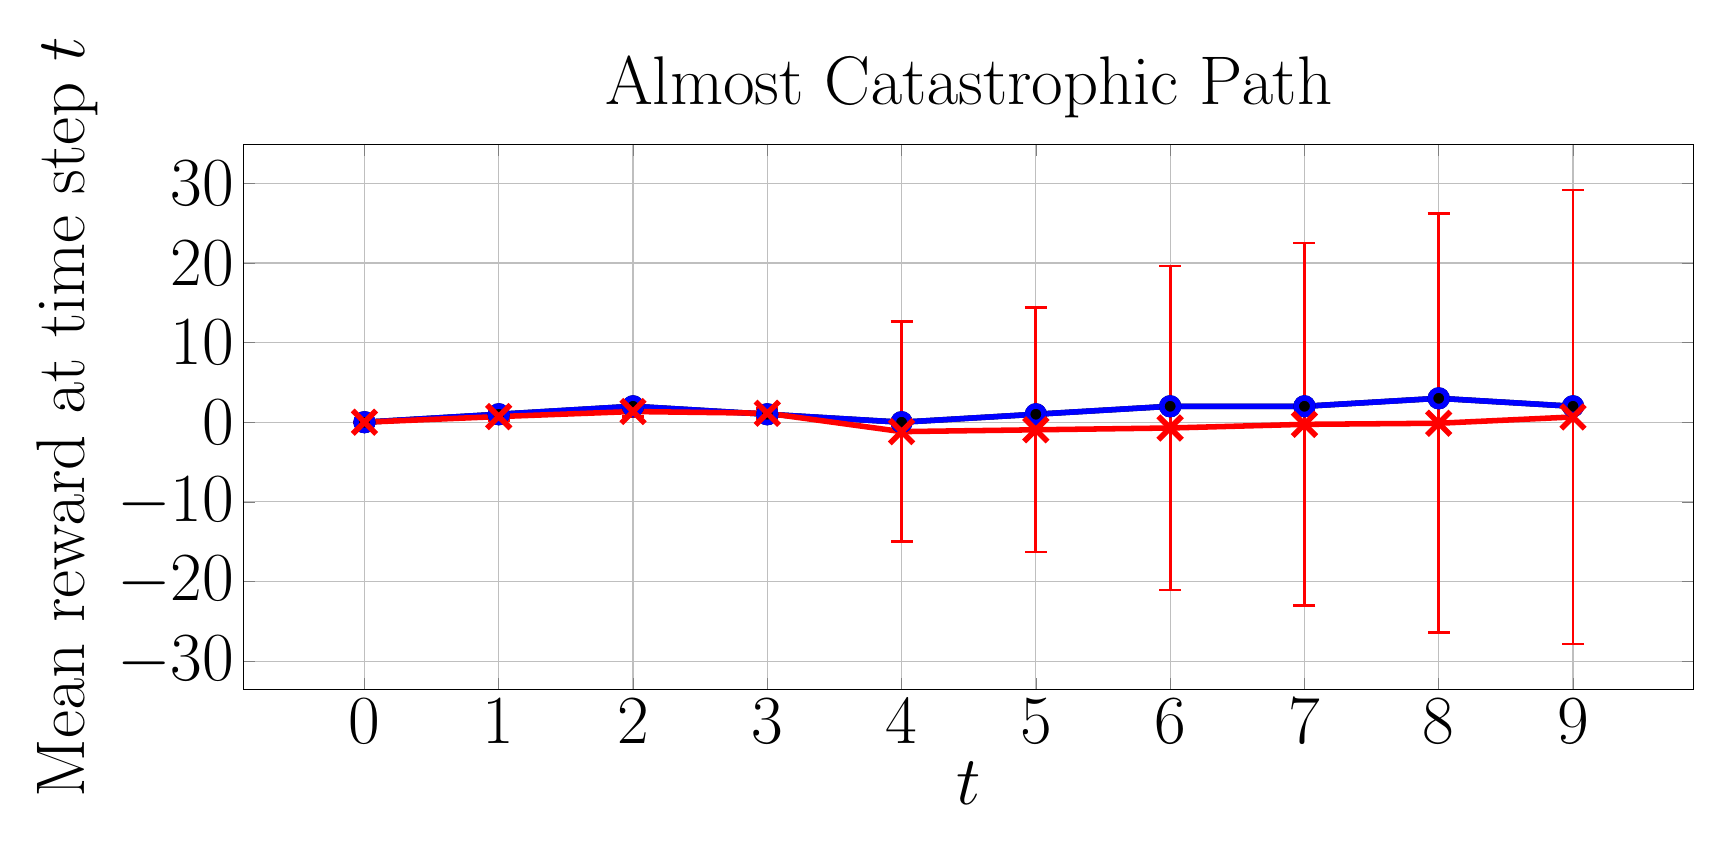
\begin{tikzpicture}
                \begin{axis}[
                    xlabel={$t$},
                    ylabel={Mean reward at time step $t$},
                    title={Almost Catastrophic Path},
                    grid=both,
                    width=20cm, height=8.5cm,
                    every axis/.style={font=\Huge},
                    %
                ]
                \addplot[
                    color=black, %
                    mark=*, %
                    line width=2pt,
                    mark size=3pt,
                    error bars/.cd,
                    y dir=both, %
                    y explicit, %
                    error bar style={line width=1pt,solid},
                    error mark options={line width=1pt,mark size=4pt,rotate=90}
                ]
                coordinates {
                    (0, 0.0)  +- (0, 0.0)
                    (1, 1.0)  +- (0, 0.0) 
                    (2, 2.0)  +- (0, 0.0) 
                    (3, 1.0)  +- (0, 0.0)
                    (4, 0.0)  +- (0, 0.0)
                    (5, 1.0) +- (0, 0.0)
                    (6, 2.0) +- (0, 0.0)
                    (7, 2.0) +- (0, 0.0)
                    (8, 3.0) +- (0, 0.0)
                    (9, 2.0) +- (0, 0.0)
                };
                %
                \addplot[
                    color=blue, %
                    mark=o, %
                    line width=2pt,
                    mark size=3pt,
                    error bars/.cd,
                    y dir=both, %
                    y explicit, %
                    error bar style={line width=1pt,solid},
                    error mark options={line width=1pt,mark size=4pt,rotate=90}
                ]
                coordinates {
                    (0, 0.0)  +- (0, 0.0)
                    (1, 1.0)  +- (0, 0.0) 
                    (2, 2.0)  +- (0, 0.0) 
                    (3, 1.0)  +- (0, 0.0)
                    (4, 0.0)  +- (0, 0.0)
                    (5, 1.0) +- (0, 0.0)
                    (6, 2.0) +- (0, 0.0)
                    (7, 2.0) +- (0, 0.0)
                    (8, 3.0) +- (0, 0.0)
                    (9, 2.0) +- (0, 0.0)
                };
                %
                \addplot[
                    color=red, %
                    mark=x, %
                    line width=2pt,
                    mark size=6pt,
                    error bars/.cd,
                    y dir=both, %
                    y explicit, %
                    error bar style={line width=1pt,solid},
                    error mark options={line width=1pt,mark size=4pt,rotate=90}
                ]
                coordinates {
                    (0, 0.0)  +- (0, 0.0)
                    (1, 0.7065655)  +- (0, 0.4553358) 
                    (2, 1.341673)  +- (0, 0.67091621) 
                    (3, 1.122926)  +- (0, 0.61281824)
                    (4, -1.1821935)  +- (0, 13.82444042)
                    (5, -0.952399)  +- (0, 15.35195457)
                    (6, -0.72672) +- (0, 20.33508414)
                    (7, -0.268983) +- (0, 22.77861454)
                    (8, -0.1310835) +- (0, 26.31013314)
                    (9, 0.65806) +- (0, 28.50670214)
                };
                %
            %
            %
            %
            %
            %
            %
            %
            %
            %
            %
            %
            %
            %
            %
            %
            %
            %
            %
                \end{axis}
            \end{tikzpicture}
         }
    }
    \hspace{1cm}
    \subfigure[\footnotesize Lowest cumulative reward: Interval CFMDP ($-698$), Gumbel-max SCM ($-698$)]{%
         \resizebox{0.76\columnwidth}{!}{
            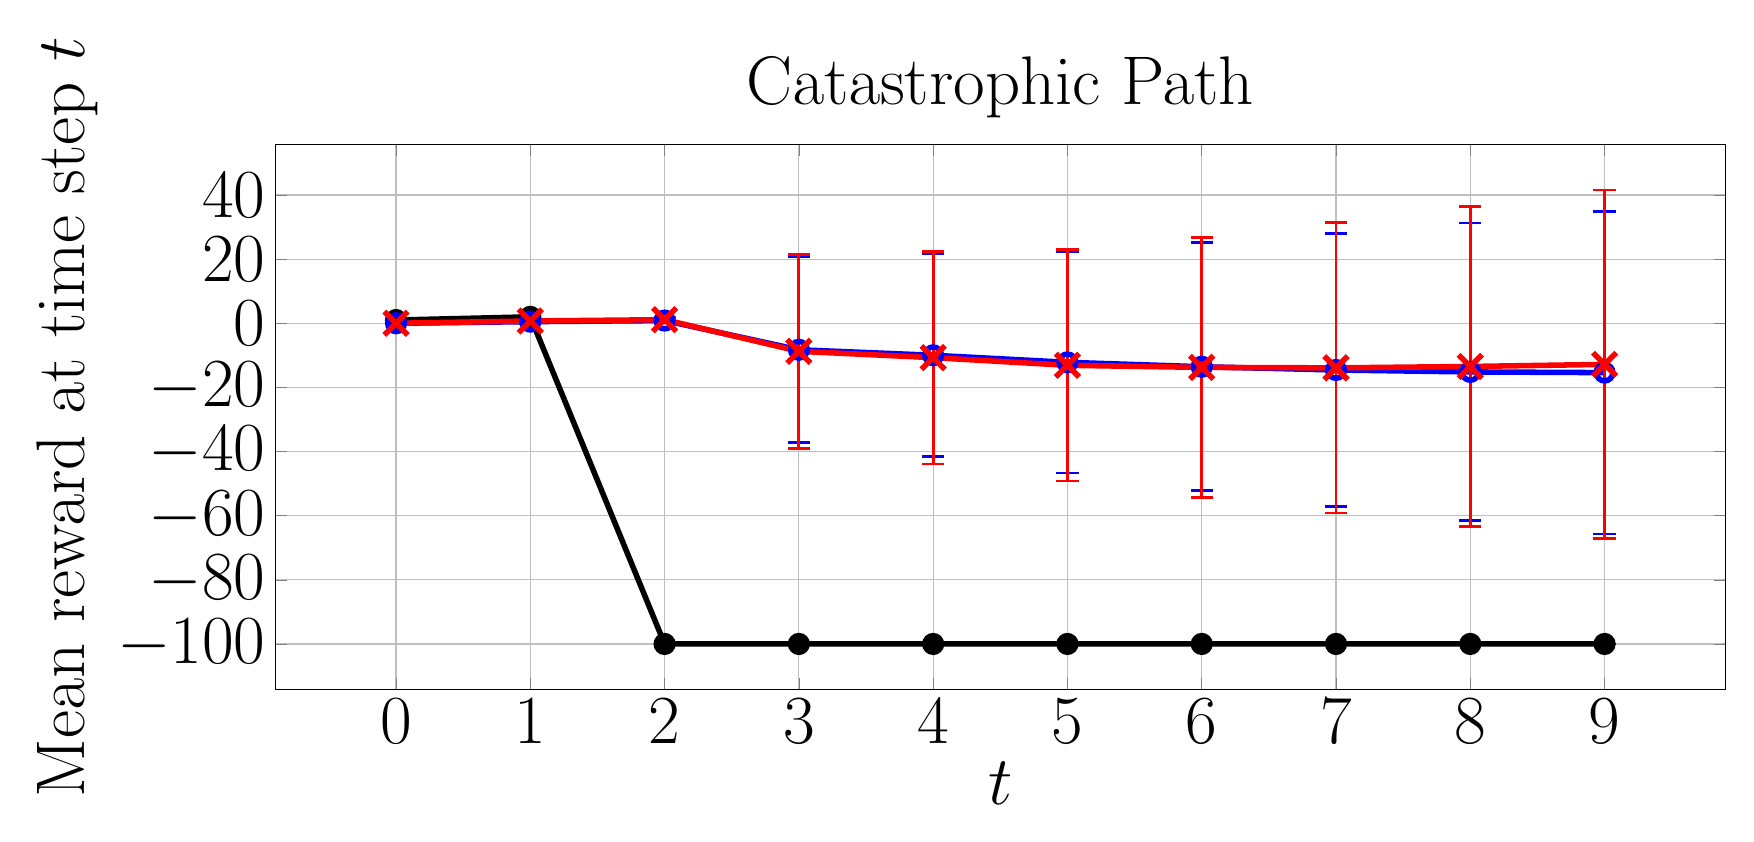
\begin{tikzpicture}
                \begin{axis}[
                    xlabel={$t$},
                    ylabel={Mean reward at time step $t$},
                    title={Catastrophic Path},
                    grid=both,
                    width=20cm, height=8.5cm,
                    every axis/.style={font=\Huge},
                    %
                ]
                \addplot[
                    color=black, %
                    mark=*, %
                    line width=2pt,
                    mark size=3pt,
                    error bars/.cd,
                    y dir=both, %
                    y explicit, %
                    error bar style={line width=1pt,solid},
                    error mark options={line width=1pt,mark size=4pt,rotate=90}
                ]
                coordinates {
                    (0, 1.0)  +- (0, 0.0)
                    (1, 2.0)  +- (0, 0.0) 
                    (2, -100.0)  +- (0, 0.0) 
                    (3, -100.0)  +- (0, 0.0)
                    (4, -100.0)  +- (0, 0.0)
                    (5, -100.0) +- (0, 0.0)
                    (6, -100.0) +- (0, 0.0)
                    (7, -100.0) +- (0, 0.0)
                    (8, -100.0) +- (0, 0.0)
                    (9, -100.0) +- (0, 0.0)
                };
                %
                \addplot[
                    color=blue, %
                    mark=o, %
                    line width=2pt,
                    mark size=3pt,
                    error bars/.cd,
                    y dir=both, %
                    y explicit, %
                    error bar style={line width=1pt,solid},
                    error mark options={line width=1pt,mark size=4pt,rotate=90}
                ]
                coordinates {
                    (0, 0.0)  +- (0, 0.0)
                    (1, 0.504814)  +- (0, 0.49997682) 
                    (2, 0.8439835)  +- (0, 0.76831917) 
                    (3, -8.2709165)  +- (0, 28.93656754)
                    (4, -9.981082)  +- (0, 31.66825363)
                    (5, -12.1776325) +- (0, 34.53463233)
                    (6, -13.556076) +- (0, 38.62845372)
                    (7, -14.574418) +- (0, 42.49603359)
                    (8, -15.1757075) +- (0, 46.41913968)
                    (9, -15.3900395) +- (0, 50.33563368)
                };
                %
                \addplot[
                    color=red, %
                    mark=x, %
                    line width=2pt,
                    mark size=6pt,
                    error bars/.cd,
                    y dir=both, %
                    y explicit, %
                    error bar style={line width=1pt,solid},
                    error mark options={line width=1pt,mark size=4pt,rotate=90}
                ]
                coordinates {
                    (0, 0.0)  +- (0, 0.0)
                    (1, 0.701873)  +- (0, 0.45743556) 
                    (2, 1.1227805)  +- (0, 0.73433129) 
                    (3, -8.7503255)  +- (0, 30.30257976)
                    (4, -10.722092)  +- (0, 33.17618589)
                    (5, -13.10721)  +- (0, 36.0648089)
                    (6, -13.7631645) +- (0, 40.56553451)
                    (7, -13.909043) +- (0, 45.23829402)
                    (8, -13.472517) +- (0, 49.96270296)
                    (9, -12.8278835) +- (0, 54.38618735)
                };
                %
            %
            %
            %
            %
            %
            %
            %
            %
            %
            %
            %
            %
            %
            %
            %
            %
            %
            %
                \end{axis}
            \end{tikzpicture}
         }
    }
    \caption{Average instant reward of CF paths induced by policies on GridWorld $p=0.4$.}
    \label{fig: reward p=0.4}
\end{figure*}

\subsection{Experimental Setup}
To compare policy performance, we measure the average rewards of counterfactual paths induced by our policy and the Gumbel-max policy by uniformly sampling $200$ counterfactual MDPs from the ICFMDP and generating $10,000$ counterfactual paths over each sampled CFMDP. \jl{Since the interval CFMDP depends on the observed path, we select $4$  paths of varying optimality to evaluate how the observed path impacts the performance of both policies: an optimal path, a slightly suboptimal path that could reach the optimal reward with a few changes, a catastrophic path that enters a catastrophic, terminal state with low reward, and an almost catastrophic path that was close to entering a catastrophic state.} When measuring the average probability bound widths and execution time needed to generate the ICFMDPs, we averaged over $20$ randomly generated observed paths
\footnote{Further training details are provided in Appendix \ref{app: training details}, and the code is provided at \href{https://github.com/ddv-lab/robust-cf-inference-in-MDPs}{https://github.com/ddv-lab/robust-cf-inference-in-MDPs}
%
%
.}.

\subsection{GridWorld}
\jl{The GridWorld MDP is a $4 \times 4$ grid where an agent must navigate from the top-left corner to the goal state in the bottom-right corner, avoiding a dangerous terminal state in the centre. At each time step, the agent can move up, down, left, or right, but there is a small probability (controlled by hyper-parameter $p$) of moving in an unintended direction. As the agent nears the goal, the reward for each state increases, culminating in a reward of $+100$ for reaching the goal. Entering the dangerous state results in a penalty of $-100$. We use two versions of GridWorld: a less stochastic version with $p=0.9$ (i.e., $90$\% chance of moving in the chosen direction) and a more stochastic version with $p=0.4$.}

\paragraph{GridWorld ($p=0.9$)}
When $p=0.9$, the counterfactual probability bounds are typically narrow (see Table \ref{tab:nonzero_probs} for average measurements). Consequently, as shown in Figure \ref{fig: reward p=0.9}, both policies are nearly identical and perform similarly well across the optimal, slightly suboptimal, and catastrophic paths.
%
However, for the almost catastrophic path, the interval CFMDP path is more conservative and follows the observed path more closely (as this is where the probability bounds are narrowest), which typically requires one additional step to reach the goal state than the Gumbel-max SCM policy.
%

\paragraph{GridWorld ($p=0.4$)}
\jl{When $p=0.4$, the GridWorld environment becomes more uncertain, increasing the risk of entering the dangerous state even if correct actions are chosen. Thus, as shown in Figure \ref{fig: reward p=0.4}, the interval CFMDP policy adopts a more conservative approach, avoiding deviation from the observed policy if it cannot guarantee higher counterfactual rewards (see the slightly suboptimal and almost catastrophic paths), whereas the Gumbel-max SCM is inconsistent: it can yield higher rewards, but also much lower rewards, reflected in the wide error bars.} For the catastrophic path, both policies must deviate from the observed path to achieve a higher reward and, in this case, perform similarly.
%
%
%
%
\subsection{Sepsis}
The Sepsis MDP \citep{oberst2019counterfactual} simulates trajectories of Sepsis patients. Each state consists of four vital signs (heart rate, blood pressure, oxygen concentration, and glucose levels), categorised as low, normal, or high.
and three treatments that can be toggled on/off at each time step (8 actions in total). Unlike \citet{oberst2019counterfactual}, we scale rewards based on the number of out-of-range vital signs, between $-1000$ (patient dies) and $1000$ (patient discharged). \jl{Like the GridWorld $p=0.4$ experiment, the Sepsis MDP is highly uncertain, as many states are equally likely to lead to optimal and poor outcomes. Thus, as shown in Figure \ref{fig: reward sepsis}, both policies follow the observed optimal and almost catastrophic paths to guarantee rewards are no worse than the observation.} However, improving the catastrophic path requires deviating from the observation. Here, the Gumbel-max SCM policy, on average, performs better than the interval CFMDP policy. But, since both policies have lower bounds clipped at $-1000$, neither policy reliably improves over the observation. In contrast, for the slightly suboptimal path, the interval CFMDP policy performs significantly better, shown by its higher lower bounds. 
Moreover, in these two cases, the worst-case counterfactual path generated by the interval CFMDP policy is better than that of the Gumbel-max SCM policy,
indicating its greater robustness.
%
\begin{figure*}
    \centering
     \resizebox{0.6\textwidth}{!}{
        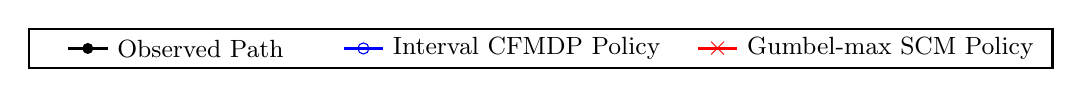
\begin{tikzpicture}[scale=1.0, every node/.style={scale=1.0}]
            \draw[thick, black] (-3, -0.25) rectangle (10, 0.25);
            %
            \draw[black, line width=1pt] (-2.5, 0.0) -- (-2,0.0);
            \fill[black] (-2.25,0.0) circle (2pt); %
            \node[right] at (-2,0.0) {\small Observed Path};
            
            %
            \draw[blue, line width=1pt] (1.0,0.0) -- (1.5,0.0);
            \node[draw=blue, circle, minimum size=4pt, inner sep=0pt] at (1.25,0.0) {}; %
            \node[right] at (1.5,0.0) {\small Interval CFMDP Policy};
            
            %
            \draw[red, line width=1pt] (5.5,0) -- (6,0);
            \node[red] at (5.75,0) {$\boldsymbol{\times}$}; %
            \node[right] at (6,0) {\small Gumbel-max SCM Policy};
        \end{tikzpicture}
    }\\
    \subfigure[\footnotesize Lowest cumulative reward: Interval CFMDP ($8000$), Gumbel-max SCM ($8000$)]{%
         \resizebox{0.76\columnwidth}{!}{
             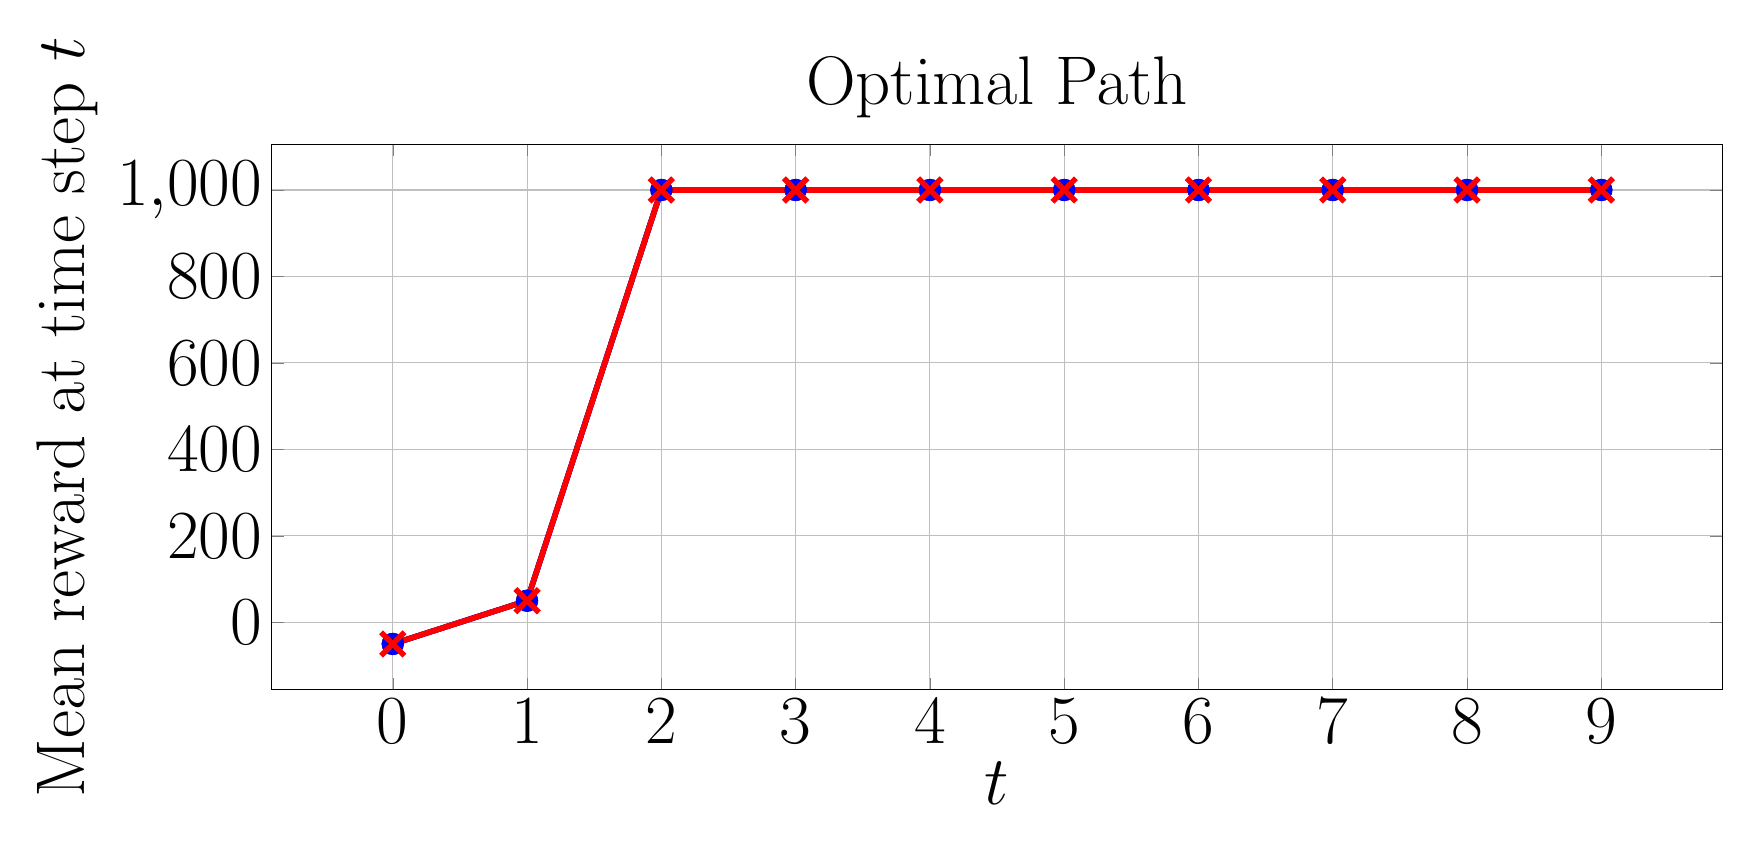
\begin{tikzpicture}
                \begin{axis}[
                    xlabel={$t$},
                    ylabel={Mean reward at time step $t$},
                    title={Optimal Path},
                    grid=both,
                    width=20cm, height=8.5cm,
                    every axis/.style={font=\Huge},
                    %
                ]
                \addplot[
                    color=black, %
                    mark=*, %
                    line width=2pt,
                    mark size=3pt,
                ]
                coordinates {
                    (0, -50.0)
                    (1, 50.0)
                    (2, 1000.0)
                    (3, 1000.0)
                    (4, 1000.0)
                    (5, 1000.0)
                    (6, 1000.0)
                    (7, 1000.0)
                    (8, 1000.0)
                    (9, 1000.0)
                };
                %
                \addplot[
                    color=blue, %
                    mark=o, %
                    line width=2pt,
                    mark size=3pt,
                    error bars/.cd,
                    y dir=both, %
                    y explicit, %
                    error bar style={line width=1pt,solid},
                    error mark options={line width=1pt,mark size=4pt,rotate=90}
                ]
                coordinates {
                    (0, -50.0)  +- (0, 0.0)
                    (1, 50.0)  +- (0, 0.0) 
                    (2, 1000.0)  +- (0, 0.0) 
                    (3, 1000.0)  +- (0, 0.0)
                    (4, 1000.0)  +- (0, 0.0)
                    (5, 1000.0) +- (0, 0.0)
                    (6, 1000.0) +- (0, 0.0)
                    (7, 1000.0) +- (0, 0.0)
                    (8, 1000.0) +- (0, 0.0)
                    (9, 1000.0) +- (0, 0.0)
                };
                %
                \addplot[
                    color=red, %
                    mark=x, %
                    line width=2pt,
                    mark size=6pt,
                    error bars/.cd,
                    y dir=both, %
                    y explicit, %
                    error bar style={line width=1pt,solid},
                    error mark options={line width=1pt,mark size=4pt,rotate=90}
                ]
                coordinates {
                    (0, -50.0)  +- (0, 0.0)
                    (1, 50.0)  +- (0, 0.0) 
                    (2, 1000.0)  +- (0, 0.0) 
                    (3, 1000.0)  +- (0, 0.0)
                    (4, 1000.0)  +- (0, 0.0)
                    (5, 1000.0) +- (0, 0.0)
                    (6, 1000.0) +- (0, 0.0)
                    (7, 1000.0) +- (0, 0.0)
                    (8, 1000.0) +- (0, 0.0)
                    (9, 1000.0) +- (0, 0.0)
                };
                %
                \end{axis}
            \end{tikzpicture}
         }
    }
    \hspace{1cm}
    \subfigure[\footnotesize Lowest cumulative reward: Interval CFMDP ($-5980$), Gumbel-max SCM ($-8000$)]{%
         \resizebox{0.76\columnwidth}{!}{
            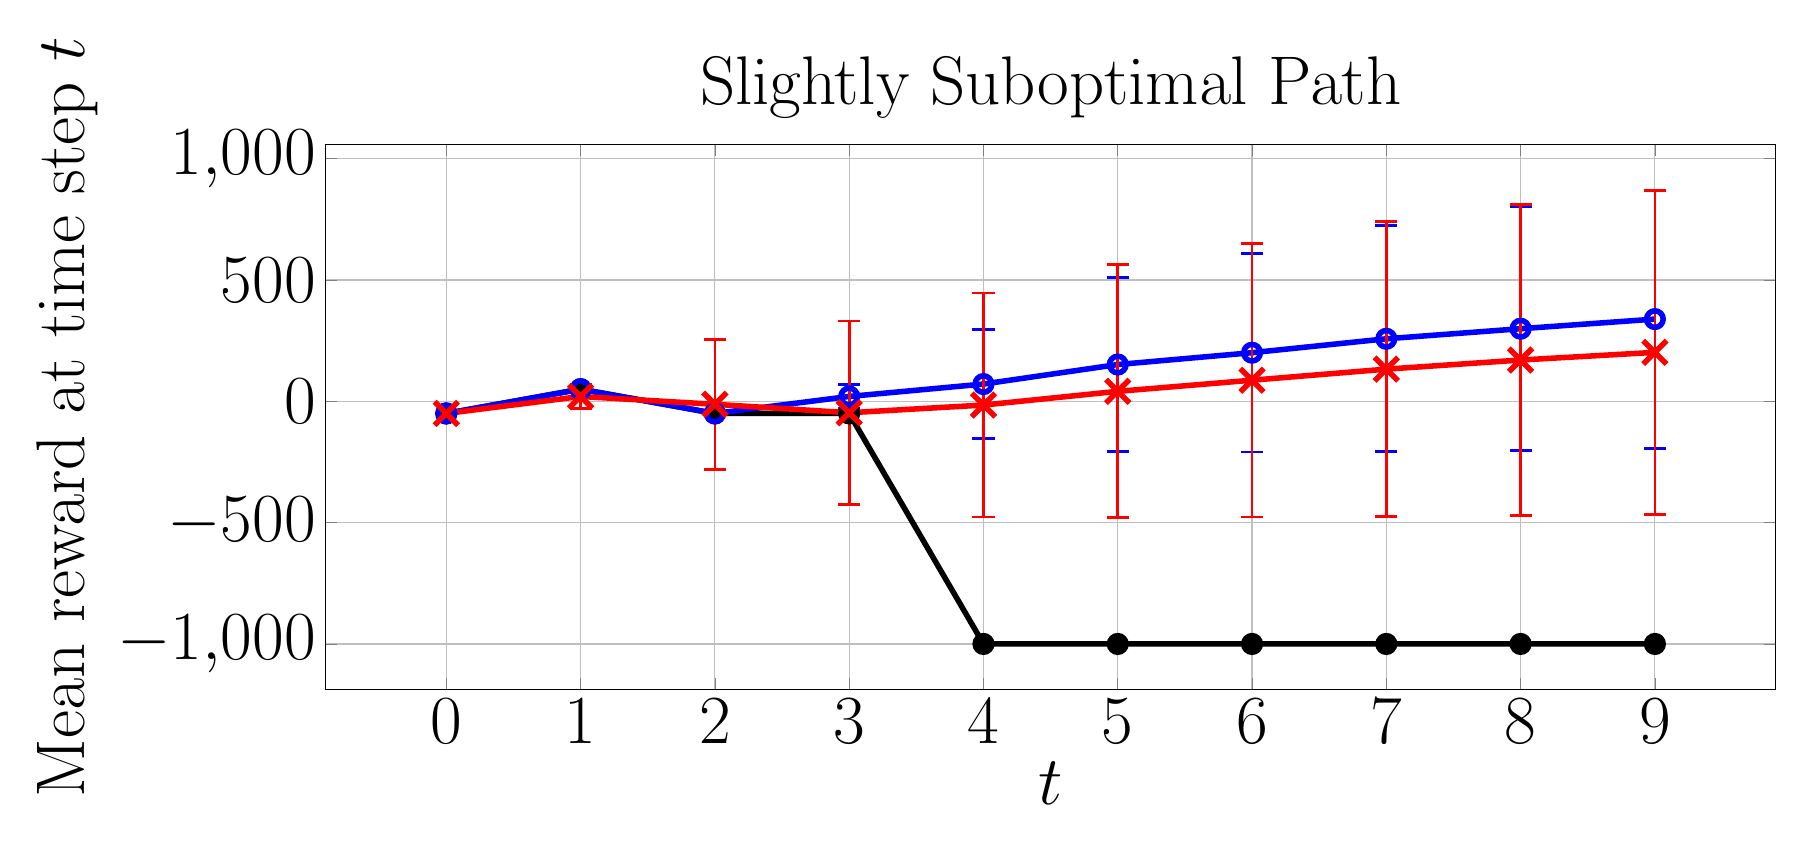
\begin{tikzpicture}
                \begin{axis}[
                    xlabel={$t$},
                    ylabel={Mean reward at time step $t$},
                    title={Slightly Suboptimal Path},
                    grid=both,
                    width=20cm, height=8.5cm,
                    every axis/.style={font=\Huge},
                    %
                ]
               \addplot[
                    color=black, %
                    mark=*, %
                    line width=2pt,
                    mark size=3pt,
                ]
                coordinates {
                    (0, -50.0)
                    (1, 50.0)
                    (2, -50.0)
                    (3, -50.0)
                    (4, -1000.0)
                    (5, -1000.0)
                    (6, -1000.0)
                    (7, -1000.0)
                    (8, -1000.0)
                    (9, -1000.0)
                };
                %
                \addplot[
                    color=blue, %
                    mark=o, %
                    line width=2pt,
                    mark size=3pt,
                    error bars/.cd,
                    y dir=both, %
                    y explicit, %
                    error bar style={line width=1pt,solid},
                    error mark options={line width=1pt,mark size=4pt,rotate=90}
                ]
                coordinates {
                    (0, -50.0)  +- (0, 0.0)
                    (1, 50.0)  +- (0, 0.0) 
                    (2, -50.0)  +- (0, 0.0) 
                    (3, 20.0631)  +- (0, 49.97539413)
                    (4, 71.206585)  +- (0, 226.02033693)
                    (5, 151.60797) +- (0, 359.23292559)
                    (6, 200.40593) +- (0, 408.86185176)
                    (7, 257.77948) +- (0, 466.10372804)
                    (8, 299.237465) +- (0, 501.82579506)
                    (9, 338.9129) +- (0, 532.06124996)
                };
                %
                \addplot[
                    color=red, %
                    mark=x, %
                    line width=2pt,
                    mark size=6pt,
                    error bars/.cd,
                    y dir=both, %
                    y explicit, %
                    error bar style={line width=1pt,solid},
                    error mark options={line width=1pt,mark size=4pt,rotate=90}
                ]
                coordinates {
                    (0, -50.0)  +- (0, 0.0)
                    (1, 20.00736)  +- (0, 49.99786741) 
                    (2, -12.282865)  +- (0, 267.598755) 
                    (3, -47.125995)  +- (0, 378.41755832)
                    (4, -15.381965)  +- (0, 461.77616558)
                    (5, 41.15459) +- (0, 521.53189262)
                    (6, 87.01595) +- (0, 564.22243126 )
                    (7, 132.62376) +- (0, 607.31338037)
                    (8, 170.168145) +- (0, 641.48013693)
                    (9, 201.813135) +- (0, 667.29441777)
                };
                %
                %
                %
                %
                %
                %
                %
                %
                %
                %
                %
                %
                %
                %
                %
                %
                %
                %
                %
                \end{axis}
            \end{tikzpicture}
         }
    }\\[-1.5pt]
    \subfigure[\footnotesize Lowest cumulative reward: Interval CFMDP ($100$), Gumbel-max SCM ($100$)]{%
         \resizebox{0.76\columnwidth}{!}{
             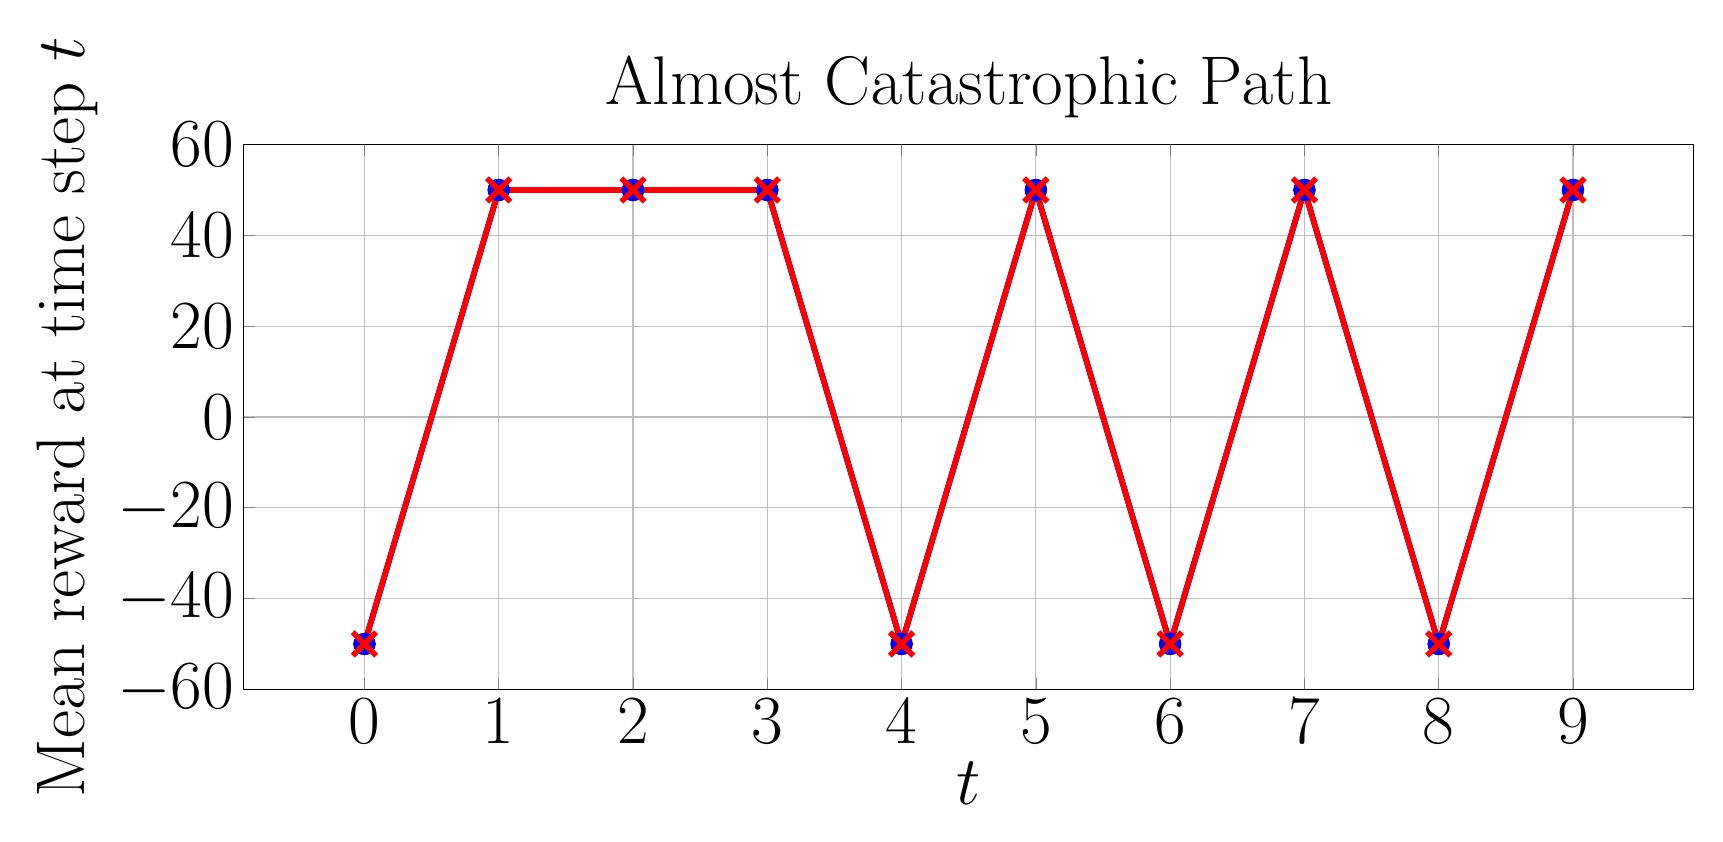
\begin{tikzpicture}
                \begin{axis}[
                    xlabel={$t$},
                    ylabel={Mean reward at time step $t$},
                    title={Almost Catastrophic Path},
                    grid=both,
                    every axis/.style={font=\Huge},
                    width=20cm, height=8.5cm,
                    %
                ]
               \addplot[
                    color=black, %
                    mark=*, %
                    line width=2pt,
                    mark size=3pt,
                ]
                coordinates {
                    (0, -50.0)
                    (1, 50.0)
                    (2, 50.0)
                    (3, 50.0)
                    (4, -50.0)
                    (5, 50.0)
                    (6, -50.0)
                    (7, 50.0)
                    (8, -50.0)
                    (9, 50.0)
                };
                %
                %
                \addplot[
                    color=blue, %
                    mark=o, %
                    line width=2pt,
                    mark size=3pt,
                    error bars/.cd,
                    y dir=both, %
                    y explicit, %
                    error bar style={line width=1pt,solid},
                    error mark options={line width=1pt,mark size=4pt,rotate=90}
                ]
                coordinates {
                    (0, -50.0)  +- (0, 0.0)
                    (1, 50.0)  +- (0, 0.0) 
                    (2, 50.0)  +- (0, 0.0) 
                    (3, 50.0)  +- (0, 0.0)
                    (4, -50.0)  +- (0, 0.0)
                    (5, 50.0) +- (0, 0.0)
                    (6, -50.0) +- (0, 0.0)
                    (7, 50.0) +- (0, 0.0)
                    (8, -50.0) +- (0, 0.0)
                    (9, 50.0) +- (0, 0.0)
                };
                %
                \addplot[
                    color=red, %
                    mark=x, %
                    line width=2pt,
                    mark size=6pt,
                    error bars/.cd,
                    y dir=both, %
                    y explicit, %
                    error bar style={line width=1pt,solid},
                    error mark options={line width=1pt,mark size=4pt,rotate=90}
                ]
                coordinates {
                    (0, -50.0)  +- (0, 0.0)
                    (1, 50.0)  +- (0, 0.0) 
                    (2, 50.0)  +- (0, 0.0) 
                    (3, 50.0)  +- (0, 0.0)
                    (4, -50.0)  +- (0, 0.0)
                    (5, 50.0) +- (0, 0.0)
                    (6, -50.0) +- (0, 0.0)
                    (7, 50.0) +- (0, 0.0)
                    (8, -50.0) +- (0, 0.0)
                    (9, 50.0) +- (0, 0.0)
                };
                %
                %
                %
                %
                %
                %
                %
                %
                %
                %
                %
                %
                %
                %
                %
                %
                %
                %
                %
                \end{axis}
            \end{tikzpicture}
         }
    }
    \hspace{1cm}
    \subfigure[\footnotesize Lowest cumulative reward: Interval CFMDP ($-7150$), Gumbel-max SCM ($-9050$)]{%
         \resizebox{0.76\columnwidth}{!}{
            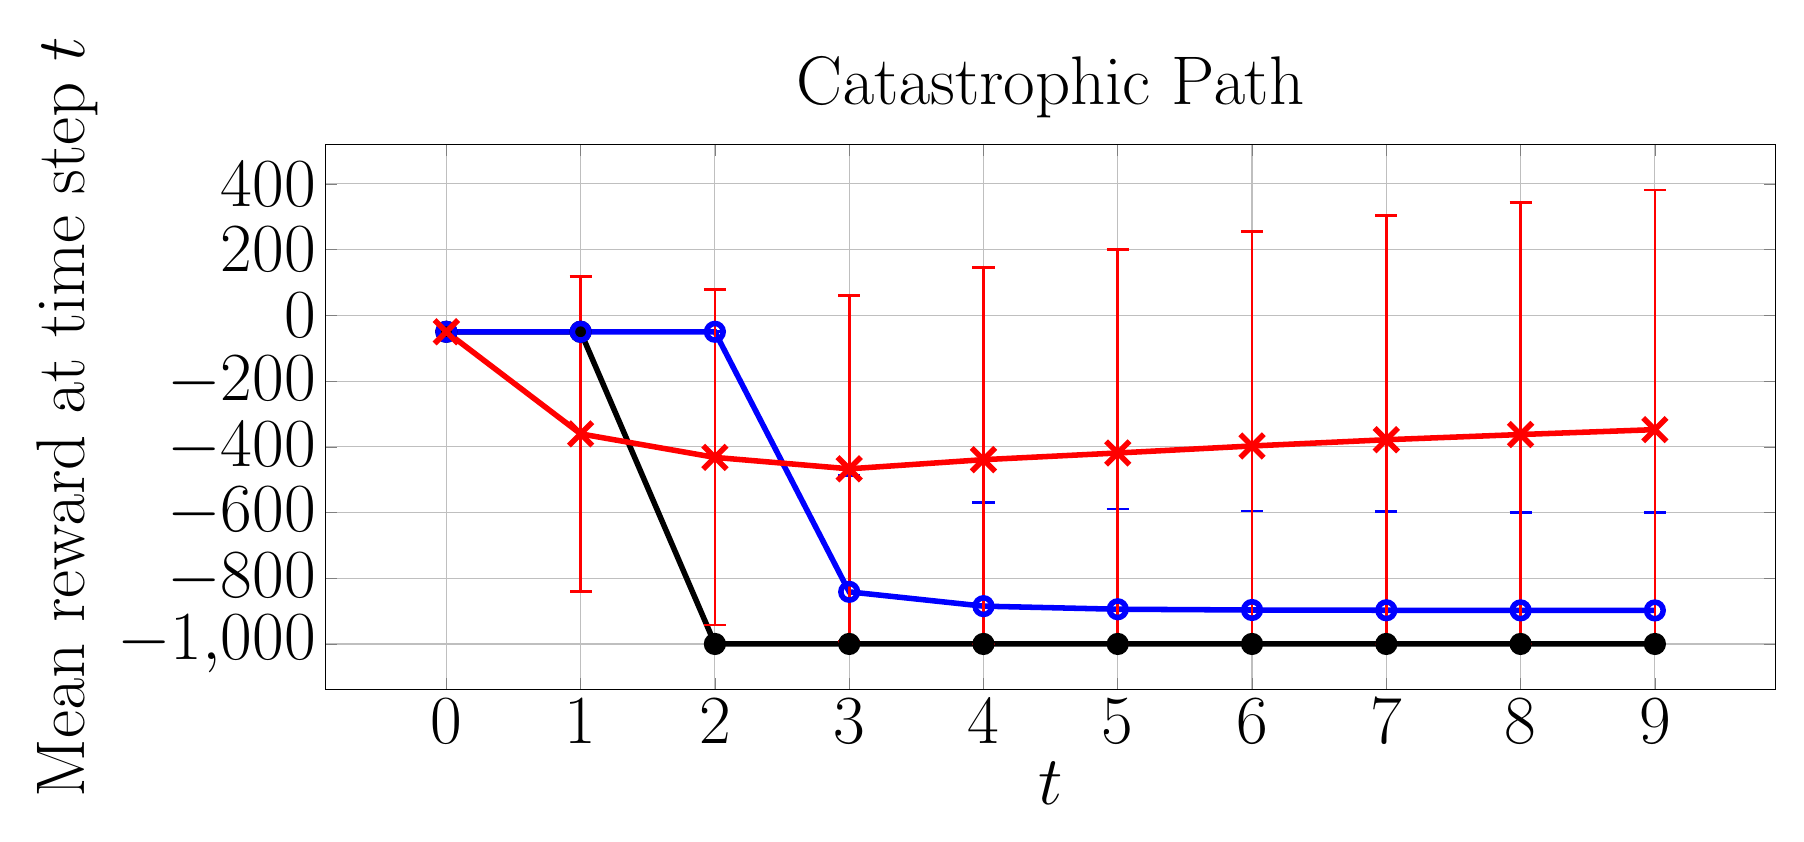
\begin{tikzpicture}
                \begin{axis}[
                    xlabel={$t$},
                    ylabel={Mean reward at time step $t$},
                    title={Catastrophic Path},
                    grid=both,
                    width=20cm, height=8.5cm,
                    every axis/.style={font=\Huge},
                    %
                ]
               \addplot[
                    color=black, %
                    mark=*, %
                    line width=2pt,
                    mark size=3pt,
                ]
                coordinates {
                    (0, -50.0)
                    (1, -50.0)
                    (2, -1000.0)
                    (3, -1000.0)
                    (4, -1000.0)
                    (5, -1000.0)
                    (6, -1000.0)
                    (7, -1000.0)
                    (8, -1000.0)
                    (9, -1000.0)
                };
                %
                %
                \addplot[
                    color=blue, %
                    mark=o, %
                    line width=2pt,
                    mark size=3pt,
                    error bars/.cd,
                    y dir=both, %
                    y explicit, %
                    error bar style={line width=1pt,solid},
                    error mark options={line width=1pt,mark size=4pt,rotate=90}
                ]
                coordinates {
                    (0, -50.0)  +- (0, 0.0)
                    (1, -50.0)  +- (0, 0.0) 
                    (2, -50.0)  +- (0, 0.0) 
                    (3, -841.440725)  += (0, 354.24605512) -= (0, 158.559275)
                    (4, -884.98225)  += (0, 315.37519669) -= (0, 115.01775)
                    (5, -894.330425) += (0, 304.88572805) -= (0, 105.669575)
                    (6, -896.696175) += (0, 301.19954514) -= (0, 103.303825)
                    (7, -897.4635) += (0, 299.61791279) -= (0, 102.5365)
                    (8, -897.77595) += (0, 298.80392585) -= (0, 102.22405)
                    (9, -897.942975) += (0, 298.32920557) -= (0, 102.057025)
                };
                %
                \addplot[
                    color=red, %
                    mark=x, %
                    line width=2pt,
                    mark size=6pt,
                    error bars/.cd,
                    y dir=both, %
                    y explicit, %
                    error bar style={line width=1pt,solid},
                    error mark options={line width=1pt,mark size=4pt,rotate=90}
                ]
            coordinates {
                    (0, -50.0)  +- (0, 0.0)
                    (1, -360.675265)  +- (0, 479.39812699) 
                    (2, -432.27629)  +- (0, 510.38620897) 
                    (3, -467.029545)  += (0, 526.36009628) -= (0, 526.36009628)
                    (4, -439.17429)  += (0, 583.96638919) -= (0, 560.82571)
                    (5, -418.82704) += (0, 618.43027478) -= (0, 581.17296)
                    (6, -397.464895) += (0, 652.67322574) -= (0, 602.535105)
                    (7, -378.49052) += (0, 682.85407033) -= (0, 621.50948)
                    (8, -362.654195) += (0, 707.01412023) -= (0, 637.345805)
                    (9, -347.737935) += (0, 729.29076479) -= (0, 652.262065)
                };
                %
                %
                %
                %
                %
                %
                %
                %
                %
                %
                %
                %
                %
                %
                %
                %
                %
                %
                %
                \end{axis}
            \end{tikzpicture}
         }
    }
    \caption{Average instant reward of CF paths induced by policies on Sepsis.}
    \label{fig: reward sepsis}
\end{figure*}

%
%
%
\subsection{Interval CFMDP Bounds}
%
%
Table \ref{tab:nonzero_probs} presents the mean counterfactual probability bound widths (excluding transitions where the upper bound is $0$) for each MDP, averaged over 20 observed paths. We compare the bounds under counterfactual stability (CS) and monotonicity (M) assumptions, CS alone, and no assumptions. This shows that the assumptions marginally reduce the bound widths, indicating the assumptions tighten the bounds without excluding too many causal models, as intended.
\renewcommand{\arraystretch}{1}

\begin{table}
\centering
\caption{Mean width of counterfactual probability bounds}
\resizebox{0.8\columnwidth}{!}{%
\begin{tabular}{|c|c|c|c|}
\hline
\multirow{2}{*}{\textbf{Environment}} & \multicolumn{3}{c|}{\textbf{Assumptions}} \\ \cline{2-4}
 & \textbf{CS + M} & \textbf{CS} & \textbf{None\tablefootnote{\jl{Equivalent to \citet{li2024probabilities}'s bounds (see Section \ref{sec: equivalence with Li}).}}} \\ \hline
\textbf{GridWorld} ($p=0.9$) & 0.0817 & 0.0977 & 0.100 \\ \hline
\textbf{GridWorld} ($p=0.4$) & 0.552  & 0.638  & 0.646 \\ \hline
\textbf{Sepsis} & 0.138 & 0.140 & 0.140 \\ \hline
\end{tabular}
}
\label{tab:nonzero_probs}
\end{table}


\subsection{Execution Times}
Table \ref{tab: times} compares the average time needed to generate the interval CFMDP vs.\ the Gumbel-max SCM CFMDP for 20 observations.
The GridWorld algorithms were run single-threaded, while the Sepsis experiments were run in parallel.
Generating the interval CFMDP is significantly faster as it uses exact analytical bounds, whereas the Gumbel-max CFMDP requires sampling from the Gumbel distribution to estimate counterfactual transition probabilities. \jl{Since constructing the counterfactual MDP models is the main bottleneck in both approaches, ours is more efficient overall and suitable for larger MDPs.}
\begin{table}
\centering
\caption{Mean execution time to generate CFMDPs}
\resizebox{0.99\columnwidth}{!}{%
\begin{tabular}{|c|c|c|}
\hline
\multirow{2}{*}{\textbf{Environment}} & \multicolumn{2}{c|}{\textbf{Mean Execution Time (s)}} \\ \cline{2-3} 
                                      & \textbf{Interval CFMDP} & \textbf{Gumbel-max CFMDP} \\ \hline
\textbf{GridWorld ($p=0.9$) }                  & 0.261                   & 56.1                      \\ \hline
\textbf{GridWorld ($p=0.4$)  }                 & 0.336                   & 54.5                      \\ \hline
\textbf{Sepsis}                                 & 688                     & 2940                      \\ \hline
\end{tabular}%
}
\label{tab: times}
\end{table}


%We discuss the results of the effectiveness of applying program transformations on the out-of-scope data. Table ~\ref{Tab:evaluation} represents the statistics of our experimental results. In addition to Table~\ref{Tab:evaluation}, we also show the statistics of number of inputs that program transformation has been applied, the number of correctly predicted and incorrectly predicted inputs of the total inputs by comparing those to the ground truth data, and number of transformed inputs that convert a correct prediction to incorrect vice versa in Table~\ref{Tab:stts}.


\textit{Baseline}: CodeImprove is the first technique to improve the code model's performance through program transformations. Thus, we cannot find direct baselines for comparison. To address this, we draw inspiration from a technique in the image domain for comparative analysis, i.e. the InputReflector \textcolor{blue}{\textbf{(IRef)}}~\cite{xiao2022repairing} that detects deviating inputs and substitutes them with the most similar sample from the training set. We are unable to include CodeDenoise~\cite{tian2023code} as a baseline due to the evaluation methods of this work, which splits the test set into two subsets as T1 and T2 and subsequently assesses results on T2 set. However, the splitting criteria of datasets is not provided in the project website. Moreover, the work is similar to the adversarial style, which denoises the program identifiers and corrects the program with the supervision of the model's predictions. CodeImprove demonstrates better performance compared to CodeDenoise~\cite{tian2023code} where it only fixes 20.45\% of inputs while CodeImprove fixes 32.8\% for defect prediction task on the CodeBERT model.

%We borrowed the ideas from two techniques in the image domain for comparison. Input reflector (IR)~\cite{xiao2022repairing} and interpretable technique (IT)~\cite{mohasel2023interpretable} identifies deviating inputs and replace with the samples in training set. %We ignore the work in ~\cite{tian2023fly} because the work identifies noisy identifiers in the dataset by applying perturbations and then clease these identifiers. Although, such technique can help in improving model performance, it requires to generate multiple samples for input validation by applying perturbations for multiple identifiers. Moreover, the work splits the test set into two sets, thus making the sample size even smaller. 

\textit{Process}: \textcolor{blue}{\textbf{IRef}} employs two models, namely the siamese network~\cite{he2018twofold} and the quadruple network~\cite{xiao2022repairing}, to detect deviating inputs and repair them, respectively. During training, these models rely on three datasets: the original set, the transformed (human recognizable) set, and the extremely transformed (human unrecognizable) set. These two transformed sets are generated by applying different degrees of transformation to the original training set. However, generating such datasets for code data poses challenges as code inputs cannot rely on a degree of transformation like in image data. Therefore, we utilized only two sets: the original set and its transformed version. We configured the loss functions employed in the \textcolor{blue}{IRef} accordingly for these two sets. We leverage the hidden layer outputs from the original model and feed them to the siamese network and quadruple network. Subsequently, we search for similar data in the training set to repair the out-of-scope inputs by exchanging the labels of the most similar training sample. For CodeImprove, we employed all 15 transformations during the crossover step. The effectiveness is measured using various metrics, including accuracy, precision, recall, F1-score, relative improvement (RI), correction success rate (CSR), and mis-correction rate (MCR).   
%%edited Table~\ref{Tab:performance} presents a detailed comparison between CodeImprove and \textcolor{blue}{IRef}, illustrating that CodeImprove consistently outperforms \textcolor{blue}{IRef} across various metrics. 

\textit{Result: }Table~\ref{Tab:performance} \textcolor{blue}{presents} the comparison \textcolor{blue}{between CodeImprove and \textcolor{blue}{IRef}, illustrating that CodeImprove consistently outperforms \textcolor{blue}{IRef}.}
%results comparing CodeImprove with IR. From this table, we found that CodeImprove always performs better than IR.
\textcolor{blue}{Notably}, we observe the following: (1) CodeImprove consistently achieved the best model improvements ranging upto 8.78\% in accuracy, 8.48\% in precision, 16.9\% in recall, and 13.5\% in F1-score on all the subjects; (2) CodeImprove is capable of correcting around 23.1\% to 39.9\% of the mispredicted inputs on both vulnerability detection and defect prediction tasks; (3) The RI measurement shows significant improvement for RoBERTa models on both the tasks. On other models, CodeImprove shows \textcolor{blue}{a RI ranging from} 21.1\% to 51.28\%; (4) Techniques employed in the image domain \textcolor{blue}{\textbf{(IRef)}} cannot be applied to code data\textcolor{blue}{. Our results indicate that \textcolor{blue}{IRef} negatively impacts the}, 
%as our results show that IR hurts
 model performance for the CodeBERT model on both vulnerability detection and defect prediction tasks. Moreover, the defect prediction task shows performance discrepancy on all models for \textcolor{blue}{\textbf{IRef}}. One of the reasons is that, \textcolor{blue}{\textbf{IRef}}'s analyzer component is better at detecting %uncertainty measurements~\cite{hu2023codes,li2021estimating} are for detecting 
out-of-distribution (i.e., data from a different distribution from training data) inputs, and is able to repair such inputs. %extremely transformed images.
However, our aim is to maintain the same distribution while identifying inputs that are prone to misprediction. Thus, \textcolor{blue}{\textbf{IRef}} fails to capture out-of-scope inputs adequately due to the similarity in syntax and semantics between transformed and original code; and
%So IR fails to capture out-of-scope inputs because a transformed version of a program can have similar syntax and semantics compared to original code; 
(5) The negative impact of CodeImprove is minimal. At most, CodeImprove will only mispredict 2.6\% of the correct predictions to become mispredictions. \textcolor{blue}{CodeImprove successfully adapts out-of-scope inputs to in-scope inputs, as demonstrated in Table~\ref{Tab:performance}.}
\begin{tcolorbox}[title=\textbf{RQ1} - What is the overall performance of CodeImprove?, left=2pt, right=2pt,top=2pt,bottom=2pt]
CodeImprove was effective in adapting out-of-scope inputs for both SE tasks on three subject models with higher accuracy, precision, recall, F1-score, CSR, and RI.(Table~\ref{Tab:performance}). 
\end{tcolorbox}
%We can conclude that CodeImprove is able to successfully adapt out-of-scope inputs to become in-scope-inputs as \textcolor{blue}{shown} in Table~\ref{Tab:performance}.

%IR trains two models, namely the siamese network, to identify deviating inputs and the quadruple network to repair the deviating input. During the training, these models require three datasets: original set, transformed set, and extremely transformed set. However, generating such datasets for code data is not easy. Therefore, we only employed two sets: an original set and a transformed version of it. We set up the triplet and quadruple loss functions for these two sets. For IT, we leverage marginal confidence (i.e., the retrieve of the highest two softmax values from the test set) as the uncertainty method to identify whether the prediction is certain or not. Then, we search for similar data for the identified out-of-scope input from the training set to fix the input. For CodeImprove, we ran the original setup by employing all 15 transformations during the crossover step. 

%Our subject consists of 18 experiments for two SE tasks. \textcolor{red}{For Input reflector, we changed th/....}


%We defined three variants of CodeImprove: CodeImprove-I1 represents applying identifier renaming transformation on the best identifier with highest importance score, CodeImprove-Iall represents applying identifier renaming transformation on all the identifiers in a code snippet, and CodeImrpove-S represents applying structure transformations on the input as described by algo~\ref{alg:GA}. 


%%%ISSTA In addition to measuring RI (Table~\ref{Tab:ri}), we evaluated the total number of out-of-scope inputs identified by CodeImprove. Although our guiding metric is designed to detect out-of-scope inputs, it is possible for in-scope inputs to be validated as out-of-scope. To provide a comprehensive analysis, we present the counts of correctly predicted and mispredicted inputs by comparing them with the ground truth labels. %Furthermore, we calculated the number of inputs that can transition from being mispredicted to correctly predicted, and vice versa, across the three CodeImprove variants.


%there can be inputs that are correctly predicted but fall into this category. Therefore, we show the number of correctly predicted and mispredicted inputs by comparing with the ground truth labels. Next, we compute the number of inputs that can convert from mispredicted to correctly predicted vice versa on the three variants.  



%%%ISSTA From the analysis of Table~\ref{Tab:ri}, we observe the following: (1) CodeImprove demonstrates notable efficacy in structure-based transformations for CodeBERT and RoBERTa models for both SE tasks (from 29.36\% to 48.63\%); (2) CodeBERT exhibits better improvements for defect detection tasks by applying identifier renaming transformation showing 25.69\% of RI for renaming one identifier and 25.52\% of RI for all identifiers; (3) On average GraphCodeBERT shows comparatively lower RI percentages for all identifier renaming transformation; (4) RoBERTa records the lowest RI value for renaming one identifier on defect detection task (i.e.; 0.68); (5) In general, structure-based transformations show promising results compared to identifier renaming transformations. Of course, renaming an identifier will only change the identifier name while maintaining the code structure same. However, these findings affirm that deep code models effectively learn code patterns, thereby indicating that structure based transformations yield better improvements. 
 

%%%issta From the analysis of Table~\ref{newstats}, we observe the following; (1) first, CodeImprove's validity score detected a significant number of out-of-scope inputs (ranging from 779 to 966); (2) Of the identified out-of-scope inputs majority of inputs are mispredicted inputs (from 571 to 779 mispredicted inputs) with a relatively lower number of correctly predicted inputs; (3) CodeImprove's structure based transformations on CodeBERT models actually make the model to change the predictions (i.e., higher changes for $M\rightarrow C$ and $C\rightarrow M$); (4) In all cases, number of transformations from $M\rightarrow C$ is higher than $C\rightarrow M$; (5) Notably, CodeImprove's program transformations lead the model to alter the predictions (as low as 13.4\% to as high as 48.6\%), thus confirming CodeImprove can adapt program inputs. 

%%%issta Our experimental results confirm that CodeImprove is better at validating and adapting out-of-scope inputs. We will continue to add more transformation rules and improve the CodeImprove's effectiveness on more diverse SE tasks with different datasets. 
%%%issta \begin{table*}[htb!]
\caption{Effectiveness of CodeImprove on Input Adaptation (Correctly Predicted (C) and Mispredicted (M)) }
\label{newstats}
\renewcommand{\arraystretch}{1.12}
\resizebox{0.85\linewidth}{!}{
\begin{tabular}{|c|c|c|c|c|c|c|c|c|c|c|}
\hline
 \textbf{SE Task}  & \textbf{Model} & \textbf{\# of Total Inputs Adapted} & \textbf{\# of M Inputs} & \textbf{\# of C Inputs} & \multicolumn{2}{c|}{\textbf{CodeImprove-I1}} & \multicolumn{2}{c|}{\textbf{CodeImprove-Iall}}& \multicolumn{2}{c|}{\textbf{CodeImprove-S}}\\ \cline{6-11}
    &  &&&&M\rightarrow C & C \rightarrow M & M\rightarrow C & C \rightarrow M & M\rightarrow C & C \rightarrow M \\ \hline 

    \multirow{3}{*}{Vulnerability Detection}  & CodeBERT & 960/953 & 700/717  & 260/236  & 107 & 54 &102 & 65&211 & 74  \\\cline

    &RoBERTa & 779/887 & 571/637 & 208/250 & 91&47& 65& 62& 154 & 40 \\\cline
    
    &GraphCodeBERT & 799/717 & 513/485 & \textbf{286/232} & 93 &74 & 70 &62 &99 & 37 \\\hline

   \multirow{3}{*}{Defect Prediction} & CodeBERT & 893/874 & 690/706  & 203/168  & \textbf{267} & \textbf{167} &\textbf{265} & \textbf{166} & 173 & 127 \\\cline

    &RoBERTa & \textbf{966/947} & \textbf{779/784} & 187/163 & 66&64&114 &63 & \textbf{241} & 97 \\\cline
    
    &GraphCodeBERT & 884/871 & 654/686 & 230/185 & 147 &110 &151  & 112 &158 & \textbf{146} \\\hline

    % & RoBERTa & 930 & 373 & 557 & 2 &69   \\\cline

    % & BERT & 1020 & 321 & 699 & 1 & 98  \\\hline

    % \multirow{3}{*}{ Defect Prediction} & CodeBERT & 948  & 242  & 706 & 86 & 233  \\\cline

    % & RoBERTa & 1045 & 248 & 797  & 118 & 254  \\\cline

    % & BERT & 1306 & 329 & 977 & 45& 234 \\\hline

    
  
  
\end{tabular}
}
\end{table*}



%FTable~\ref{Tab:ri} shows the RI \% of CodeImprove. Especially structure based transformations show higher RI percentage for both CodeBERT and RoBERTa models on two SE tasks. This confirms that the 

% oopsla We discuss the results of our study on the effectiveness of applying program transformations on out-of-scope data. Our experimental results are summarized in Table ~\ref{Tab:evaluation}, which provides statistics on various performance metrics. Additionally, Table~\ref{Tab:stts} shows the number of inputs on which program transformation has been applied, the number of correctly and incorrectly predicted inputs, and the number of transformed inputs that convert a correct prediction to incorrect and vice versa.

%% From the Table~\ref{Tab:evaluation}, we observe that: (1) for each of the subjects, CodeImprove always achieved the best accuracy values, e.g: from 62.74 to 68.99 and 81.98 to 84.15 on CodeBERT, from 61.56 to 63.99 and for 80.02 to 82.03 on RoBERTa, and from 59.95 to 63.47 and from 76.35 to 79.15 on BERT for both SE tasks respectively; (2) CodeImprove always achieved best precision values for both SE task on each subject, precision increase ranging from 1.71\% to 6.61\%; (3) CodeImprove achieved best recall on each subject, recall increase ranging from 1.44\% to 11.39\% ; (4) CodeImprove achieves best F1-score on each subject, F1-score increase from 2.10\% to 9.83\%;(5) Although CodeImprove-random achieved closer performance in accuracy, precision, recall, and F1-score compared to CodeImprove on both SE tasks,  CodeImprove still performed slightly better with the RoBERTa model, and (6) On CodeBERT and BERT models, CodeImprove achieved better performance compared to CodeImprove-random on both SE tasks.

%%% OOPSLA
%From the analysis of Table~\ref{Tab:evaluation}, we observe the following: (1) CodeImprove consistently achieved the best accuracy values for each of the subjects, with accuracy increasing from 62.74 to 68.99 and 81.98 to 84.15 on CodeBERT, from 61.56 to 63.99 and from 80.02 to 82.03 on RoBERTa, and from 59.95 to 63.47 and from 76.35 to 79.15 on BERT for both vulnerability detection and defect prediction tasks, respectively; (2) CodeImprove also achieved the best precision values for both SE tasks on each subject, with precision increasing by as much as 6.61\%; (3) CodeImprove achieved the best recall on each subject, with recall increasing by as much as 11.39\%; (4) CodeImprove achieved the best F1-score on each subject, with F1-score increasing by as much as 9.83\%; (5) Although CodeImprove-random achieved closer performance in accuracy, precision, recall, and F1-score compared to CodeImprove on both SE tasks for RoBERTa model,  CodeImprove still performed better than CodeImprove-random; and (6) On CodeBERT and BERT models, CodeImprove outperformed CodeImprove-random on both SE tasks. Overall, our results demonstrate that program transformations can be a highly effective technique for improving the accuracy, precision, recall, and F1-score of software engineering tasks.


%\begin{table*}[!t]
    \centering
    \resizebox{0.8\textwidth}{!}{
    \begin{tabular}{@{}l|c|c|c|c|c||c@{}}
        \toprule
        & \makecell{MATRES} & \makecell{TB-Dense} & \makecell{TCR} & \makecell{TDD-Manual} & \makecell{NarrativeTime} & \makecell{\textbf{\App{}}} \\
        \midrule
        \multicolumn{7}{c}{\textbf{Datasets Statistics}} \\
        \midrule
        Documents & 275 & 36 & 25 & 34 & 36 & 30 \\
        Events & 6,099 & 1,498 & 1,134 & 1,101 & 1,715 & 470 \\
        \midrule
        \textit{before} & 6,852 (50) & 1,361 (21) & 1,780 (67) & 1,561 (25) & 17,011 (22) & 1,540 (44) \\
        \textit{after} & 4,752 (35) & 1,182 (19) & 862 (33) & 1,054 (17) & 18,366 (23) & 1,347 (39) \\
        \textit{equal} & 448 (4) & 237 (4) & 4 (0) & 140 (2) & 5,298 (7) & 150 (4) \\
        \textit{vague} & 1,525 (11) & 2,837 (45) & -- & -- & 25,679 (33) & 446 (13) \\
        \textit{includes} & -- & 305 (5) & -- & 2,008 (33) & 5,781 (7) & -- \\
        \textit{is-included} & -- & 383 (6) & -- & 1,387 (23) & 6,639 (8) & -- \\
        \textit{overlaps} & -- & -- & -- & -- & 227 (0) & -- \\
        \midrule
        Total Relations & 13,577 & 6,305 & 2,646 & 6,150 & 79,001 & 3,483 \\
        \midrule
        \multicolumn{7}{c}{\textbf{Per Document Average Annotation Sparsity}} \\
        \midrule
        Events & 22.2 & 41.6 & 45.4 & 32.4 & 47.6 & 15.6 \\
        Actual Relations & 49.4 & 183.7 & 105.8 & 180.9 & 1,110.1 & 114.9 \\
        Expected Relations & 234.8 & 844.5 & 1,006.1 & 508.1 & 1,110.1 & 114.9 \\
        \midrule
        Missing Relations & 79\% & 78.3\% & 89.5\% & 64.4\% & 0\% & 0\% \\
        \bottomrule
    \end{tabular}}
    \caption{The upper part of the table presents the statistics of notable datasets for the temporal relation extraction task alongside \App{}. In parentheses, the values indicate the percentage of each relation type relative to the total relations in the dataset. The bottom part of the table summarizes the average percentage of missing relations per document, calculated as the ratio of actual annotated relations to a complete relation coverage, referred to as \textit{Expected Relations}.}
    \label{tab:stats_all}
\end{table*}


% \begin{table*}[!t]
%     \centering
%     \resizebox{0.8\textwidth}{!}{
%     \begin{tabular}{@{}l|c|c|c|c|c|c@{}}
%         \toprule
%         & \makecell{MATRES} & \makecell{TBD} & \makecell{TCR} & \makecell{TDD-Man} & \makecell{NarrativeTime} & \makecell{\App{}} \\
%         \midrule
%         Docs & 275 & 36 & 25 & 34 & 36 & 30 \\
%         Events & 6,099 & 1,498 & 1,134 & 1,101 & 1,715 & 470 \\
%         \midrule
%         Before (\%) & 6,852 (50) & 1,361 (21) & 1,780 (67) & 1,561 (25) & 17,011 (22) & 1,540 (44) \\
%         After (\%) & 4,752 (35) & 1,182 (19) & 862 (33) & 1,054 (17) & 18,366 (23) & 1,347 (39) \\
%         Equal (\%) & 448 (4) & 237 (4) & 4 (0) & 140 (2) & 5,298 (7) & 150 (4) \\
%         Vague (\%) & 1,525 (11) & 2,837 (45) & -- & -- & 25,679 (33) & 446 (13) \\
%         Includes (\%) & -- & 305 (5) & -- & 2,008 (33) & 5,781 (7) & -- \\
%         IsIncluded (\%) & -- & 383 (6) & -- & 1,387 (23) & 6,639 (8) & -- \\
%         Overlaps (\%) & -- & -- & -- & -- & 227 (0) & -- \\
%         \midrule
%         Total Rels & 13,577 & 6,305 & 2,646 & 6,150 & 79,001 & 3,483 \\
%         \bottomrule
%     \end{tabular}}
%     \caption{Statistics of notable datasets for the temporal relation extraction task.}
%     \label{tab:stats}
% \end{table*}




%Table~\ref{Tab:stts} shows the comparison of the out-of-scope inputs detected by the validity score. These inputs can either be correctly predicted inputs or incorrectly predicted inputs. Therefore, we compare these inputs with their ground truth to confirm the classification of the inputs selected by our validity score. Next, we check the number of correctly predicted samples that made incorrect prediction vice versa after applying the program transformations of CodeImprove. From Table~\ref{Tab:stts}, we observe that: (1) validity score detected 942 and 948 inputs for CodeBERT, 930 and 1045 inputs for RoBERTa, and 1020 and 1306 for BERT on vulnerability detection and defect prediction tasks respectively; (2) out of the total inputs, majority of inputs are incorrectly predicted inputs (i.e., ranging from 557 to 977 incorrectly predicted inputs and from 242 to 373 correctly predicted inputs), resulting that validity score is better at validating mis-classified inputs; (3) of the transformed inputs, CodeImprove is better at transforming incorrectly predicted inputs to correctly predicted inputs on (i.e., 14.0\% to 33.4\% of I to C and 0.14\% to 35.5\% of C to I); (4) RoBERTa model on defect prediction task shows a higher percentage of transforming correct predicted sample to incorrect predicted samples than vice versa; and (5) in general CodeImprove shows promising results in terms of validating the inputs (i.e., detecting high number of incorrectly-predicted inputs) and adapting those inputs to become in-scope inputs (i.e., higher IDP values on each subject matter). 


%In Table~\ref{Tab:stts}, we compare the out-of-scope inputs detected by the validity score and confirm the classification of these inputs by comparing them with their ground truth. We also check the number of correctly predicted samples that made incorrect predictions and vice versa after applying the program transformations of CodeImprove. From the analysis of Table~\ref{Tab:stts}, we observe the following:
%(1) The validity score detected a significant number of inputs, ranging from 930 to 1306, for both vulnerability detection and defect prediction tasks across the three models (CodeBERT, RoBERTa, and BERT); (2) Majority of the inputs are incorrectly predicted inputs, ranging from 557 to 977, resulting in the validity score being better at validating incorrectly predicted inputs; 
%(3) CodeImprove is better at transforming incorrectly predicted inputs to correctly predicted inputs, with an increase ranging from 14.0\% to 33.4\% of incorrectly predicted to correctly predicted inputs and from 0.14\% to 35.5\% of correctly predicted to incorrectly predicted inputs;  (4) The RoBERTa model on the defect prediction task shows a higher percentage of transforming correctly predicted samples to incorrectly predicted samples than vice versa; and (5) In general, CodeImprove shows promising results in terms of validating the inputs (i.e., detecting a high number of incorrectly-predicted inputs) and adapting those inputs to become in-scope inputs (i.e., higher IDP values on each subject matter). Overall, our findings suggest that program transformations can significantly improve the performance of software engineering tasks, particularly in cases where the inputs are validated as out-of-scope inputs.
%%% end oopsla



%\textbf{Dataset and Models: }We continue using the datasets and well-trained DL models in Section IV.
 

%\textbf{Evaluation Metric: } We evaluate the effectiveness based on the model accuracy and the percentage of inaccuracy drop-down. The \% of inaccuracy drop-down is measured by the \% of the difference of accuracy of the models before and after applying program transformations over the original inaccuracy of the model.



\subsection{RQ2: Effectiveness of Out-of-Scope Data Detection}
\label{RQ2}

%\textcolor{red}{Add figures for uncertainty scores, and descriptions}
%%%We evaluate the effectiveness of out-of-scope data detection using the AUC value. Specifically, we compute the AUC values of three variants of dissector that are designed according to different weight growth types (i.e., Dissector-linear $(y = x)$, Dissector-log $(y = ln x)$, and Dissector-exp $(y = e^x )$ and apply the same three variants on our validity score analysis. Table~\ref{Tab:rq2} shows the statistics of the AUC comparison of the three variants of the Validity Score with the Dissector. 
\textit{Baseline:} We compared CodeImprove's DSMG with the Cross-Layer Dissection (\textbf{CLD})~\cite{wang2020dissector}. 
Additionally, we \textcolor{blue}{evaluated} the DSMG approach with the uncertainty metrics in our preliminary study (Section ~\ref{study}): Vanilla, temperature-scaling, predictive entropy, entropy, mutual information, least confidence, ratio confidence, and margin confidence, \textcolor{blue}{monte-carlo dropout, and deep ensemble}. %\textcolor{blue}{For} a more comprehensive study on other uncertainty metrics, \textcolor{blue}{please refer to our project website}~\cite{Data}. %is added to our project website~\cite{Data}. 


\textit{Process:} We compute the AUC score, CVR, and MVR to evaluate the effectiveness of out-of-scope data detection on all baseline approaches.  


In this paper, we propose a comprehensive evaluation framework that incorporates multiple algorithms for evaluating consistency and accuracy, providing a holistic metric of how trustworthy an LLM is. In this paper, we measure LLM consistency in the context of cybersecurity applications.

The rest of the paper follows the formal model and definitions. However, the notations used may differ in order to provide more readability for the algorithms and discussion.

\subsection{Consistency}

To be trustworthy, an LLM has to return a similar answer every time it’s prompted with the same question, so different users don’t get different answers or explanations to answers when researching the same topic. Our consistency algorithm gives an LLM the same prompt $n$ times and evaluates the similarity between responses using multiple metrics such as Jaccard Index~\cite{article}, Cosine Similarity~\cite{cosine_similarity}, Sequence Matcher~\cite{python_doc}, and Levenshtein distance~\cite{levenshtein_distance}, all standardized to a scale of 0 to 100. 

The Consistency algorithm (Algorithm \ref{alg:consistency}) operates in three modes: low, medium, and high, where higher settings require progressively greater consistency in the metrics for the model to be considered consistent. For each question, the algorithm collects $k$ model responses and then calculates pairwise consistency scores using the four metrics for every possible pair of responses, including consecutive responses. If the metric score is higher than a certain threshold, that pair passes for that metric. Therefore, while consecutive comparisons are part of the pairwise evaluation, the algorithm ensures a comprehensive assessment by comparing all responses in the set. 

If the pair passes $x$ out of 4 consistency score metrics, it is considered to pass overall. If 80\% of pairs pass, the model is considered consistent for that question. If 80\% of questions pass, the model is considered consistent overall.

Instead of keeping the same percentages to pass each metric, we have implemented low, medium, and high settings to further bring out the differences between the models. Under these settings, the percentage required for a pair to "pass" a certain consistency metric changes. 

For the low threshold, Jaccard and Cosine have to be 70\%, and Sequence Matcher and Levenshtein have to be 20\%. For medium, Jaccard and Cosine have to be 80\%, and Sequence Matcher and Levenshtein have to be 40\%. For high, Jaccard and Cosine have to be 90\%, and Sequence Matcher and Levenshtein have to be 60\%. Sequence Matcher and Levenshtein Distance similarity take the order of characters into account as opposed to the two, so they tend to be more critical of responses that are roughly the same but worded differently. Due to this, their required percentages are significantly lower than the other two.

\begin{algorithm}[tb]
\caption{Consistency Analysis}
\label{alg:consistency}
\begin{algorithmic}[1]
\Statex \textbf{Input:} \textit{LLM} $L_i$ -  LLM to perform consistency analysis
\Statex \textbf{Input:} \textit{Prompts/Queries} -  list of queries to be validated
\Statex \textbf{Input:} \textit{k} - The number of repetitions for validation
\Statex \textbf{Input:} \textit{simthreshold} - The threshold checked to determine similarity: low, medium, high
\Statex \textbf{Input:} \textit{qthreshold} - The minimum fraction of questions for which the LLM's answers need to be consistent
\Statex
\Statex \textbf{Output:} True/False
\Statex
\Procedure{Consistency\_Analysis}{\textit{LLM, Queries, k, simthresh, qthreshold}}
\State $qcnt \gets 0$
\State $npt \gets 0.8 * k * (k-1) / 2$
\For{each $q \in Queries$}
  \State $Resp \gets [~]$
  \For{$i \in 1 \dots k$}
    \State $Resp_i \gets LLM\_Api(q)$
  \EndFor
  \State $SS\_cnt,LS\_cnt,JS\_cnt,CS\_cnt \gets 0$
  \For{$i \in 1 \dots k-1$}
    \For{$j \in i+1 \dots k$}
        \State $SS \gets SeqMatcher(Resp_i,Resp_j)$
        \State $LS \gets LevenDist(Resp_i,Resp_j)$
        \State $JS \gets JaccardCoef(Resp_i,Resp_j)$
        \State $CS \gets CosineSim(Resp_i,Resp_j)$
        \State $SS\_cnt$ += $SS \ge simthresh$ ? 1 : 0
        \State $LS\_cnt$ += $LS \ge simthresh$ ? 1 : 0
        \State $JS\_cnt$ += $JS \ge simthresh$ ? 1 : 0
        \State $CS\_cnt$ += $CS \ge simthresh$ ? 1 : 0
    \EndFor
  \EndFor
  \If{$SS\_cnt,LS\_cnt,JS\_cnt,CS\_cnt \ge npt$}
    %\If{$SS\_cnt \ge npt$ \&\& $LS\_cnt \ge npt$ \&\& $JS\_cnt \ge npt$ \&\& $CS\_cnt \ge npt$}
    \State $qcnt \gets qcnt + 1$
  \EndIf
\EndFor
\If{$qcnt / |Queries| \ge qthreshold$}
  \State \Return{$true$}
\Else
  \State \Return{$false$}
\EndIf
\EndProcedure
\end{algorithmic}
\end{algorithm}


\subsection{Agreement}
To be trustworthy an LLM has to return the correct answer to a question. To determine if the LLMs agree on whether a certain answer is correct or not, our framework uses two algorithms. The first is Self-Validation, where an LLM checks it's own answer to a question. The second is Cross-Validation, where an LLM's answer to a question is checked by every other LLM. An LLM must be considered accurate by both these algorithms to be considered trustworthy in terms of information accuracy.

\subsubsection{Self-Validation}

\begin{figure}[t]
    \centering
    \includegraphics[width=\linewidth]{Self-Valid.png}
    \caption{Self-Validation Architecure}
    \label{fig:Self-Valid-Alg-Fig}
\end{figure}

Figure~\ref{fig:Self-Valid-Alg-Fig} illustrates the Self-Validation framework for Large Language Models (LLMs). In this process, the LLM generates a "Response List" with repeated responses to the same question. That same LLM is then asked whether the generated responses are the correct answer to the original query. If it agrees with enough of its own responses, it is considered factually consistent by self-validation.

The Self-Validation Algorithm (Algorithm \ref{Self Validation}) has an LLM to evaluate the accuracy of its answers as shown in \ref{fig:Self-Valid-Alg-Fig} . It prompts the LLM with its answer to a question and asks if it is the correct answer to that question. This is done $k$ times for every question. If the LLM responds "yes" 80\% of the time, that question is considered correct by this metric. If the number of correct questions divided by the total number of questions is greater than $qthreshold$, the LLM is considered accurate overall by this metric.


\begin{algorithm}[tb]
\caption{Self Validation}
\label{Self Validation}
\begin{algorithmic}[1]
\Statex \textbf{Input:} \textit{LLM} $L_i$ - The LLM to validate
\Statex \textbf{Input:} \textit{Queries} - The list of queries to be validated
\Statex \textbf{Input:} \textit{k} - The number of repetitions for validation
\Statex \textbf{Input:} \textit{qthreshold} - The minimum fraction of questions for which the LLM needs to accept its own answer to be considered successful
\Statex
\Statex \textbf{Output:} True/False
\Statex
\Procedure{Self\_Validation}{\textit{LLM, Queries, k, qthreshold}}
\State $qcnt \gets 0$
\For{each $q \in Queries$}
  \State $Orig\_Resp \gets LLM\_Query\_Api(q)$
  %\Statex \Comment{Get a yes or no response from the LLM for whether the answer it provides is correct?}
  \State $svq \gets $q + Orig\_Resp + ``correct? yes or no''
  \State $valcnt \gets 0$
  \For{$i \in 1 \dots k$}
    \State $Resp_i \gets LLM\_Api(svp)$
    \If{$Resp_i$ = Yes}
        \State $valcnt \gets valcnt + 1$
    \EndIf
  \EndFor
  \If{$valcnt > 0.8 * k$}
    \State $qcnt \gets qcnt + 1$
  \EndIf
\EndFor
\If{$qcnt / |Queries| \ge qthreshold$}
  \State \Return{$true$}
\Else
  \State \Return{$false$}
\EndIf
\EndProcedure
\end{algorithmic}
\end{algorithm}

\subsubsection{Cross-Validation}

\ref{fig:Cross-Valid-Alg-Fig} illustrates the cross-validation framework for evaluating the consistency of a Large Language Model (LLM). This framework fact checks LLM responses with other LLMs. Each LLM generates a response to a prompt, and then every other LLM is asked whether that LLM's response to the original prompt is correct. If there is enough agreement between LLMs, that LLM is considered factually consistent by cross-validation

\begin{figure}[!t]
    \centering
    \includegraphics[width=\linewidth]{Cross-Valid.png}
    \caption{Cross-Validation Architecture}
    \label{fig:Cross-Valid-Alg-Fig}
\end{figure}

If an LLM has unreliable information caused by biased training data, it may not be able to recognize that in the self-validation step. To remedy that we propose the Cross-Validation Algorithm (Algorithm \ref{fig:Cross-Valid-Alg-Fig}), which cross-validates an LLM's responses with the other LLMs as shown in \ref{fig:cross-valid}. To begin with, the algorithm is provided with a list of one LLMs responses to a set of questions. For each response, all the other LLMs are asked whether it is the correct response to the respective question. If 80\% of the other LLMs' responses are yes to a question, that question is considered correct by this metric. If the number of correct questions divided by the total number of questions is greater than $qthreshold$, the LLM is considered factually consistent overall by this metric.

\begin{algorithm}[tb]
\caption{Cross Validation}
\label{Cross Validation}
\begin{algorithmic}[1]
\Statex \textbf{Input:} \textit{LLMs} $\mathcal{L}$ - The list of LLMs to cross-validate
\Statex \textbf{Input:} \textit{Queries} - The list of queries to be validated
\Statex \textbf{Input:} \textit{k} - The number of repetitions for validation
\Statex \textbf{Input:} \textit{qthreshold} - The minimum fraction of questions for which the other LLMs needs to accept any LLM's answer for it to be considered successful
\Statex
\Statex \textbf{Output:} cv\_llm - a boolean list; $cv\_llm_i$ indicates whether $llm_i$ is cross validated
\Statex
\Procedure{Cross\_Validation}{\textit{LLMs, Queries, k, qthreshold}}
\State $cv\_llm \gets \phi$
\For{each $llm_i \in LLMs$}
    \State $qcnt \gets 0$
    \For{each $q \in Queries$}
      \State $Orig\_Resp \gets llm_i\_Query\_Api(q)$
      %\Statex \Comment{Get a yes or no response from the LLM for whether the answer it provides is correct?}
      \State $svq \gets $q + Orig\_Resp + ``correct? yes or no''
        \State $llmcnt \gets 0$
        \For{each $llm_j \in LLMs$, s.t. $llm_j \neq llm_i$}
          \State $valcnt \gets 0$
          \For{$i \in 1 \dots k$}
            \State $Resp_i \gets LLM_j\_Api(svp)$
            \If{$Resp_i$ = Yes}
                \State $valcnt \gets valcnt + 1$
            \EndIf
          \EndFor
          \If{$valcnt > 0.8 * k$}
              \State $llmcnt \gets llmcnt + 1$
          \EndIf
        \EndFor
        \If{$llmcnt > 0.66 * |LLMs|$}
            \State $qcnt \gets qcnt + 1$
        \EndIf
    \EndFor
    \If{$qcnt / |Queries| \ge qthreshold$}
      \State $cv\_llm_i \gets$ {$true$}
    \Else
      \State $cv\_llm_i \gets$ {$false$}
    \EndIf
\EndFor
\State \Return {cv\_llm}
\EndProcedure
\end{algorithmic}
\end{algorithm}


\begin{table}[htb!]
\caption{\textcolor{blue}{Effectiveness of Sub-model Decomposition}}
\label{Tab:hiddenvalidation}
\renewcommand{\arraystretch}{}
\resizebox{\linewidth}{!}{
%\begin{tabular}{cccc}
\begin{tabular}{>{\color{blue}}c>{\color{blue}}c>{\color{blue}}c>{\color{blue}}c}
\hline
 %\multirow{2}{*}{\textbf{Experiment}}  & \multirow{2}{*}{\textbf{Model}} &\multicolumn{1}{c}{\textbf{Vulnerability Detection}} & \multicolumn{1}{c}{\textbf{Defect Prediction}}\\ \cmidrule(lr){3-3} \cmidrule(lr){4-4} %\cline{3-12} &   & AUC &  AUC \\ \hline

 \multirow{2}{*}{\textbf{Experiment}}  & \multirow{2}{*}{\textbf{Model}} &\multicolumn{1}{>{\color{blue}}c}{\textbf{Vulnerability Detection}} & \multicolumn{1}{>{\color{blue}}c}{\textbf{Defect Prediction}}\\ \cline{3-4} 
    &   & \textbf{AUC} &  \textbf{AUC} \\ \hline


    \multirow{3}{*}{Hidden States}  &CodeBERT &0.557 &0.607 \\\cline

    & RoBERTa  &0.534 & 0.582   \\\cline

    & GraphCodeBERT  & 0.451 & 0.593   \\\hline

    \multirow{3}{*}{CodeImprove} & CodeBERT  & \textbf{0.876} & \textbf{0.911}\\\cline

    & RoBERTa  &\textbf{0.825} & \textbf{0.924}  \\\cline

    & GraphCodeBERT&  \textbf{0.781}&  \textbf{0.909} \\\hline

     

  
  
\end{tabular}}
\end{table}%on different uncertainty methods compared to with DSMG approach. %Specifically, we compute the AUC values of three variants of dissector~\cite{wang2020dissector} that were designed according to different weight growth types (i.e., Dissector-linear $(y = x)$, Dissector-log $(y = ln x)$, and Dissector-exp $(y = e^x )$. We applied the same three variants on our validity score analysis. The statistics of the AUC comparison of the three variants of the validity score with the dissector are presented in Table ~\ref{Tab:rq2}.
\vspace{-1em}
\textit{Results: } Table ~\ref{Tab:validation} shows the results of out-of-scope data detection. Based on the results, we observe that: (1) CodeImprove achieved higher AUC scores across all models \textcolor{blue}{and tasks} (i.e., AUC 0.781- 0.924); (2) Although CLD obtained better AUC scores compared to other uncertainty metrics, CodeImprove still outperforms CLD; (3) The CVR on DSMG is higher than all other baselines. Moreover, CodeImprove can detect 70.4\% of the out-of-scope inputs for the CodeBERT model on vulnerability detection tasks. CodeImprove consistently outperforms other techniques in terms of CVR on each subject.; (4) The MVR on CodeImprove is lower than other approaches, concluding that CodeImprove is better at differentiating in-scope inputs. MVR for defect prediction task shows 3.0\%, 3.1\%, and 3.3\% for CodeBERT, RoBERTa, and GraphCodeBERT models; \textcolor{blue}{(5) MCD and DE average predictions over multiple forward passes through the same network. This approach limits diversity in the predictions, which may contribute to their poorer performance in AUC compared to CodeImprove}; and (6) other uncertainty metrics did not produce promising results on AUC, CVR, or MVR. For example, predictive entropy obtained a CVR of 43.5\% and an MVR of 35.3\%, which are not significant indicators \textcolor{blue}{of effective performance.} 

%for promising results. % really does not signify the results. 
%%%%\begin{table}[!t]
    \centering
    % \scriptsize
    \tabcolsep=5.5pt
    \tiny
    %\renewcommand{\arraystretch}{1.1} 
    \caption{\revise{Performance of CodeBERT} on purified datasets. \revise{BC: BadCode; CP: CodePoisoner; CB: CodeBLEU.}}
    \vspace{-1mm}
    \label{tab:rq2_codebert}
    \begin{threeparttable}
    \begin{tabular}{clcccccc}
        \toprule
        
        \multirow{2}{*}{Task} & \multirow{2}{*}{Code Poisoning} & \multicolumn{2}{c}{Clean} & \multicolumn{2}{c}{Undefended} & \multicolumn{2}{c}{\ours{}} \\

        \cmidrule(lr){3-4} \cmidrule(lr){5-6} \cmidrule(lr){7-8}

        & & \revise{ACC} & ASR & ACC & ASR & ACC & ASR \\
    
        \midrule
        
        \multirow{6}{*}{\rotatebox{90}{Defect Detection}} &
        BC (Fixed) & \revise{63.50\%} & 27.76\% & 62.00\% & 100\% & 62.00\% & 26.99\% \\
        & BC (Mixed) & \revise{63.50\%} & 27.76\% & 61.00\% & 96.18\% & 60.00\% & 32.14\% \\
        & BNC (Fixed) & \revise{63.50\%} & 30.92\% & 60.43\% & 100\% & 61.16\% & 37.46\% \\
        & BNC (Grammar) & \revise{63.50\%} & 21.35\% & 63.28\% & 100\% & 63.12\% & 22.48\% \\
        & CP (Variable) & \revise{63.50\%} & 46.29\% & 62.79\% & 100\% & 61.96\% & 48.59\% \\
        \cmidrule(lr){2-8}
        & Average & \revise{63.50\%} & 30.82\% & 61.90\% & 99.24\% & 61.65\% & 33.53\% \\
        \bottomrule
        
        \\

        \toprule
        
        \multirow{10}{*}{\rotatebox{90}{Clone Detection}} &
        & \revise{F1} & ASR & F1 & ASR & F1 & ASR \\
        \midrule
        & BC (Fixed) & \revise{98.71\%} & 1.61\% & 98.10\%  & 100\% & 98.39\%  & 1.58\% \\
        & BC (Mixed) & \revise{98.71\%} & 1.61\% & 98.22\%  & 100\% & 97.20\%  & 2.55\% \\
        & BNC (Fixed) & \revise{98.71\%} & 1.58\% & 98.27\% & 100\%  & 98.53\%  & 3.99\% \\
        & BNC (Grammar) & \revise{98.71\%} & 1.04\% & 98.22\% & 100\% & 97.31\% & 5.17\% \\
        & CP (Variable) & \revise{98.71\%} & 2.23\% & 98.17\%  & 100\%  & 98.23\%  & 6.70\%  \\
        \cmidrule(lr){2-8}
        & Average & \revise{98.71\%} & 1.61\% & 98.20\% & 100\% & 97.93\% & 4.00\% \\
        \bottomrule
        
        \\

        \toprule
        \multirow{9}{*}{\rotatebox{90}{Code Search}} &
        & \revise{MRR} & ANR & MRR & ANR & MRR & ANR \\
        \midrule
        & BC (Fixed) & \revise{81.46} & 46.27 & 80.06 & 4.71 & 80.06 & 55.82 \\
        & BC (Mixed) & \revise{81.46}  & 46.27 & 80.04 & 4.93 & 80.22 & 42.17 \\
        & BNC (Fixed) & \revise{81.46}  & 49.09 & 81.32 & 5.03 & 80.06 & 60.67 \\
        & BNC (Grammar) & \revise{81.46}  & 51.36 & 80.01 & 2.14 & 80.03 & 56.43 \\
        & CP (Variable) & \revise{81.46}  & 43.12 & 79.66 & 8.34 & 79.93 & 61.60 \\
        \cmidrule(lr){2-8}
        & Average & \revise{81.46}  & 47.22 & 80.22 & 5.03 & 80.06 & 55.34 \\
        \bottomrule

        \\
        
        \toprule
        \multirow{9}{*}{\rotatebox{90}{Code Repair}} &
        & \revise{BLEU/CB} & ASR & BLEU/\revise{CB} & ASR & BLEU/\revise{CB} & ASR \\
        \midrule
        & BC (Fixed) & \revise{78.42/75.58} & 0\% & 78.24/\revise{75.73} & 99.98\% & 77.63/\revise{75.46} & 0\% \\
        & BC (Mixed) & \revise{78.42/75.58} & 0\% & 77.33/\revise{75.15} & 100\% & 76.80/\revise{74.82} & 15.18\% \\
        & BNC (Fixed) & \revise{78.42/75.58} & 0\% & 77.66/\revise{75.24} & 100\% & 77.55/\revise{75.31} & 0.48\% \\
        & BNC (Grammar) & \revise{78.42/75.58} & 0\% & 77.09/\revise{75.01} & 100\% & 77.23/\revise{75.13} & 3.19\% \\
        & CP (Variable) & \revise{78.42/75.58} & 0\% & 77.82/\revise{75.58} & 100\% & 77.58/\revise{75.21} & 0.26\% \\
        \cmidrule(lr){2-8}
        & Average & \revise{78.42/75.58} & 0\% & 77.63/\revise{75.36} & 100\% & 77.36/\revise{75.19} & 3.82\% \\
        \bottomrule
        
    \end{tabular}
    \end{threeparttable}
    \vspace{-4mm}
\end{table}

\begin{table}[!t]
    \centering
    % \scriptsize
    \tabcolsep=6pt
    \tiny
    %\renewcommand{\arraystretch}{1.1} 
    \caption{\revise{Performance of StarCoder on the defect detection dataset purified by \ours{}.}}
    \vspace{-1mm}
    \label{tab:rq2_starcoder}
    \begin{tabular}{clcccccc}
        \toprule
        
        \multirow{2}{*}{\revise{Task}} & \multirow{2}{*}{\revise{Code Poisoning}} & \multicolumn{2}{c}{\revise{Clean}} & \multicolumn{2}{c}{\revise{Undefended}} & \multicolumn{2}{c}{\revise{\ours{}}} \\

        \cmidrule(lr){3-4} \cmidrule(lr){5-6} \cmidrule(lr){7-8}

        & & \revise{ACC} & \revise{ASR} & \revise{ACC} & \revise{ASR} & \revise{ACC} & \revise{ASR} \\
    
        \midrule
        
        \multirow{6}{*}{\rotatebox{90}{\revise{Defect Detection}}} &
        \revise{BadCode (Fixed)} & \revise{61.97\%} & \revise{56.89\%} & \revise{61.73\%} & \revise{97.89\%} & \revise{61.37\%} & \revise{56.54\%} \\
        & \revise{BadCode (Mixed)} & \revise{61.97\%} & \revise{57.24\%} & \revise{61.67\%} & \revise{96.23\%} & \revise{61.23\%} & \revise{56.75\%} \\
        & \revise{BNC (Fixed)} & \revise{61.97\%} & \revise{57.39\%} & \revise{61.32\%} & \revise{100\%} & \revise{61.14\%} & \revise{56.82\%} \\
        & \revise{BNC (Grammar)} & \revise{61.97\%} & \revise{58.31\%} & \revise{61.54\%} & \revise{100\%} & \revise{61.26\%} & \revise{57.64\%} \\
        & \revise{CodePoisoner (Variable)} & \revise{61.97\%} & \revise{59.12\%} & \revise{61.68\%} & \revise{96.57\%} & \revise{61.32\%} & \revise{59.03\%} \\
        \cmidrule(lr){2-8}
        & \revise{Average} & \revise{61.97\%} & \revise{57.79\%} & \revise{61.59\%} & \revise{98.14\%} & \revise{61.26\%} & \revise{57.36\%} \\
        
        \bottomrule
        
    \end{tabular}
    \vspace{-3mm}
\end{table}
%From the Table~\ref{Tab:rq2}, we observe that: (1) dissector-linear and validity score-linear obtained similar AUC scores for vulnerability detection task, however, validity-score linear obtained higher AUC score compared to dissector-linear for defect prediction task (i.e., 0.889 vs 0.891 for CodeBERT, 0.828 vs 0.903 for RoBERTa, and 0.875 vs 0.898 for BERT); (2) similar to observation (1), dissector-log obtained similar AUC scores as validity score-log for vulnerability detection task, however, validity score-linear obtained higher AUC scores for RoBERTa and BERT models for defect prediction task (i.e., 0.813 vs 0.819 and 0.789 vs 0.869); (3) dissector-exp on CodeBERT and RoBERTa for vulnerability detection tasks achieved the lowest AUC scores compared to validity score-exp (i.e., 0.523 vs 0.717, and 0.523 vs 0.855); (4) validity score-exp performed well on RoBERTa and BERT (0.887 vs 0.929, and 0.924 vs 0.928), and performed slightly lower on CodeBERT (0.932 vs 0.931) compared to dissector-exp on defect prediction task; (5) the three variants of validity score worked similarly satisfactory, and validity score-exp worked better for vulnerability detection task and validity score-linear for defect prediction task; and (6) compared to existing uncertainty methods discussed in Section~\ref{study}, both dissector and validity score achieved better AUC values (i.e, 0.391-0.601 from the study, 0.523-0.932 for dissector, 0.717-0.931 for validity score).  
%%%Based on the results in Table ~\ref{Tab:rq2}, we can observe that: (1) Dissector-linear and validity score-linear obtained similar AUC scores for the vulnerability detection task. However, validity score-linear obtained a higher AUC score compared to dissector-linear for the defect prediction task (0.889 vs 0.891 for CodeBERT, 0.828 vs 0.903 for RoBERTa, and 0.875 vs 0.898 for GraphCodeBERT); (2) Similar to observation (1), dissector-log obtained similar AUC scores as validity score-log on vulnerability detection task. However, validity score-log obtained higher AUC scores for RoBERTa and GraphCodeBERT models for the defect prediction task (0.819 vs 0.898 and 0.789 vs 0.869); (3) Dissector-exp on CodeBERT and RoBERTa for vulnerability detection tasks achieved the lowest AUC scores compared to validity score-exp (0.523 vs 0.717 and 0.523 vs 0.855); (4) Validity score-exp performed well on RoBERTa and GraphCodeBERT (0.887 vs 0.929 and 0.924 vs 0.928) and slightly lower on CodeBERT (0.932 vs 0.931) compared to dissector-exp on the defect prediction task; (5) the three variants of the validity score worked similarly satisfactorily, and validity score-exp worked better for the vulnerability detection task, while validity score-linear worked better for the defect prediction task; and (6) compared to existing uncertainty methods discussed in Section~\ref{study}, both dissector and validity score achieved better AUC values (0.391-0.601 from the study, 0.523-0.932 for dissector, 0.717-0.931 for validity score).
%Finding 2: Investigation on each layer's effectiveness on decision making is promising: The analysis of partially growing knowledge on the DL model helps in distinguishing out-of-scope- data. Our results show that dissector outperforms other uncertainty measurements on both subjects. Dissector evaluates the effectiveness of each sub-layer on the model's decision making by generating sub-models by confusing the predictions.


\textcolor{blue}{\textit{\textbf{Comparison of Using  Sub-models vs. Hidden State Outputs from the Original Model:}}}
%\textcolor{blue}{Although the submodels are trained by leveraging hidden representation of the original model, accessing the hidden representation directly is possible. Therefore, we conduct an experiment to show the effectiveness of using trained sub-models compared to direct use of hidden representations for out-of-scope data detection.} 
%\textcolor{red}{make it quite clear sub-model decomposition vs hidden states of original model. add epistemic: dropout and emsemble. }
\textcolor{blue}{While sub-models are trained using the layerwise hidden states of the original model, it is also feasible to access these hidden states directly. We conduct an experiment to evaluate the effectiveness of trained sub-models versus the direct use of hidden states from the original model in detecting out-of-scope inputs. Given the high dimensionality of hidden states in the original model, we employed a linear transformation and subsequently applied Equations ~\ref{eq:ic} - ~\ref{eq:pvscore}. Table ~\ref{Tab:hiddenvalidation} presents the statistics of the AUC comparison between these two methods.}

%%Consequently, we conducted an experiment to evaluate the effectiveness of trained sub-models compared to the direct use of hidden state representations for detecting out-of-scope data. Due to the high dimensionality of hidden state representations, we employed a linear transformation without additional training, and then applied equations ~\ref{eq:ic} - ~\ref{eq:pvscore}. Table ~\ref{Tab:hiddenvalidation} presents the statistics of the AUC comparison between these two methods.}


%%While sub-models are trained using the layer-wise hidden state representations of the original model, it is also feasible to access these hidden state representations directly without additional training. To evaluate the effectiveness of trained sub-models compared to the direct use of hidden state representations for detecting out-of-scope data, we conducted an experiment. Given the high dimensionality of hidden state representations, we employed a linear transformation without additional training and subsequently applied Equations 1 to 3. Table V presents the statistics of the AUC comparison between these two methods.




\textcolor{blue}{Based on the results in  Table~\ref{Tab:hiddenvalidation}, we observe that training sub-models (AUC 0.781-0.924) outperforms direct use of hidden states (AUC 0.451 - 0.607) across both software engineering tasks. These results signify the performance of trained sub-models for out-of-scope input validation. We summarize several factors contribute to the lower effectiveness of directly using hidden states: 1) \textbf{Ineffective Feature Utilization and Transformation}: Hidden states are in the form of \textit{(batch\_size, sequence\_length, hidden\_size)}. Effective input validation requires a mapping between the feature space and the class space. Without training a dense layer, this process would merely reduce dimensions without learning this mapping. Training a dense layer allows it to learn the most relevant features from the hidden states and establish an accurate mapping from the feature space to the class space. This reduces significant information loss and enhances overall performance; and 2) \textbf{Lack of Adaptability}: Trained dense layer in sub-models can adapt to the characteristics and distribution of the training data, making them more effective for each SE task. Without training, the model lacks this adaptability, resulting in poor effectiveness.}


%1) \textbf{Lack of feature representation}: The training process of a sub-model allows it to learn and emphasize the most relevant features from the hidden states. However, using hidden states from the original model directly may result in the loss of important features, 2)\textbf{Lack of adaptability: } Trained sub-models can adapt to the characteristics and distribution of the training data, making them more effective for each SE task. Without training, the model lacks this adaptability, resulting in poor effectiveness, and 3) \textbf{Lack of transformation:} The hidden states are in the form of \textit{(batch\_size, sequence\_length, hidden\_size)}. Reducing these high-dimensional features to a lower dimension without training a dense layer fails to capture the relationship between the feature space and the class space during transformation. This can result in significant information loss and poor task performance.}




%%%The training process of a submodel is capable of learn the layer-wise hidden state representations to emphasize the most relevant features while no-training approach may directly use the hidden state representations followed by linear layer for dimensional reduction hence loosing majority of the features, 2) \textbf{Lack of adaptability: } The submodel can adapt to characteristics and distribution of the training data making more effective for the task, while with no training the model lacks adaptability as it does not learn from the data, making it rarely effective, 3) \textbf{Lack of Transformation:} The outputs of each layer hidden state representations are in the form of \textit{(batch\_size, sequence\_length, hidden\_size). Reduing such higher dimension features to a lower dimension without training a linear layer will not capture the relationship between the feature space to class space during the transformation. This can result in a significant loss of information and poor task performance. } }


%The hidden state representations are in the form of \textit{(batch_size, sequence_length, hidden_size)}. Reducing these high-dimensional features to a lower dimension without training a linear layer fails to capture the relationship between the feature space and the class space during transformation. This can result in significant information loss and poor task performance.

%Trained Submodels: The model can adapt to the specific characteristics and distribution of the training data, making it more effective for the task at hand. No Training: The model lacks adaptability as it doesn't learn from the data, leading to a one-size-fits-all approach that is rarely effective.



\begin{tcolorbox}[title=\textbf{RQ2} - How effective is the out-of-scope program data detection?, left=2pt, right=2pt,top=2pt,bottom=2pt]
\textcolor{blue}{CodeImprove effectively distinguishes out-of-scope from in-scope inputs (AUC: 0.781-0.924, CVR: 47.2\%-70.4\%, MVR: 3.0\%-14.7\%), and is more suitable than existing techniques for various SE tasks.}
%CodeImprove was effective in distinguishing out-of-scope inputs from in-scope inputs (AUC: 0.781-0.924, CVR: 47.2\%-70.4\%, and MVR: 3.0\%-14.7\%), and more suitable than existing techniques for different SE tasks with varying accuracies.
\end{tcolorbox}
\vspace{-1em}



%\section{Impact of Major Ethereum Events on Issue Resolution Time}\label{RQ3}

To evaluate whether development efforts are planned or reactive to major events, we analyzed issue activity before and after each event. Daily issue data was collected from each repository to observe trends in issue openings and closures, focusing on shifts in resolution patterns. Kaplan-Meier estimation was used to model resolution time distributions, with event dates serving as covariates to compare resolution behavior before and after each event. Using the list of the major events from RQ2, we visualized changes in issue activity within the 1-month and 3-month timeframes identified in previous sections. Notable time-based fluctuations in issue activity across repositories highlight the importance of dynamically analyzing these patterns to capture the temporal impact of major events on resolution times.

\paragraph{Issue Opening and Resolution Near Key Events}
To examine how issue activity aligns with major Ethereum events, we plotted issue resolution times across all repositories, with each line representing an issue. Resolved issues are marked with an orange dot at the end, while unresolved issues extend in blue to the end of the observation period. Sorting issues by creation date allows us to track resolution patterns before and after specific events. Here, only the plot for MetaMask is shown (Fig.~\ref{fig:lifelines-metamask}).
Across repositories, a common trend is the spike in issue resolutions around major events. In MetaMask, we observe notable resolution activity around the Beacon Chain Launch (event 5) and the Arrow Glacier Update (event 7). Similar patterns are seen in other repositories. For instance, Go-Ethereum shows increased resolution activity near key events and an additional spike in older issue resolutions before 2019. Solidity also displays surges around the Beacon Chain Launch (event 5), The Merge (event 9), and the Shanghai Upgrade (event 10). 

\begin{figure}
    \centering
    \includegraphics[width=\linewidth]{images/pdf2/metamask-extension-issues-lifelines-1.pdf}
    \caption{MetaMask's issue resolution and events}
    \label{fig:lifelines-metamask}
\end{figure}

For the other repositories, similar resolution spikes are evident. For example, Web3.js, Hardhat, and Ether.js show increased resolution activity around the Shanghai Upgrade (event 10), while the Arrow Glacier Update (event 7) coincides with significant resolution efforts in Ether.js, OpenZeppelin, and Chainlink. The Merge (event 9) also influences activity in Hardhat and Chainlink.
While not all resolution spikes directly correspond to major events—some relate to each repository’s unique milestones—these findings illustrate a general pattern of heightened issue resolution, often in anticipation of or response to major Ethereum events. 

\paragraph{Characterizing Issue Resolution Through Survival Analysis}
We applied the Kaplan-Meier estimator to analyze resolution times for both open and closed issues, using the last collection date as the endpoint for unresolved issues. Fig.~\ref{fig:survival} shows the survival curve for Go-Ethereum, our most efficient repository, resolving 40\% of issues within days and 75\% within a year. Other repositories show varying patterns: MetaMask and Solidity resolve 50--60\% within a year, while OpenZeppelin and Consensus-Specs match Go-Ethereum's efficiency. Truffle, Ethers.js, and particularly Hardhat show slower resolution times. The anomaly around 400 days in Go-Ethereum suggests systematic closure of backlogged issues.

\begin{figure}
    \centering
    \includegraphics[width=\linewidth]{images/pdf2/go-ethereum-issues-survival-1.pdf}
    \caption{Survival analysis of issue resolution times in Go-Ethereum. The line represents the probability of issue resolution after each day since the issue was opened.}
    \label{fig:survival}
\end{figure}

\paragraph{Impact of Events on Survival Analysis}
To assess event influence on issue resolution, we split issues into groups based on their opening time relative to each event and compared their survival curves. Fig.~\ref{fig:survival-split-4} demonstrates this approach using the Crypto Boom (event 3) in MetaMask, where diverging curves indicate event impact on resolution patterns. 
We used log-rank tests to determine statistical significance of these differences, applying the Benjamini-Hochberg procedure across the 10 events for each repository, consistent with our approach in RQ2.
Table~\ref{tab:survival-events} presents the test results across all repositories. 



\begin{figure}
    \centering
    \includegraphics[width=\linewidth]{images/pdf3/metamask-extension-issues-survival-1-ev-split-4.png}
    \caption{Comparison of issue resolution patterns in MetaMask before and after the Crypto Boom event. The two lines representing issue resolution probabilities before and after the event, can highlight changes.}
    \label{fig:survival-split-4}
\end{figure}


\begin{table*}[h]
\caption{$p$ for log-rank test of survival curves when issues are split into two groups (before and after an event)}
\label{tab:survival-events}
\resizebox{\textwidth}{!}{
\begin{tabular}{lrrrrrrrrrrrr}
\hline
\textit{\textbf{Repository} } & \textbf{1 - Frontier} & \textbf{2 - DAO Hack} &  \textbf{3 - Crypto Boom}  & \textbf{4 - COVID Crash}& \textbf{5 - Beacon} & \textbf{6 - London} & \textbf{7 - Arrow Gl.} & \textbf{8 - Ropsten} & \textbf{9 - Merge} & \textbf{10 - Shanghai}\\
 \hline
\textit{MetaMask} & - & \cellcolor{lightgray}$.249$ & $<.001$ & \cellcolor{lightgray}$.067$ & \cellcolor{lightgray}$.173$ & \cellcolor{lightgray}$.067$ & \cellcolor{lightgray}$.149$ & $<.001$ & $<.001$ & $<.001$\\
\textit{Solidity} & - & \cellcolor{lightgray}$.721$ & $.003$ & \cellcolor{lightgray}$.534$ & \cellcolor{lightgray}$.534$ & \cellcolor{lightgray}$.534$ & \cellcolor{lightgray}$.534$ & \cellcolor{lightgray}$.534$ & \cellcolor{lightgray}$.534$ & \cellcolor{lightgray}$.534$ \\
\textit{Go-ethereum} & $<.001$ & $.003$ & $<.001$ & $<.001$ & $<.001$ & $<.001$ & $<.001$ & $<.001$ & $<.001$ & $<.001$ \\
\textit{Chainlink} & - & - & - & $<.001$ & $<.001$ & $<.001$ & $<.001$ & $<.001$ & $<.001$ & $<.001$ \\
\textit{Truffle} & \cellcolor{lightgray}$.171$ & $<.001$ & $<.001$ & $<.001$ & $<.001$ & $.009$ & $.004$ & $<.001$ & $.002$ & \cellcolor{lightgray}$.218$  \\
\textit{Hardhat} & - & - & - & $<.001$ & $<.001$  & $<.001$ & $<.001$ & $<.001$ & $<.001$ & $<.001$  \\
\textit{Web3-js} & $<.001$ & \cellcolor{lightgray}$.310$  & $<.001$ & $<.001$ & $<.001$ & $<.001$ & $<.001$ & $<.001$ & $<.001$ & $<.001$ \\
\textit{OpenZeppelin} & - & - & \cellcolor{lightgray}$.560$ & \cellcolor{lightgray}$.836$ & \cellcolor{lightgray}$.764$ & \cellcolor{lightgray}$.317$ & $.035$ & $<.001$ & $<.001$ & $<.001$\\
\textit{Consensus-Specs} & - & - & - & $<.001$ & $<.001$ & $<.001$ & $<.001$ & $<.001$ & $<.001$ & $<.001$ \\
\textit{Ethers-js} & - & - & \cellcolor{lightgray}$.344$ & $<.001$ & \cellcolor{lightgray}$.225$ & $.058$ & $.007$ & $<.001$ & $<.001$ & $<.001$ \\

 \hline
\end{tabular}
}
\end{table*}

While many events significantly impacted resolution times across repositories, some repositories like Solidity showed fewer significant changes, suggesting different dynamics in their issue resolution processes. For instance, Go-Ethereum displayed significant differences before and after all the events. MetaMask showed significant changes after the Crypto Boom and the last 3 events.

\begin{tcolorbox}[right=0.1cm,left=0.1cm,top=0.1cm,bottom=0.1cm]
\textbf{Answer to RQ3:} Major Ethereum events impact issue resolution times. Issue creation spikes around key events are often followed by bursts of resolutions as developers prepare for or respond to these changes. While resolution speeds vary across repositories, most issues are resolved quickly, though some repositories appear to manage the number of outstanding issues differently. Overall, issue resolution times change in a statistically significant way before and after major events for most repositories, reflecting increased activity and responsiveness. However, some repositories exhibit resilience to event effects, indicating diverse development dynamics within the ecosystem.
\end{tcolorbox}








\definecolor{darkgreen}{rgb}{0.0, 0.5, 0.0}
\definecolor{violet}{rgb}{0.56, 0.0, 1.0}
\section{Evaluation}
We apply our methodology to derive counterfactual policies for various MDPs, addressing three main research questions: (1) how does our policy's performance compare to the Gumbel-max SCM approach; (2) how do the counterfactual stability and monotonicity assumptions impact the probability bounds; and (3) how fast is our approach compared with the Gumbel-max SCM method?

\begin{figure*}
    \centering
    %
    \resizebox{0.6\textwidth}{!}{
        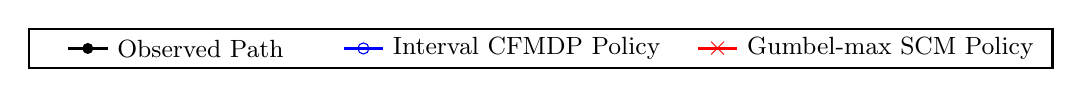
\begin{tikzpicture}[scale=1.0, every node/.style={scale=1.0}]
            \draw[thick, black] (-3, -0.25) rectangle (10, 0.25);
            %
            \draw[black, line width=1pt] (-2.5, 0.0) -- (-2,0.0);
            \fill[black] (-2.25,0.0) circle (2pt); %
            \node[right] at (-2,0.0) {\small Observed Path};
            
            %
            \draw[blue, line width=1pt] (1.0,0.0) -- (1.5,0.0);
            \node[draw=blue, circle, minimum size=4pt, inner sep=0pt] at (1.25,0.0) {}; %
            \node[right] at (1.5,0.0) {\small Interval CFMDP Policy};
            
            %
            \draw[red, line width=1pt] (5.5,0) -- (6,0);
            \node[red] at (5.75,0) {$\boldsymbol{\times}$}; %
            \node[right] at (6,0) {\small Gumbel-max SCM Policy};
        \end{tikzpicture}
    }\\
    %
    \subfigure[\footnotesize Lowest cumulative reward: Interval CFMDP ($312$), Gumbel-max SCM ($312$)]{%
        \resizebox{0.76\columnwidth}{!}{
             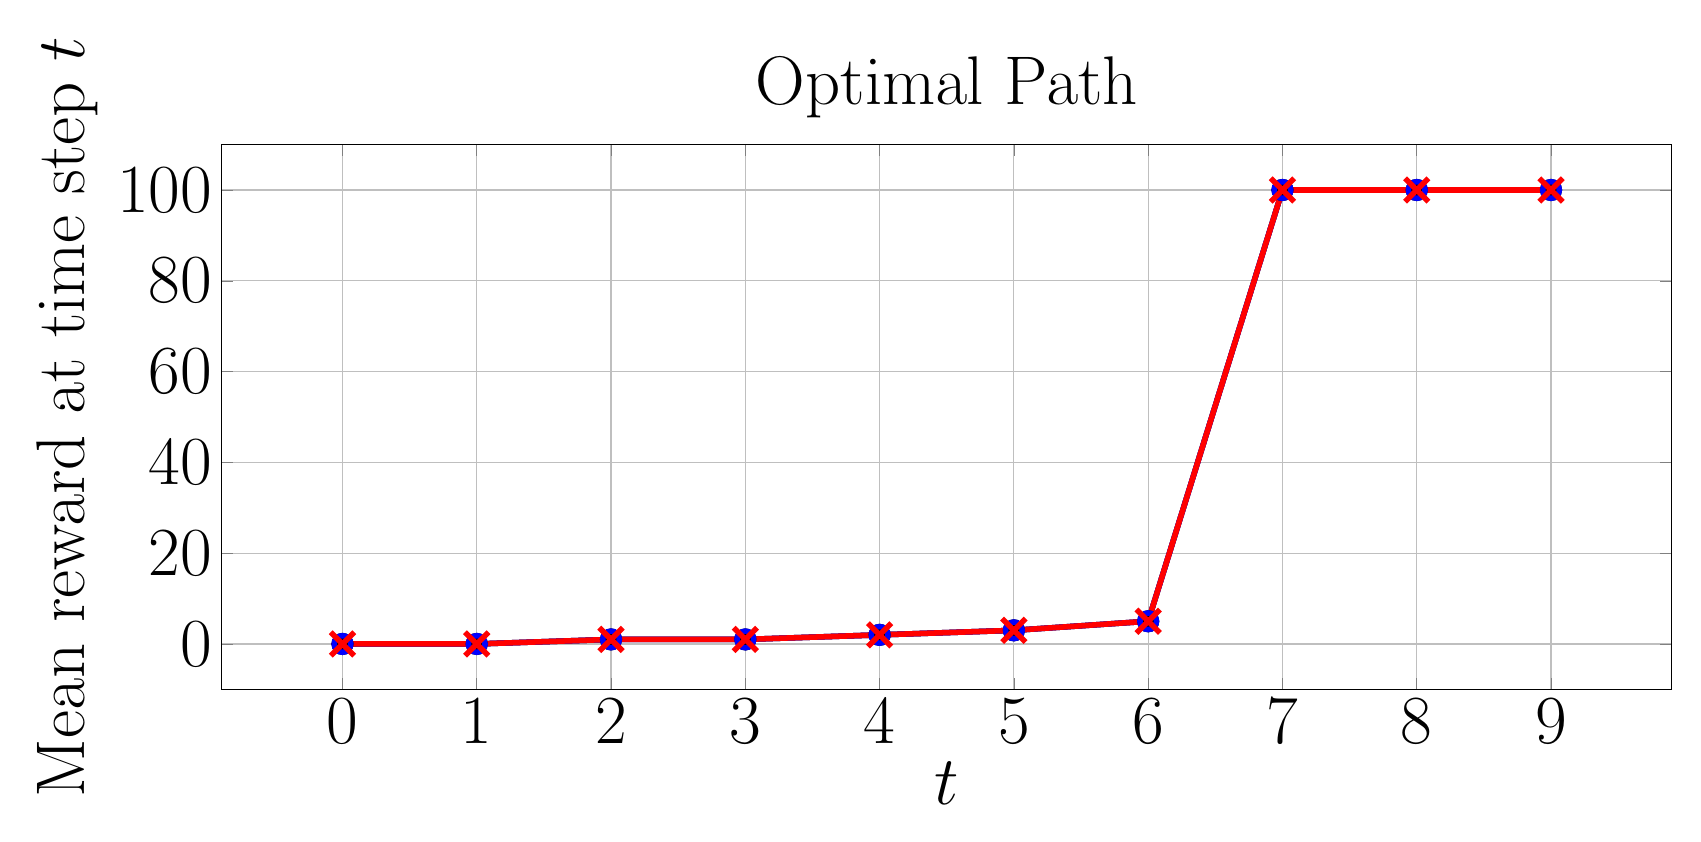
\begin{tikzpicture}
                \begin{axis}[
                    xlabel={$t$},
                    ylabel={Mean reward at time step $t$},
                    title={Optimal Path},
                    grid=both,
                    width=20cm, height=8.5cm,
                    every axis/.style={font=\Huge},
                    %
                ]
                \addplot[
                    color=black, %
                    mark=*, %
                    line width=2pt,
                    mark size=3pt,
                    error bars/.cd,
                    y dir=both, %
                    y explicit, %
                    error bar style={line width=1pt,solid},
                    error mark options={line width=1pt,mark size=4pt,rotate=90}
                ]
                coordinates {
                    (0, 0.0)  +- (0, 0.0)
                    (1, 0.0)  +- (0, 0.0) 
                    (2, 1.0)  +- (0, 0.0) 
                    (3, 1.0)  +- (0, 0.0)
                    (4, 2.0)  +- (0, 0.0)
                    (5, 3.0) +- (0, 0.0)
                    (6, 5.0) +- (0, 0.0)
                    (7, 100.0) +- (0, 0.0)
                    (8, 100.0) +- (0, 0.0)
                    (9, 100.0) +- (0, 0.0)
                };
                %
                \addplot[
                    color=blue, %
                    mark=o, %
                    line width=2pt,
                    mark size=3pt,
                    error bars/.cd,
                    y dir=both, %
                    y explicit, %
                    error bar style={line width=1pt,solid},
                    error mark options={line width=1pt,mark size=4pt,rotate=90}
                ]
                 coordinates {
                    (0, 0.0)  +- (0, 0.0)
                    (1, 0.0)  +- (0, 0.0) 
                    (2, 1.0)  +- (0, 0.0) 
                    (3, 1.0)  +- (0, 0.0)
                    (4, 2.0)  +- (0, 0.0)
                    (5, 3.0) +- (0, 0.0)
                    (6, 5.0) +- (0, 0.0)
                    (7, 100.0) +- (0, 0.0)
                    (8, 100.0) +- (0, 0.0)
                    (9, 100.0) +- (0, 0.0)
                };
                %
                \addplot[
                    color=red, %
                    mark=x, %
                    line width=2pt,
                    mark size=6pt,
                    error bars/.cd,
                    y dir=both, %
                    y explicit, %
                    error bar style={line width=1pt,solid},
                    error mark options={line width=1pt,mark size=4pt,rotate=90}
                ]
                coordinates {
                    (0, 0.0)  +- (0, 0.0)
                    (1, 0.0)  +- (0, 0.0) 
                    (2, 1.0)  +- (0, 0.0) 
                    (3, 1.0)  +- (0, 0.0)
                    (4, 2.0)  +- (0, 0.0)
                    (5, 3.0) +- (0, 0.0)
                    (6, 5.0) +- (0, 0.0)
                    (7, 100.0) +- (0, 0.0)
                    (8, 100.0) +- (0, 0.0)
                    (9, 100.0) +- (0, 0.0)
                };
                \end{axis}
            \end{tikzpicture}
         }
    }
    \hspace{1cm}
    \subfigure[\footnotesize Lowest cumulative reward: Interval CFMDP ($19$), Gumbel-max SCM ($-88$)]{%
         \resizebox{0.76\columnwidth}{!}{
            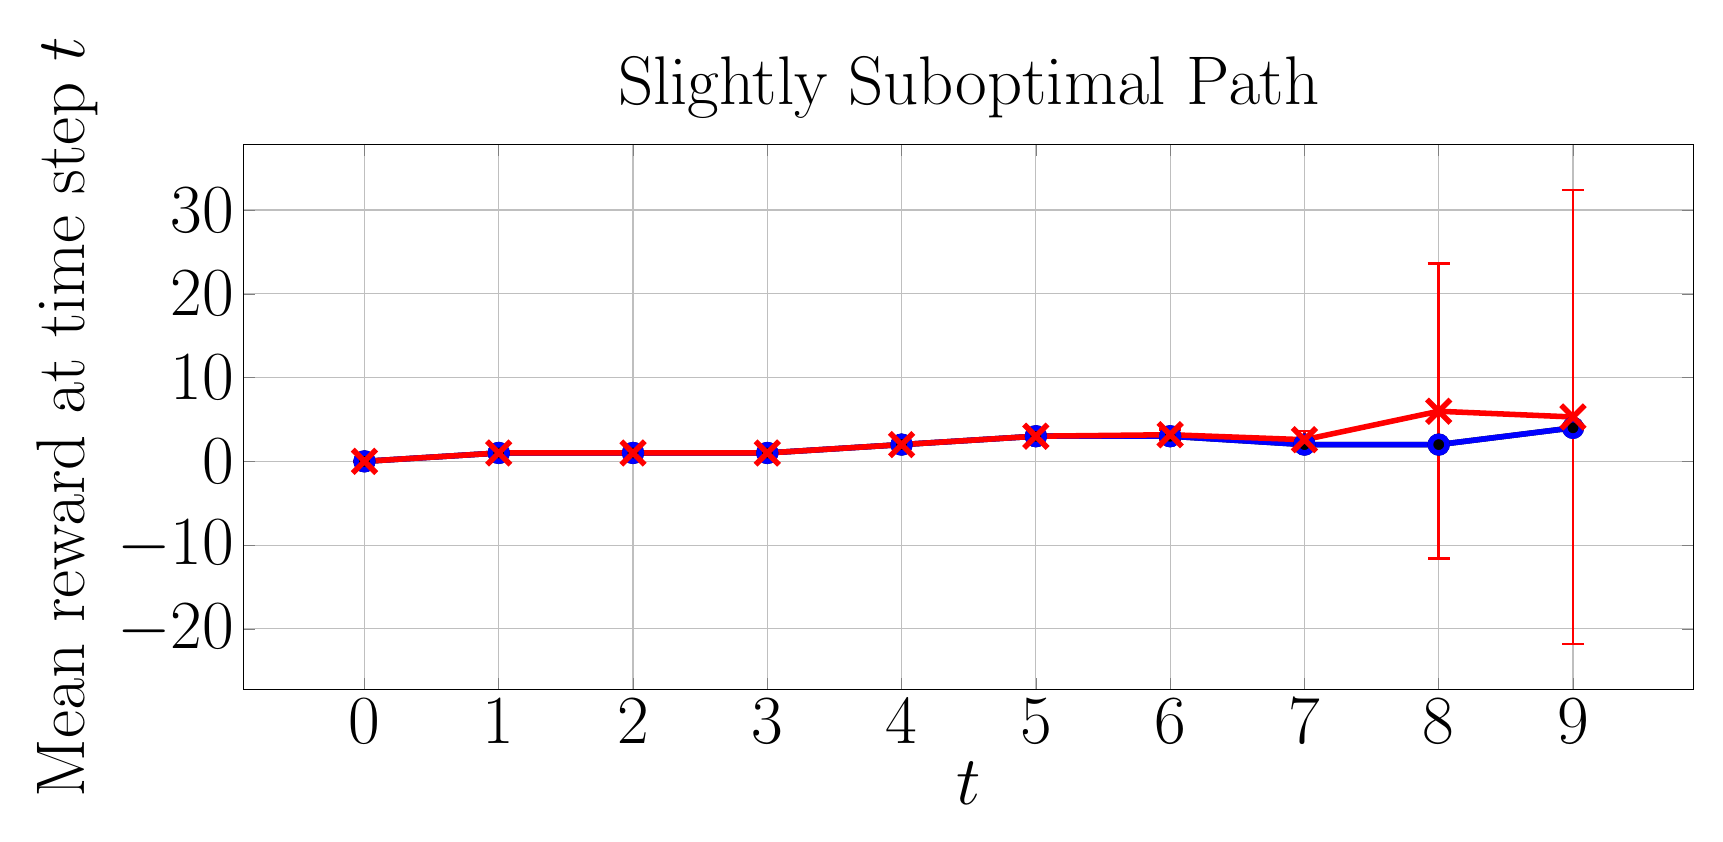
\begin{tikzpicture}
                \begin{axis}[
                    xlabel={$t$},
                    ylabel={Mean reward at time step $t$},
                    title={Slightly Suboptimal Path},
                    grid=both,
                    width=20cm, height=8.5cm,
                    every axis/.style={font=\Huge},
                    %
                ]
                \addplot[
                    color=black, %
                    mark=*, %
                    line width=2pt,
                    mark size=3pt,
                    error bars/.cd,
                    y dir=both, %
                    y explicit, %
                    error bar style={line width=1pt,solid},
                    error mark options={line width=1pt,mark size=4pt,rotate=90}
                ]
              coordinates {
                    (0, 0.0)  +- (0, 0.0)
                    (1, 1.0)  +- (0, 0.0) 
                    (2, 1.0)  +- (0, 0.0) 
                    (3, 1.0)  +- (0, 0.0)
                    (4, 2.0)  +- (0, 0.0)
                    (5, 3.0) +- (0, 0.0)
                    (6, 3.0) +- (0, 0.0)
                    (7, 2.0) +- (0, 0.0)
                    (8, 2.0) +- (0, 0.0)
                    (9, 4.0) +- (0, 0.0)
                };
                %
                \addplot[
                    color=blue, %
                    mark=o, %
                    line width=2pt,
                    mark size=3pt,
                    error bars/.cd,
                    y dir=both, %
                    y explicit, %
                    error bar style={line width=1pt,solid},
                    error mark options={line width=1pt,mark size=4pt,rotate=90}
                ]
              coordinates {
                    (0, 0.0)  +- (0, 0.0)
                    (1, 1.0)  +- (0, 0.0) 
                    (2, 1.0)  +- (0, 0.0) 
                    (3, 1.0)  +- (0, 0.0)
                    (4, 2.0)  +- (0, 0.0)
                    (5, 3.0) +- (0, 0.0)
                    (6, 3.0) +- (0, 0.0)
                    (7, 2.0) +- (0, 0.0)
                    (8, 2.0) +- (0, 0.0)
                    (9, 4.0) +- (0, 0.0)
                };
                %
                \addplot[
                    color=red, %
                    mark=x, %
                    line width=2pt,
                    mark size=6pt,
                    error bars/.cd,
                    y dir=both, %
                    y explicit, %
                    error bar style={line width=1pt,solid},
                    error mark options={line width=1pt,mark size=4pt,rotate=90}
                ]
                coordinates {
                    (0, 0.0)  +- (0, 0.0)
                    (1, 1.0)  +- (0, 0.0) 
                    (2, 1.0)  +- (0, 0.0) 
                    (3, 1.0)  +- (0, 0.0)
                    (4, 2.0)  += (0, 0.0)
                    (5, 3.0)  += (0, 0.0)
                    (6, 3.17847) += (0, 0.62606746) -= (0, 0.62606746)
                    (7, 2.5832885) += (0, 1.04598233) -= (0, 1.04598233)
                    (8, 5.978909) += (0, 17.60137623) -= (0, 17.60137623)
                    (9, 5.297059) += (0, 27.09227512) -= (0, 27.09227512)
                };
                \end{axis}
            \end{tikzpicture}
         }
    }\\[-1.5pt]
    \subfigure[\footnotesize Lowest cumulative reward: Interval CFMDP ($14$), Gumbel-max SCM ($-598$)]{%
         \resizebox{0.76\columnwidth}{!}{
             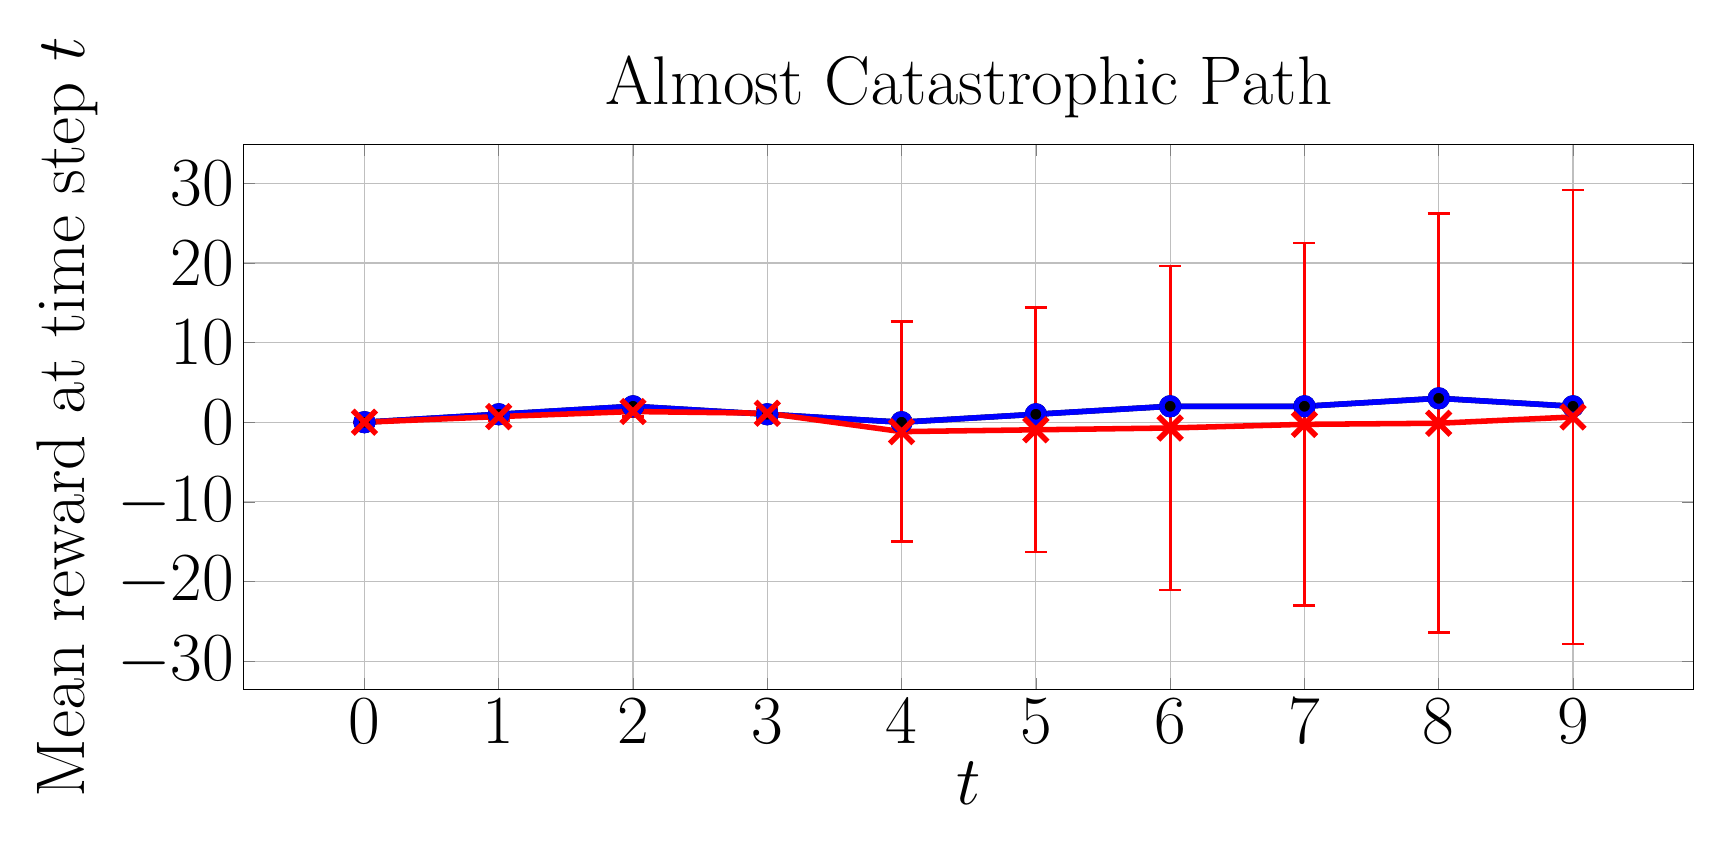
\begin{tikzpicture}
                \begin{axis}[
                    xlabel={$t$},
                    ylabel={Mean reward at time step $t$},
                    title={Almost Catastrophic Path},
                    grid=both,
                    width=20cm, height=8.5cm,
                    every axis/.style={font=\Huge},
                    %
                ]
                \addplot[
                    color=black, %
                    mark=*, %
                    line width=2pt,
                    mark size=3pt,
                    error bars/.cd,
                    y dir=both, %
                    y explicit, %
                    error bar style={line width=1pt,solid},
                    error mark options={line width=1pt,mark size=4pt,rotate=90}
                ]
                coordinates {
                    (0, 0.0)  +- (0, 0.0)
                    (1, 1.0)  +- (0, 0.0) 
                    (2, 2.0)  +- (0, 0.0) 
                    (3, 1.0)  +- (0, 0.0)
                    (4, 0.0)  +- (0, 0.0)
                    (5, 1.0) +- (0, 0.0)
                    (6, 2.0) +- (0, 0.0)
                    (7, 2.0) +- (0, 0.0)
                    (8, 3.0) +- (0, 0.0)
                    (9, 2.0) +- (0, 0.0)
                };
                %
                \addplot[
                    color=blue, %
                    mark=o, %
                    line width=2pt,
                    mark size=3pt,
                    error bars/.cd,
                    y dir=both, %
                    y explicit, %
                    error bar style={line width=1pt,solid},
                    error mark options={line width=1pt,mark size=4pt,rotate=90}
                ]
                coordinates {
                    (0, 0.0)  +- (0, 0.0)
                    (1, 1.0)  +- (0, 0.0) 
                    (2, 2.0)  +- (0, 0.0) 
                    (3, 1.0)  +- (0, 0.0)
                    (4, 0.0)  +- (0, 0.0)
                    (5, 1.0) +- (0, 0.0)
                    (6, 2.0) +- (0, 0.0)
                    (7, 2.0) +- (0, 0.0)
                    (8, 3.0) +- (0, 0.0)
                    (9, 2.0) +- (0, 0.0)
                };
                %
                \addplot[
                    color=red, %
                    mark=x, %
                    line width=2pt,
                    mark size=6pt,
                    error bars/.cd,
                    y dir=both, %
                    y explicit, %
                    error bar style={line width=1pt,solid},
                    error mark options={line width=1pt,mark size=4pt,rotate=90}
                ]
                coordinates {
                    (0, 0.0)  +- (0, 0.0)
                    (1, 0.7065655)  +- (0, 0.4553358) 
                    (2, 1.341673)  +- (0, 0.67091621) 
                    (3, 1.122926)  +- (0, 0.61281824)
                    (4, -1.1821935)  +- (0, 13.82444042)
                    (5, -0.952399)  +- (0, 15.35195457)
                    (6, -0.72672) +- (0, 20.33508414)
                    (7, -0.268983) +- (0, 22.77861454)
                    (8, -0.1310835) +- (0, 26.31013314)
                    (9, 0.65806) +- (0, 28.50670214)
                };
                %
            %
            %
            %
            %
            %
            %
            %
            %
            %
            %
            %
            %
            %
            %
            %
            %
            %
            %
                \end{axis}
            \end{tikzpicture}
         }
    }
    \hspace{1cm}
    \subfigure[\footnotesize Lowest cumulative reward: Interval CFMDP ($-698$), Gumbel-max SCM ($-698$)]{%
         \resizebox{0.76\columnwidth}{!}{
            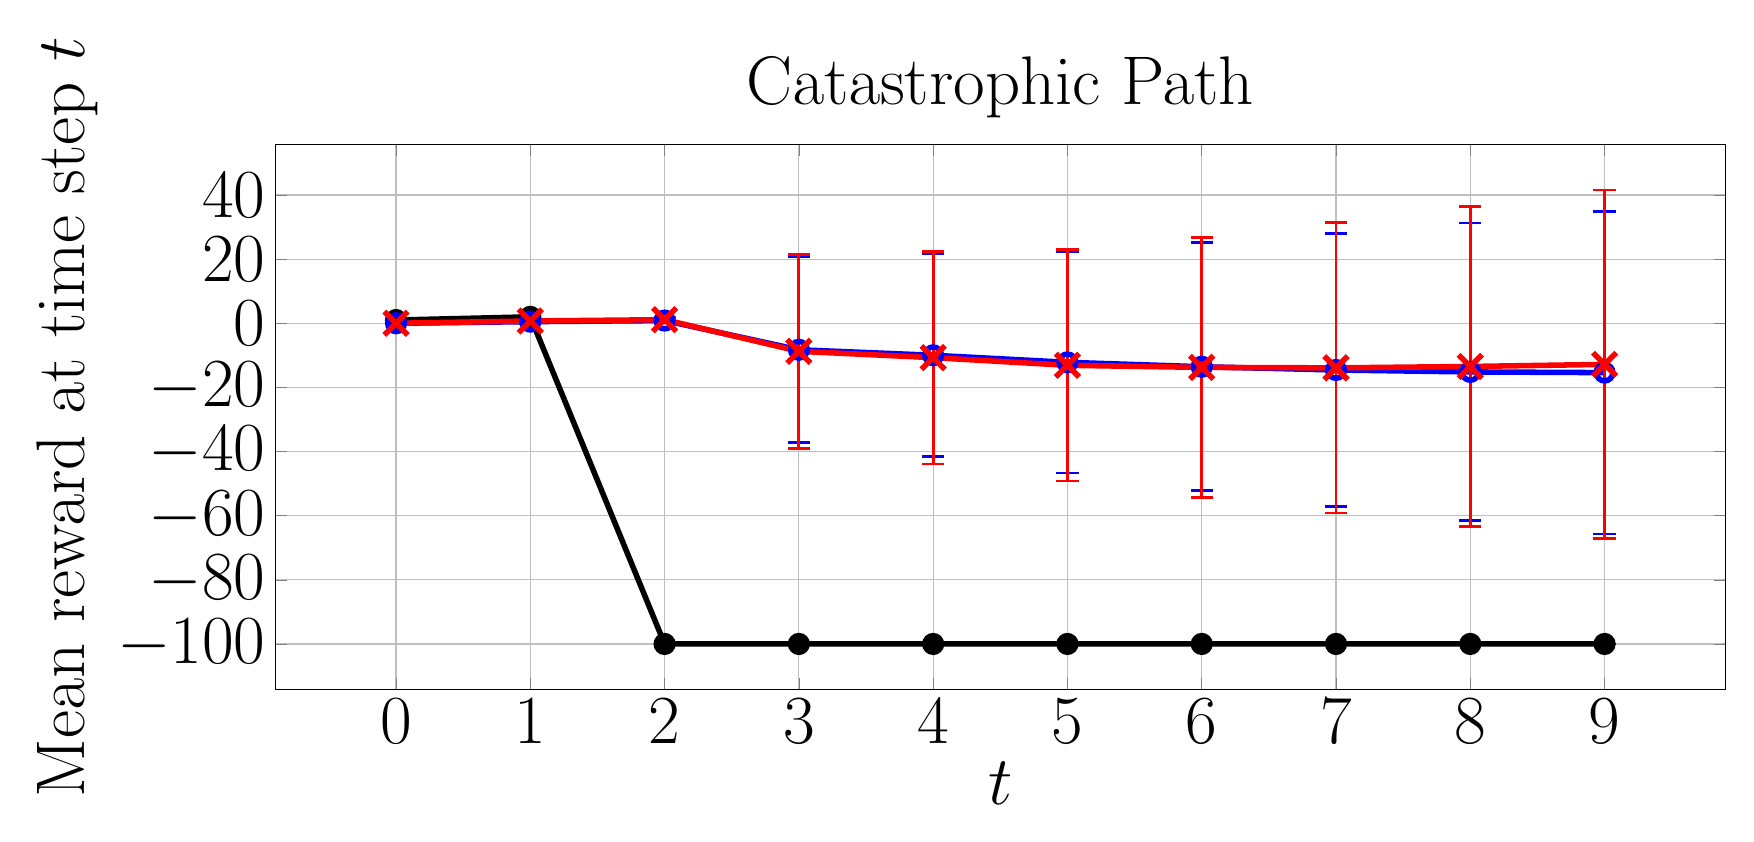
\begin{tikzpicture}
                \begin{axis}[
                    xlabel={$t$},
                    ylabel={Mean reward at time step $t$},
                    title={Catastrophic Path},
                    grid=both,
                    width=20cm, height=8.5cm,
                    every axis/.style={font=\Huge},
                    %
                ]
                \addplot[
                    color=black, %
                    mark=*, %
                    line width=2pt,
                    mark size=3pt,
                    error bars/.cd,
                    y dir=both, %
                    y explicit, %
                    error bar style={line width=1pt,solid},
                    error mark options={line width=1pt,mark size=4pt,rotate=90}
                ]
                coordinates {
                    (0, 1.0)  +- (0, 0.0)
                    (1, 2.0)  +- (0, 0.0) 
                    (2, -100.0)  +- (0, 0.0) 
                    (3, -100.0)  +- (0, 0.0)
                    (4, -100.0)  +- (0, 0.0)
                    (5, -100.0) +- (0, 0.0)
                    (6, -100.0) +- (0, 0.0)
                    (7, -100.0) +- (0, 0.0)
                    (8, -100.0) +- (0, 0.0)
                    (9, -100.0) +- (0, 0.0)
                };
                %
                \addplot[
                    color=blue, %
                    mark=o, %
                    line width=2pt,
                    mark size=3pt,
                    error bars/.cd,
                    y dir=both, %
                    y explicit, %
                    error bar style={line width=1pt,solid},
                    error mark options={line width=1pt,mark size=4pt,rotate=90}
                ]
                coordinates {
                    (0, 0.0)  +- (0, 0.0)
                    (1, 0.504814)  +- (0, 0.49997682) 
                    (2, 0.8439835)  +- (0, 0.76831917) 
                    (3, -8.2709165)  +- (0, 28.93656754)
                    (4, -9.981082)  +- (0, 31.66825363)
                    (5, -12.1776325) +- (0, 34.53463233)
                    (6, -13.556076) +- (0, 38.62845372)
                    (7, -14.574418) +- (0, 42.49603359)
                    (8, -15.1757075) +- (0, 46.41913968)
                    (9, -15.3900395) +- (0, 50.33563368)
                };
                %
                \addplot[
                    color=red, %
                    mark=x, %
                    line width=2pt,
                    mark size=6pt,
                    error bars/.cd,
                    y dir=both, %
                    y explicit, %
                    error bar style={line width=1pt,solid},
                    error mark options={line width=1pt,mark size=4pt,rotate=90}
                ]
                coordinates {
                    (0, 0.0)  +- (0, 0.0)
                    (1, 0.701873)  +- (0, 0.45743556) 
                    (2, 1.1227805)  +- (0, 0.73433129) 
                    (3, -8.7503255)  +- (0, 30.30257976)
                    (4, -10.722092)  +- (0, 33.17618589)
                    (5, -13.10721)  +- (0, 36.0648089)
                    (6, -13.7631645) +- (0, 40.56553451)
                    (7, -13.909043) +- (0, 45.23829402)
                    (8, -13.472517) +- (0, 49.96270296)
                    (9, -12.8278835) +- (0, 54.38618735)
                };
                %
            %
            %
            %
            %
            %
            %
            %
            %
            %
            %
            %
            %
            %
            %
            %
            %
            %
            %
                \end{axis}
            \end{tikzpicture}
         }
    }
    \caption{Average instant reward of CF paths induced by policies on GridWorld $p=0.4$.}
    \label{fig: reward p=0.4}
\end{figure*}

\subsection{Experimental Setup}
To compare policy performance, we measure the average rewards of counterfactual paths induced by our policy and the Gumbel-max policy by uniformly sampling $200$ counterfactual MDPs from the ICFMDP and generating $10,000$ counterfactual paths over each sampled CFMDP. \jl{Since the interval CFMDP depends on the observed path, we select $4$  paths of varying optimality to evaluate how the observed path impacts the performance of both policies: an optimal path, a slightly suboptimal path that could reach the optimal reward with a few changes, a catastrophic path that enters a catastrophic, terminal state with low reward, and an almost catastrophic path that was close to entering a catastrophic state.} When measuring the average probability bound widths and execution time needed to generate the ICFMDPs, we averaged over $20$ randomly generated observed paths
\footnote{Further training details are provided in Appendix \ref{app: training details}, and the code is provided at \href{https://github.com/ddv-lab/robust-cf-inference-in-MDPs}{https://github.com/ddv-lab/robust-cf-inference-in-MDPs}
%
%
.}.

\subsection{GridWorld}
\jl{The GridWorld MDP is a $4 \times 4$ grid where an agent must navigate from the top-left corner to the goal state in the bottom-right corner, avoiding a dangerous terminal state in the centre. At each time step, the agent can move up, down, left, or right, but there is a small probability (controlled by hyper-parameter $p$) of moving in an unintended direction. As the agent nears the goal, the reward for each state increases, culminating in a reward of $+100$ for reaching the goal. Entering the dangerous state results in a penalty of $-100$. We use two versions of GridWorld: a less stochastic version with $p=0.9$ (i.e., $90$\% chance of moving in the chosen direction) and a more stochastic version with $p=0.4$.}

\paragraph{GridWorld ($p=0.9$)}
When $p=0.9$, the counterfactual probability bounds are typically narrow (see Table \ref{tab:nonzero_probs} for average measurements). Consequently, as shown in Figure \ref{fig: reward p=0.9}, both policies are nearly identical and perform similarly well across the optimal, slightly suboptimal, and catastrophic paths.
%
However, for the almost catastrophic path, the interval CFMDP path is more conservative and follows the observed path more closely (as this is where the probability bounds are narrowest), which typically requires one additional step to reach the goal state than the Gumbel-max SCM policy.
%

\paragraph{GridWorld ($p=0.4$)}
\jl{When $p=0.4$, the GridWorld environment becomes more uncertain, increasing the risk of entering the dangerous state even if correct actions are chosen. Thus, as shown in Figure \ref{fig: reward p=0.4}, the interval CFMDP policy adopts a more conservative approach, avoiding deviation from the observed policy if it cannot guarantee higher counterfactual rewards (see the slightly suboptimal and almost catastrophic paths), whereas the Gumbel-max SCM is inconsistent: it can yield higher rewards, but also much lower rewards, reflected in the wide error bars.} For the catastrophic path, both policies must deviate from the observed path to achieve a higher reward and, in this case, perform similarly.
%
%
%
%
\subsection{Sepsis}
The Sepsis MDP \citep{oberst2019counterfactual} simulates trajectories of Sepsis patients. Each state consists of four vital signs (heart rate, blood pressure, oxygen concentration, and glucose levels), categorised as low, normal, or high.
and three treatments that can be toggled on/off at each time step (8 actions in total). Unlike \citet{oberst2019counterfactual}, we scale rewards based on the number of out-of-range vital signs, between $-1000$ (patient dies) and $1000$ (patient discharged). \jl{Like the GridWorld $p=0.4$ experiment, the Sepsis MDP is highly uncertain, as many states are equally likely to lead to optimal and poor outcomes. Thus, as shown in Figure \ref{fig: reward sepsis}, both policies follow the observed optimal and almost catastrophic paths to guarantee rewards are no worse than the observation.} However, improving the catastrophic path requires deviating from the observation. Here, the Gumbel-max SCM policy, on average, performs better than the interval CFMDP policy. But, since both policies have lower bounds clipped at $-1000$, neither policy reliably improves over the observation. In contrast, for the slightly suboptimal path, the interval CFMDP policy performs significantly better, shown by its higher lower bounds. 
Moreover, in these two cases, the worst-case counterfactual path generated by the interval CFMDP policy is better than that of the Gumbel-max SCM policy,
indicating its greater robustness.
%
\begin{figure*}
    \centering
     \resizebox{0.6\textwidth}{!}{
        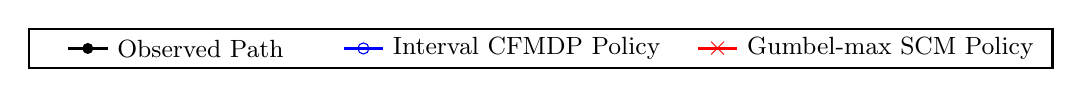
\begin{tikzpicture}[scale=1.0, every node/.style={scale=1.0}]
            \draw[thick, black] (-3, -0.25) rectangle (10, 0.25);
            %
            \draw[black, line width=1pt] (-2.5, 0.0) -- (-2,0.0);
            \fill[black] (-2.25,0.0) circle (2pt); %
            \node[right] at (-2,0.0) {\small Observed Path};
            
            %
            \draw[blue, line width=1pt] (1.0,0.0) -- (1.5,0.0);
            \node[draw=blue, circle, minimum size=4pt, inner sep=0pt] at (1.25,0.0) {}; %
            \node[right] at (1.5,0.0) {\small Interval CFMDP Policy};
            
            %
            \draw[red, line width=1pt] (5.5,0) -- (6,0);
            \node[red] at (5.75,0) {$\boldsymbol{\times}$}; %
            \node[right] at (6,0) {\small Gumbel-max SCM Policy};
        \end{tikzpicture}
    }\\
    \subfigure[\footnotesize Lowest cumulative reward: Interval CFMDP ($8000$), Gumbel-max SCM ($8000$)]{%
         \resizebox{0.76\columnwidth}{!}{
             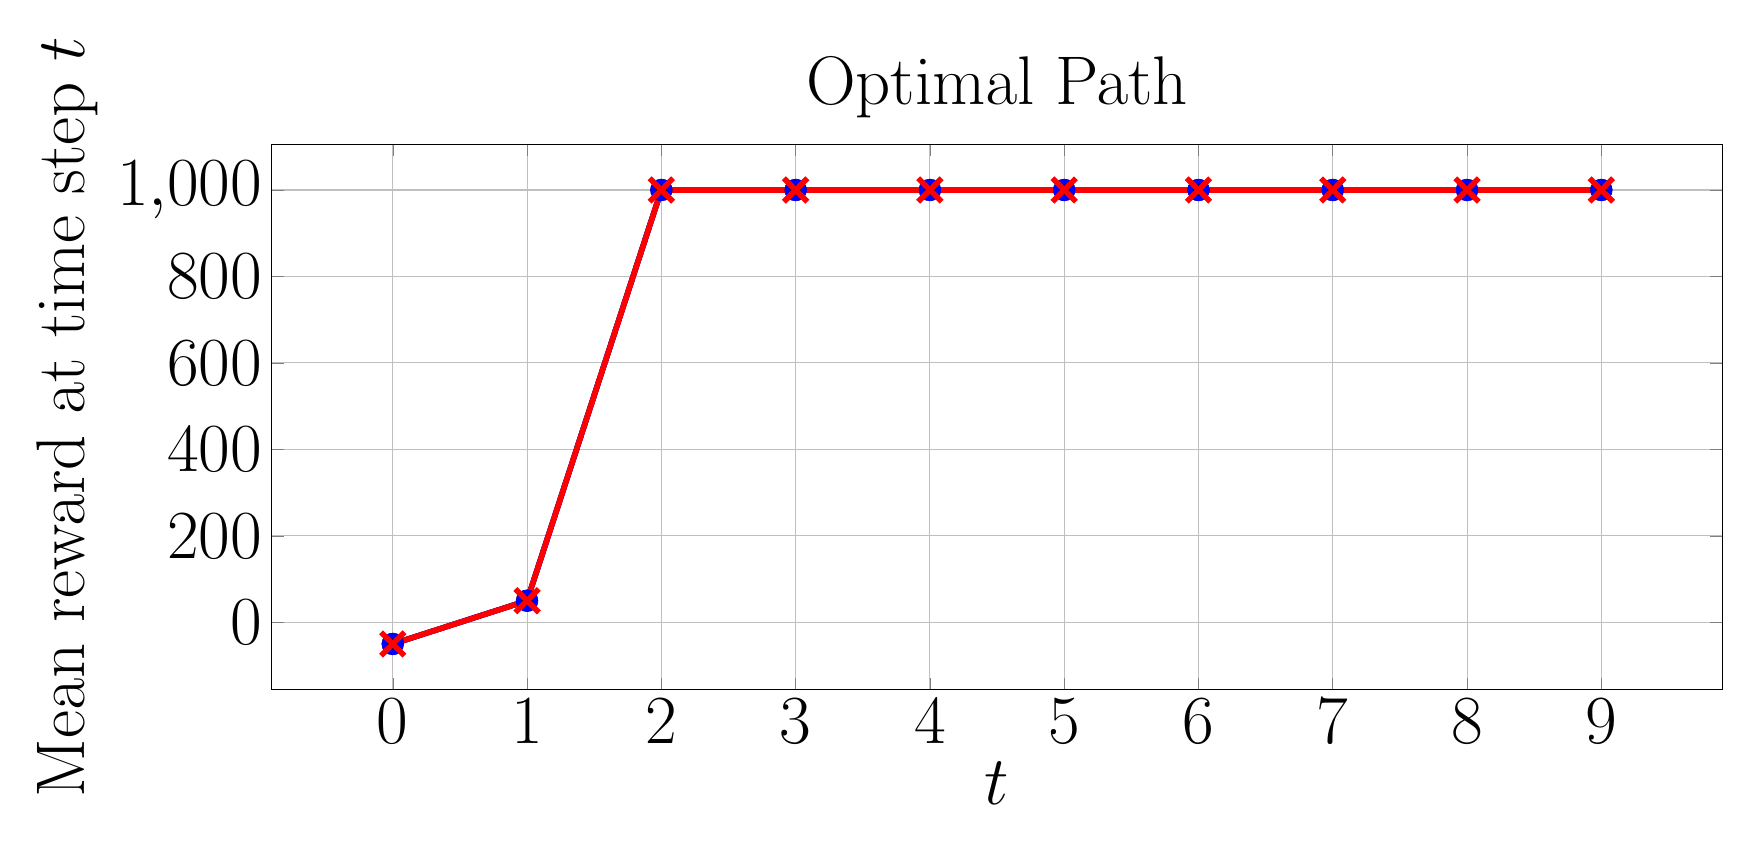
\begin{tikzpicture}
                \begin{axis}[
                    xlabel={$t$},
                    ylabel={Mean reward at time step $t$},
                    title={Optimal Path},
                    grid=both,
                    width=20cm, height=8.5cm,
                    every axis/.style={font=\Huge},
                    %
                ]
                \addplot[
                    color=black, %
                    mark=*, %
                    line width=2pt,
                    mark size=3pt,
                ]
                coordinates {
                    (0, -50.0)
                    (1, 50.0)
                    (2, 1000.0)
                    (3, 1000.0)
                    (4, 1000.0)
                    (5, 1000.0)
                    (6, 1000.0)
                    (7, 1000.0)
                    (8, 1000.0)
                    (9, 1000.0)
                };
                %
                \addplot[
                    color=blue, %
                    mark=o, %
                    line width=2pt,
                    mark size=3pt,
                    error bars/.cd,
                    y dir=both, %
                    y explicit, %
                    error bar style={line width=1pt,solid},
                    error mark options={line width=1pt,mark size=4pt,rotate=90}
                ]
                coordinates {
                    (0, -50.0)  +- (0, 0.0)
                    (1, 50.0)  +- (0, 0.0) 
                    (2, 1000.0)  +- (0, 0.0) 
                    (3, 1000.0)  +- (0, 0.0)
                    (4, 1000.0)  +- (0, 0.0)
                    (5, 1000.0) +- (0, 0.0)
                    (6, 1000.0) +- (0, 0.0)
                    (7, 1000.0) +- (0, 0.0)
                    (8, 1000.0) +- (0, 0.0)
                    (9, 1000.0) +- (0, 0.0)
                };
                %
                \addplot[
                    color=red, %
                    mark=x, %
                    line width=2pt,
                    mark size=6pt,
                    error bars/.cd,
                    y dir=both, %
                    y explicit, %
                    error bar style={line width=1pt,solid},
                    error mark options={line width=1pt,mark size=4pt,rotate=90}
                ]
                coordinates {
                    (0, -50.0)  +- (0, 0.0)
                    (1, 50.0)  +- (0, 0.0) 
                    (2, 1000.0)  +- (0, 0.0) 
                    (3, 1000.0)  +- (0, 0.0)
                    (4, 1000.0)  +- (0, 0.0)
                    (5, 1000.0) +- (0, 0.0)
                    (6, 1000.0) +- (0, 0.0)
                    (7, 1000.0) +- (0, 0.0)
                    (8, 1000.0) +- (0, 0.0)
                    (9, 1000.0) +- (0, 0.0)
                };
                %
                \end{axis}
            \end{tikzpicture}
         }
    }
    \hspace{1cm}
    \subfigure[\footnotesize Lowest cumulative reward: Interval CFMDP ($-5980$), Gumbel-max SCM ($-8000$)]{%
         \resizebox{0.76\columnwidth}{!}{
            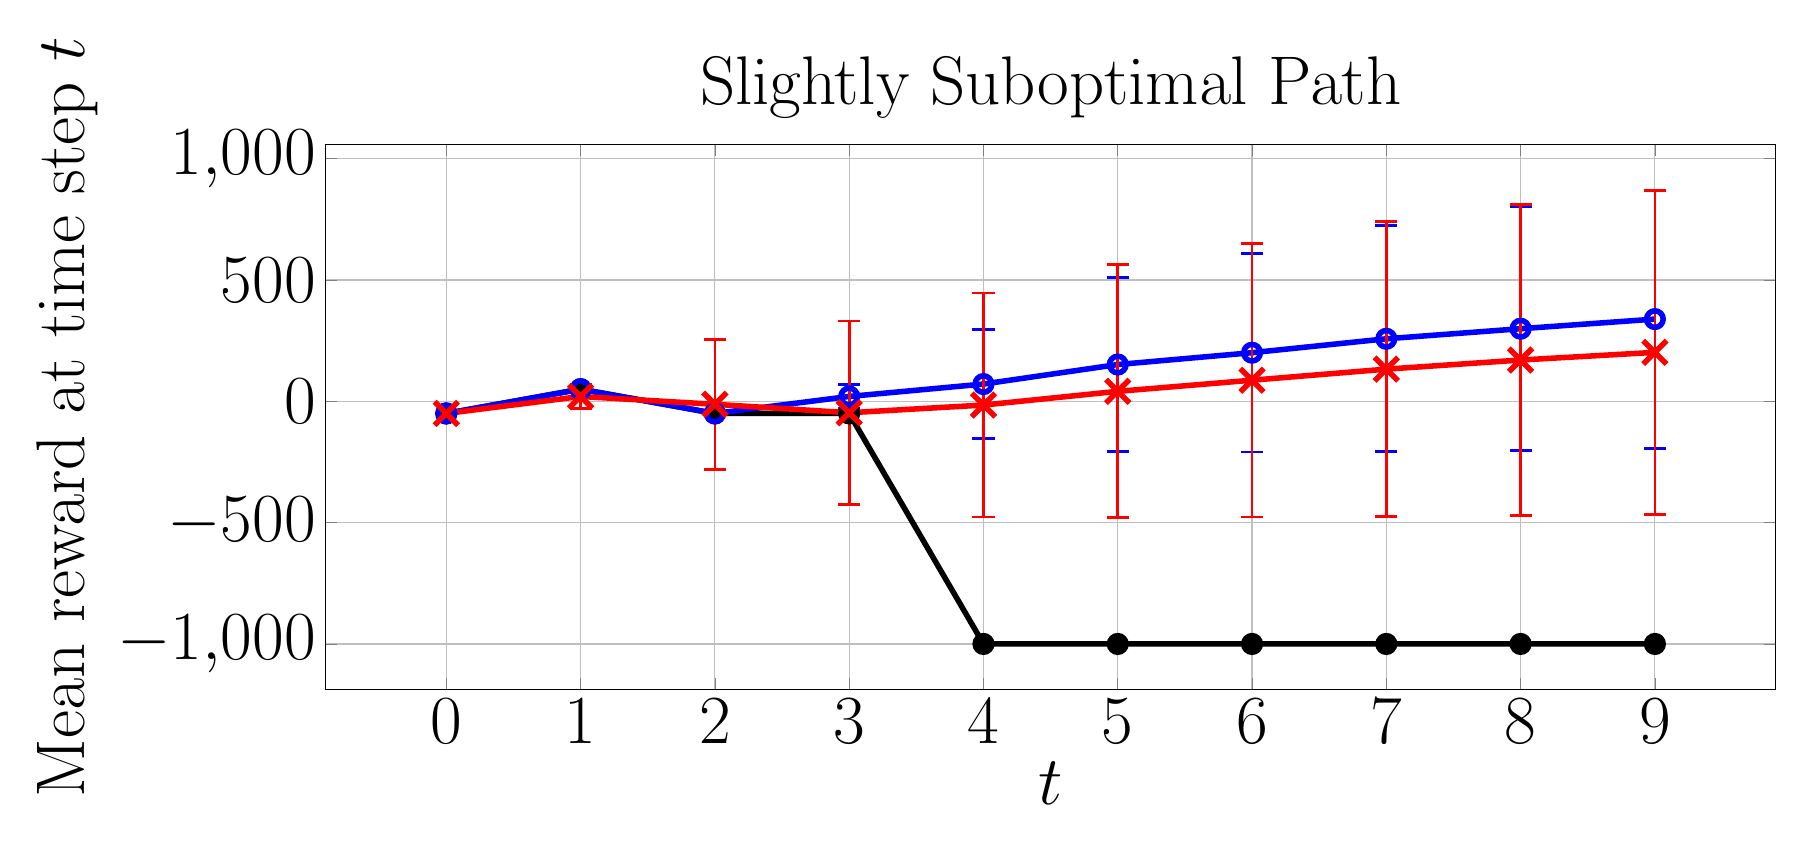
\begin{tikzpicture}
                \begin{axis}[
                    xlabel={$t$},
                    ylabel={Mean reward at time step $t$},
                    title={Slightly Suboptimal Path},
                    grid=both,
                    width=20cm, height=8.5cm,
                    every axis/.style={font=\Huge},
                    %
                ]
               \addplot[
                    color=black, %
                    mark=*, %
                    line width=2pt,
                    mark size=3pt,
                ]
                coordinates {
                    (0, -50.0)
                    (1, 50.0)
                    (2, -50.0)
                    (3, -50.0)
                    (4, -1000.0)
                    (5, -1000.0)
                    (6, -1000.0)
                    (7, -1000.0)
                    (8, -1000.0)
                    (9, -1000.0)
                };
                %
                \addplot[
                    color=blue, %
                    mark=o, %
                    line width=2pt,
                    mark size=3pt,
                    error bars/.cd,
                    y dir=both, %
                    y explicit, %
                    error bar style={line width=1pt,solid},
                    error mark options={line width=1pt,mark size=4pt,rotate=90}
                ]
                coordinates {
                    (0, -50.0)  +- (0, 0.0)
                    (1, 50.0)  +- (0, 0.0) 
                    (2, -50.0)  +- (0, 0.0) 
                    (3, 20.0631)  +- (0, 49.97539413)
                    (4, 71.206585)  +- (0, 226.02033693)
                    (5, 151.60797) +- (0, 359.23292559)
                    (6, 200.40593) +- (0, 408.86185176)
                    (7, 257.77948) +- (0, 466.10372804)
                    (8, 299.237465) +- (0, 501.82579506)
                    (9, 338.9129) +- (0, 532.06124996)
                };
                %
                \addplot[
                    color=red, %
                    mark=x, %
                    line width=2pt,
                    mark size=6pt,
                    error bars/.cd,
                    y dir=both, %
                    y explicit, %
                    error bar style={line width=1pt,solid},
                    error mark options={line width=1pt,mark size=4pt,rotate=90}
                ]
                coordinates {
                    (0, -50.0)  +- (0, 0.0)
                    (1, 20.00736)  +- (0, 49.99786741) 
                    (2, -12.282865)  +- (0, 267.598755) 
                    (3, -47.125995)  +- (0, 378.41755832)
                    (4, -15.381965)  +- (0, 461.77616558)
                    (5, 41.15459) +- (0, 521.53189262)
                    (6, 87.01595) +- (0, 564.22243126 )
                    (7, 132.62376) +- (0, 607.31338037)
                    (8, 170.168145) +- (0, 641.48013693)
                    (9, 201.813135) +- (0, 667.29441777)
                };
                %
                %
                %
                %
                %
                %
                %
                %
                %
                %
                %
                %
                %
                %
                %
                %
                %
                %
                %
                \end{axis}
            \end{tikzpicture}
         }
    }\\[-1.5pt]
    \subfigure[\footnotesize Lowest cumulative reward: Interval CFMDP ($100$), Gumbel-max SCM ($100$)]{%
         \resizebox{0.76\columnwidth}{!}{
             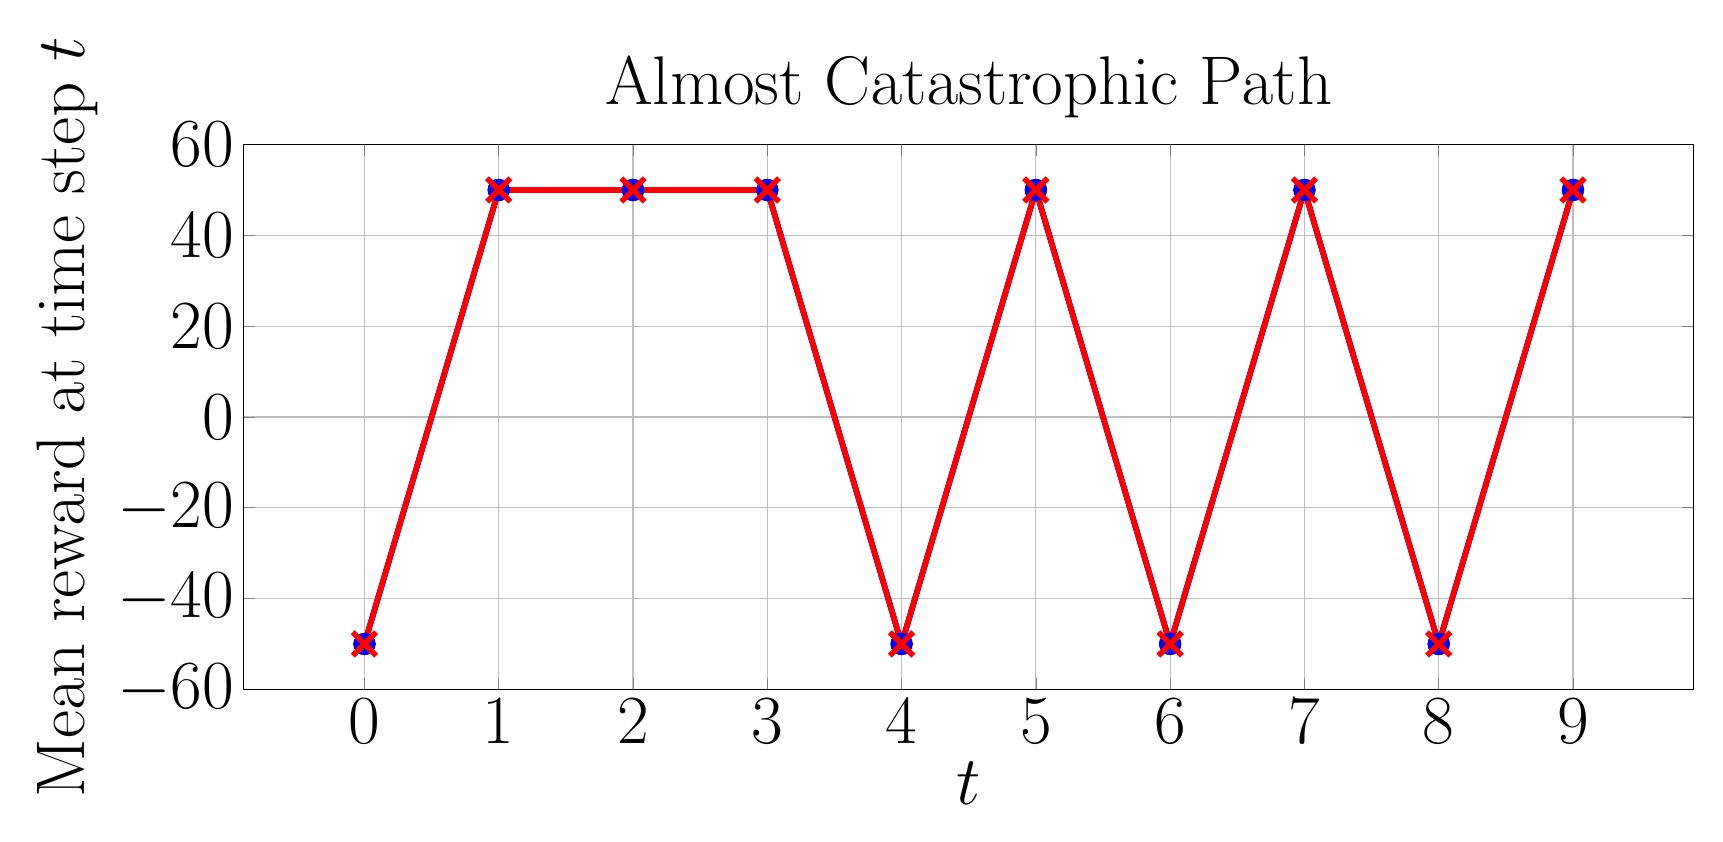
\begin{tikzpicture}
                \begin{axis}[
                    xlabel={$t$},
                    ylabel={Mean reward at time step $t$},
                    title={Almost Catastrophic Path},
                    grid=both,
                    every axis/.style={font=\Huge},
                    width=20cm, height=8.5cm,
                    %
                ]
               \addplot[
                    color=black, %
                    mark=*, %
                    line width=2pt,
                    mark size=3pt,
                ]
                coordinates {
                    (0, -50.0)
                    (1, 50.0)
                    (2, 50.0)
                    (3, 50.0)
                    (4, -50.0)
                    (5, 50.0)
                    (6, -50.0)
                    (7, 50.0)
                    (8, -50.0)
                    (9, 50.0)
                };
                %
                %
                \addplot[
                    color=blue, %
                    mark=o, %
                    line width=2pt,
                    mark size=3pt,
                    error bars/.cd,
                    y dir=both, %
                    y explicit, %
                    error bar style={line width=1pt,solid},
                    error mark options={line width=1pt,mark size=4pt,rotate=90}
                ]
                coordinates {
                    (0, -50.0)  +- (0, 0.0)
                    (1, 50.0)  +- (0, 0.0) 
                    (2, 50.0)  +- (0, 0.0) 
                    (3, 50.0)  +- (0, 0.0)
                    (4, -50.0)  +- (0, 0.0)
                    (5, 50.0) +- (0, 0.0)
                    (6, -50.0) +- (0, 0.0)
                    (7, 50.0) +- (0, 0.0)
                    (8, -50.0) +- (0, 0.0)
                    (9, 50.0) +- (0, 0.0)
                };
                %
                \addplot[
                    color=red, %
                    mark=x, %
                    line width=2pt,
                    mark size=6pt,
                    error bars/.cd,
                    y dir=both, %
                    y explicit, %
                    error bar style={line width=1pt,solid},
                    error mark options={line width=1pt,mark size=4pt,rotate=90}
                ]
                coordinates {
                    (0, -50.0)  +- (0, 0.0)
                    (1, 50.0)  +- (0, 0.0) 
                    (2, 50.0)  +- (0, 0.0) 
                    (3, 50.0)  +- (0, 0.0)
                    (4, -50.0)  +- (0, 0.0)
                    (5, 50.0) +- (0, 0.0)
                    (6, -50.0) +- (0, 0.0)
                    (7, 50.0) +- (0, 0.0)
                    (8, -50.0) +- (0, 0.0)
                    (9, 50.0) +- (0, 0.0)
                };
                %
                %
                %
                %
                %
                %
                %
                %
                %
                %
                %
                %
                %
                %
                %
                %
                %
                %
                %
                \end{axis}
            \end{tikzpicture}
         }
    }
    \hspace{1cm}
    \subfigure[\footnotesize Lowest cumulative reward: Interval CFMDP ($-7150$), Gumbel-max SCM ($-9050$)]{%
         \resizebox{0.76\columnwidth}{!}{
            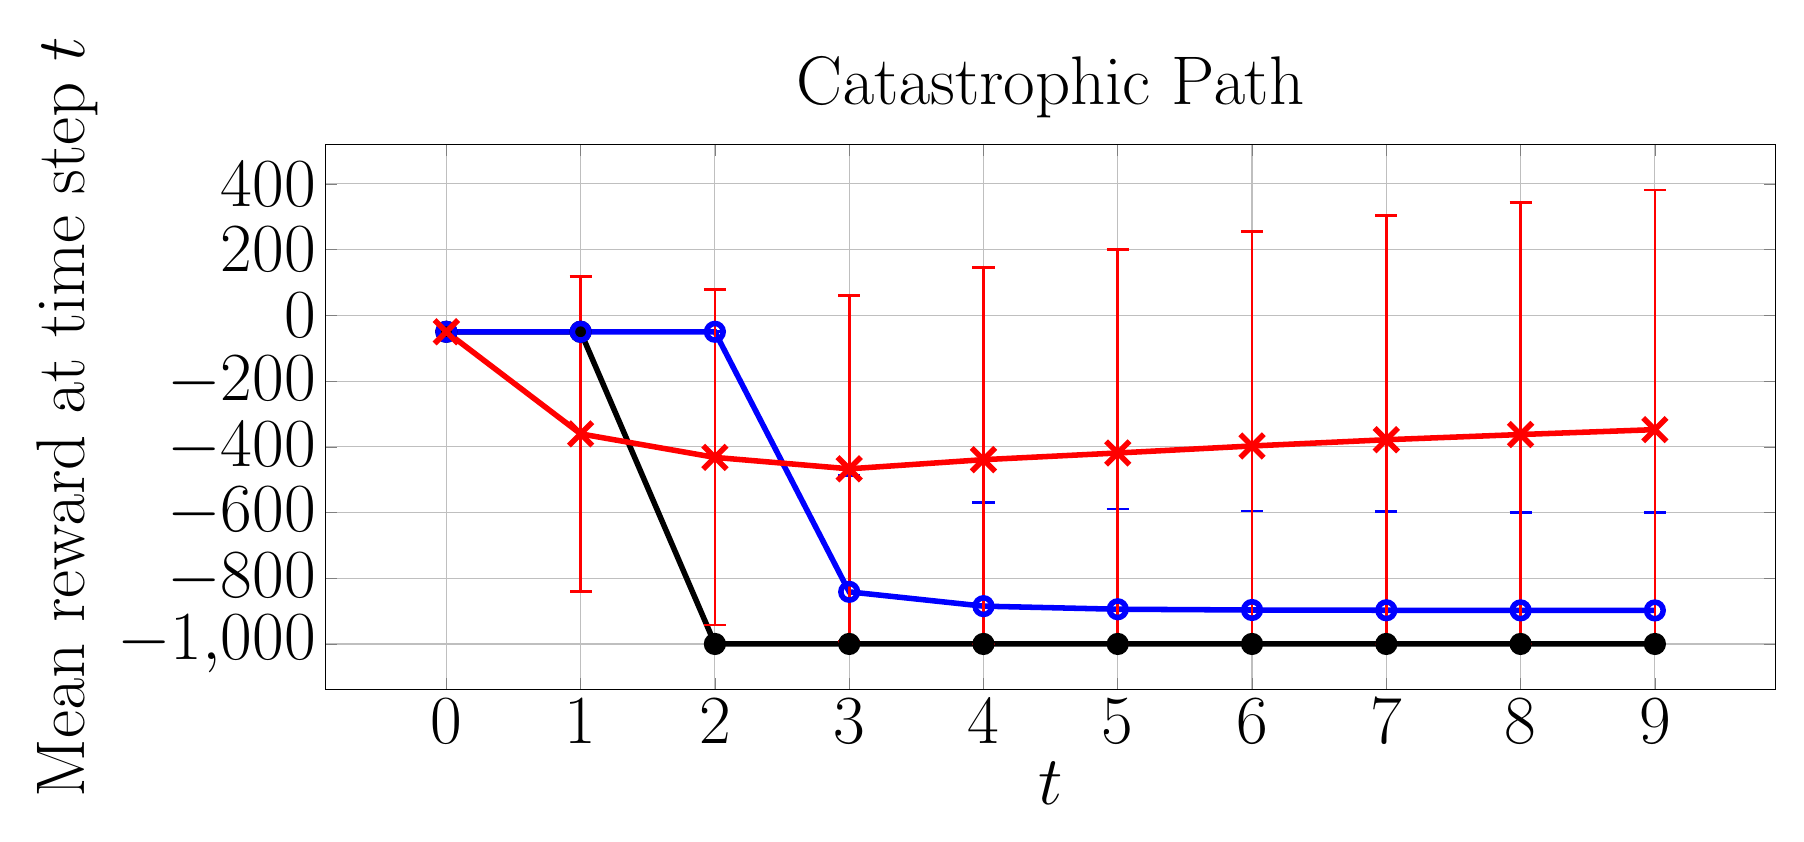
\begin{tikzpicture}
                \begin{axis}[
                    xlabel={$t$},
                    ylabel={Mean reward at time step $t$},
                    title={Catastrophic Path},
                    grid=both,
                    width=20cm, height=8.5cm,
                    every axis/.style={font=\Huge},
                    %
                ]
               \addplot[
                    color=black, %
                    mark=*, %
                    line width=2pt,
                    mark size=3pt,
                ]
                coordinates {
                    (0, -50.0)
                    (1, -50.0)
                    (2, -1000.0)
                    (3, -1000.0)
                    (4, -1000.0)
                    (5, -1000.0)
                    (6, -1000.0)
                    (7, -1000.0)
                    (8, -1000.0)
                    (9, -1000.0)
                };
                %
                %
                \addplot[
                    color=blue, %
                    mark=o, %
                    line width=2pt,
                    mark size=3pt,
                    error bars/.cd,
                    y dir=both, %
                    y explicit, %
                    error bar style={line width=1pt,solid},
                    error mark options={line width=1pt,mark size=4pt,rotate=90}
                ]
                coordinates {
                    (0, -50.0)  +- (0, 0.0)
                    (1, -50.0)  +- (0, 0.0) 
                    (2, -50.0)  +- (0, 0.0) 
                    (3, -841.440725)  += (0, 354.24605512) -= (0, 158.559275)
                    (4, -884.98225)  += (0, 315.37519669) -= (0, 115.01775)
                    (5, -894.330425) += (0, 304.88572805) -= (0, 105.669575)
                    (6, -896.696175) += (0, 301.19954514) -= (0, 103.303825)
                    (7, -897.4635) += (0, 299.61791279) -= (0, 102.5365)
                    (8, -897.77595) += (0, 298.80392585) -= (0, 102.22405)
                    (9, -897.942975) += (0, 298.32920557) -= (0, 102.057025)
                };
                %
                \addplot[
                    color=red, %
                    mark=x, %
                    line width=2pt,
                    mark size=6pt,
                    error bars/.cd,
                    y dir=both, %
                    y explicit, %
                    error bar style={line width=1pt,solid},
                    error mark options={line width=1pt,mark size=4pt,rotate=90}
                ]
            coordinates {
                    (0, -50.0)  +- (0, 0.0)
                    (1, -360.675265)  +- (0, 479.39812699) 
                    (2, -432.27629)  +- (0, 510.38620897) 
                    (3, -467.029545)  += (0, 526.36009628) -= (0, 526.36009628)
                    (4, -439.17429)  += (0, 583.96638919) -= (0, 560.82571)
                    (5, -418.82704) += (0, 618.43027478) -= (0, 581.17296)
                    (6, -397.464895) += (0, 652.67322574) -= (0, 602.535105)
                    (7, -378.49052) += (0, 682.85407033) -= (0, 621.50948)
                    (8, -362.654195) += (0, 707.01412023) -= (0, 637.345805)
                    (9, -347.737935) += (0, 729.29076479) -= (0, 652.262065)
                };
                %
                %
                %
                %
                %
                %
                %
                %
                %
                %
                %
                %
                %
                %
                %
                %
                %
                %
                %
                \end{axis}
            \end{tikzpicture}
         }
    }
    \caption{Average instant reward of CF paths induced by policies on Sepsis.}
    \label{fig: reward sepsis}
\end{figure*}

%
%
%
\subsection{Interval CFMDP Bounds}
%
%
Table \ref{tab:nonzero_probs} presents the mean counterfactual probability bound widths (excluding transitions where the upper bound is $0$) for each MDP, averaged over 20 observed paths. We compare the bounds under counterfactual stability (CS) and monotonicity (M) assumptions, CS alone, and no assumptions. This shows that the assumptions marginally reduce the bound widths, indicating the assumptions tighten the bounds without excluding too many causal models, as intended.
\renewcommand{\arraystretch}{1}

\begin{table}
\centering
\caption{Mean width of counterfactual probability bounds}
\resizebox{0.8\columnwidth}{!}{%
\begin{tabular}{|c|c|c|c|}
\hline
\multirow{2}{*}{\textbf{Environment}} & \multicolumn{3}{c|}{\textbf{Assumptions}} \\ \cline{2-4}
 & \textbf{CS + M} & \textbf{CS} & \textbf{None\tablefootnote{\jl{Equivalent to \citet{li2024probabilities}'s bounds (see Section \ref{sec: equivalence with Li}).}}} \\ \hline
\textbf{GridWorld} ($p=0.9$) & 0.0817 & 0.0977 & 0.100 \\ \hline
\textbf{GridWorld} ($p=0.4$) & 0.552  & 0.638  & 0.646 \\ \hline
\textbf{Sepsis} & 0.138 & 0.140 & 0.140 \\ \hline
\end{tabular}
}
\label{tab:nonzero_probs}
\end{table}


\subsection{Execution Times}
Table \ref{tab: times} compares the average time needed to generate the interval CFMDP vs.\ the Gumbel-max SCM CFMDP for 20 observations.
The GridWorld algorithms were run single-threaded, while the Sepsis experiments were run in parallel.
Generating the interval CFMDP is significantly faster as it uses exact analytical bounds, whereas the Gumbel-max CFMDP requires sampling from the Gumbel distribution to estimate counterfactual transition probabilities. \jl{Since constructing the counterfactual MDP models is the main bottleneck in both approaches, ours is more efficient overall and suitable for larger MDPs.}
\begin{table}
\centering
\caption{Mean execution time to generate CFMDPs}
\resizebox{0.99\columnwidth}{!}{%
\begin{tabular}{|c|c|c|}
\hline
\multirow{2}{*}{\textbf{Environment}} & \multicolumn{2}{c|}{\textbf{Mean Execution Time (s)}} \\ \cline{2-3} 
                                      & \textbf{Interval CFMDP} & \textbf{Gumbel-max CFMDP} \\ \hline
\textbf{GridWorld ($p=0.9$) }                  & 0.261                   & 56.1                      \\ \hline
\textbf{GridWorld ($p=0.4$)  }                 & 0.336                   & 54.5                      \\ \hline
\textbf{Sepsis}                                 & 688                     & 2940                      \\ \hline
\end{tabular}%
}
\label{tab: times}
\end{table}

\subsection{RQ3: Effectiveness of Search Strategies to Adapt Out-of-Scope Inputs. }

\textit{Baseline:} We employed two search strategies; namely random search (\textbf{CodeImprove-rand})~\cite{zabinsky2009random}, and Hill climbing algorithm (\textbf{CodeImprove-HC})~\cite{selman2006hill}. \textbf{CodeImprove-rand} \textcolor{blue}{applies} random transformations until identifying the optimal candidate. \textbf{CodeImprove-HC} \textcolor{blue}{follows} the principles of the hill climbing algorithm. 


\textit{Process:} For CodeImprove-rand, we randomly apply transformation operators until the algorithm finds the best candidate. CodeImprove-HC begins with an initial solution (i.e., obtained through a random transformation). Subsequently, it iteratively applies a single transformation operator to this solution while computing the fitness score. If the current solution surpasses the threshold for fitness score, the algorithm terminates, having achieved the optimal solution. To be fair, we set up a number of transformations for a solution to 15 in all the techniques. For CodeImprove, each candidate solution \textcolor{blue}{undergoes} all 15 operators during crossover. 

\textit{Results: } Table~\ref{Tab:evaluation} shows the comparison of the three approaches. From this table, we observe that: (1) CodeImprove obtained the best accuracy across all subjects (up to 8.78\%) while both CodeImprove-rand and CodeImprove-HC did not achieve the performance of CodeImprove (up to 2.13\%); (2) Although CodeImprove-HC and CodeImprove-rand improve the model performance, we find that these search algorithms stop at the local minima (i.e., once the algorithm identifies a better candidate, the process terminates). However, CodeImprove will evolve for multiple generations i.e., in our case, is three to find the best candidate; (3) In terms of correcting mispredictions CodeImprove performs the best (i.e.,  CSR up to 39.9\%); (4) Although CodeImprove-rand and CodeImprove-HC shows lower values of MCR, note that its CSR values are really low, therefore, unable to correct mispredictions in a large scale; and (5) In conclusion, CodeImprove is a stable approach to adapt program inputs.  

\begin{tcolorbox}[title=\textbf{RQ3} - How effective to convert out-of-scope data to become in-scope data?, left=2pt, right=2pt,top=2pt,bottom=2pt]
CodeImprove is better at correcting out-of-scope inputs compared to other search algorithms such as random search and hill climbing. 
\end{tcolorbox}



\subsection{RQ4: Influence of Hyper-parameters}
\section{Upper Bound for the Global Sensitivity of LZ77 Compression}\seclab{sec:upperbound}

Recall that in \secref{sec:dpcompress}, we provided the framework to convert any compression scheme to a $(\epsilon,\delta)$-DP compression scheme by adding a random amount of padding $p=\max\left\{1, \lceil Z+k\rceil \right\}$, where $Z\sim\Lap(\GS_\compress/\epsilon)$ and $k=\frac{\GS_\compress}{\epsilon}\ln(\frac{1}{2\delta})+\GS_\compress +1$ is a constant. We observed that as long as $k=o(n)$, we can still argue that $\dpcompress$ achieves efficient compression ratios, i.e., $\left| \dpcompress(w,\epsilon,\delta) \right|/ n = \left| \compress(w) \right|/ n + o(1)$. That was the motivation to find practical compression schemes with global sensitivity $o(n)$. We argue that the LZ77 compression scheme \cite{LZ77} satisfies this property. For simplicity of exposition, we will assume that $W=n$ in most of our analysis and then briefly explain how the analysis changes when $W < n$. In particular, we prove that the global sensitivity of the LZ77 compression scheme is $\O{W^{2/3}\log n}$ or $\O{n^{2/3}\log n}$ when $W=n$.

\subsection{Analyzing the Positions of Blocks}

Recall that the LZ77 compression algorithm \cite{LZ77} with the compression function $\compress:\Sigma^*\rightarrow(\Sigma')^*$ outputs a sequence of blocks $B_1,\ldots,B_t$ where each block is of the form $B_i=[q_i,\ell_i,c_i]$ such that $0\leq q_i,\ell_i< n$ are nonnegative integers and $c_i\in\Sigma$ is a character. This implies that for a string $w\in\Sigma^n$, it takes $2\lceil\log n\rceil + \lceil\log|\Sigma|\rceil$ bits to encode each block and this is the same for all the blocks. Therefore, the length of compression is proportional to the number of blocks $t$, i.e., we have $|\compress(w)| = t(2\lceil\log n\rceil + \lceil\log|\Sigma|\rceil)$. Let $B_1',\ldots, B_{t'}'$ denotes the blocks when compressing $w'$ instead of $w$. Our observation above tells us that to analyze the global sensitivity of the LZ77 compression scheme, it is crucial to understand the upper/lower bound of $t'-t$ (WLOG we can assume $t'\geq t$ since we can always change the role of $w$ and $w'$) where $t$ (resp. $t'$) is the number of blocks in $\compress(w)$ (resp. $\compress(w')$) for neighboring strings $w\sim w'\in\Sigma^n$.

To analyze the difference between the number of blocks $t'-t$, it is helpful to introduce some notation. First, since $w \sim w'$ we will use $j \leq n$ to denote the unique index such that $w[j] \neq w'[j]$ --- note that $w[i] = w'[i]$ for all $i \neq j$. Second, the block $B_i=[q_i,\ell_i,c_i]$ can be viewed intuitively as an instruction for the decompression algorithm to locate the substring $w[q_i,q_i+\ell_i-1]$ from the part of $w$ that we have already decompressed, copy this substring and append it to the end of the of the decompressed file followed by the character $c_i$. While the inputs $q_i$ and $\ell_i$ tell us where to copy {\em from} it is also useful to let $s_i \coloneqq 1+\sum_{j=1}^{i-1} (\ell_i +1)$ and $f_i \coloneqq \sum_{j=1}^{i} (\ell_i +1)$ denote the location where the block is copied {\em to}, i.e., we have $w[s_i,f_i]  = w[q_i,q_i+\ell_i-1] \circ c_i$. 

We say that block $B_k'$ starts inside block $B_i$ if $s_i\leq s_k'\leq f_i$ and we indicate this with the predicate  $\startinside(i,k)\coloneqq 1$. Otherwise, if $s_k' < s_i$ or $s_k' > f_i$ then we have  $\startinside(i,k)\coloneqq 0$. Our key technical insight is that if $\startinside(i,k)=1$ then for block $B_{k+1}'$ we must have $f_{k+1}' \geq f_k$. In particular, for later blocks $B'_{k'}$ with $k'>k$ we will have $s'_{k'} > f_i$ so $\startinside(i,k')=0$. In particular, if we let $\M_i \coloneqq \{ k \in [t']~:~\startinside(i,k)=1\}$ then   \lemref{lemma:start_inside} tells us that one of three cases applies: (1) $\M_i = \emptyset$, (2) $\M_i = \{k\}$ for some $k \leq t'$, or (3) $\M_i = \{k,k+1\}$ for some $k < t'$. In any case, we have $\left| \M_i \right| \leq 2$.

%$k \in [t']$ starts inside $$ 



%a predicate called $\startinside:\mathbb{Z}\times\mathbb{Z}\rightarrow\bin$ which tells us whether a specific block in $\compress(w')$ starts inside a specific block in $\compress(w)$ or not. Intuitively, given strings $w\sim w'\in\Sigma^n$ and outputs of the LZ77 compression $(B_1,\ldots,B_t)\gets\compress(w)$ and $(B'_1,\ldots,B'_{t'})\gets\compress(w')$, let $s_i$ and $f_i$ (resp. $s_k'$ and $f_k'$) be the start and end position of the block $B_i$ (resp. $B_k'$) for $i\in[t]$ (resp. $k\in[t']$). If $s_i\leq s_k'\leq f_i$, then we say that block $B_k'$ \emph{starts inside} block $B_i$ which we indicate with the predicate $\startinside(i,k)=1$. Otherwise, we define $\startinside(i,k)=0$.

%Our main insight is that if $B_k'$ starts inside $B_i$ then $f_{k+1}' \geq f_i$, i.e., block $B_{k+1}'$ cannot finish before $B_i$ and, .


%we define $\startinside(i,k)=1$ if and only if $B_k'$ \emph{starts inside} $B_i$ and $0$ otherwise. We say that $B_k'$ starts inside $B_i$ if the start position of $B_k'$ lies inside $B_i$; let $s_i$ and $f_i$ (resp. $s_k'$ and $f_k'$) be the start and end position of the block $B_i$ (resp. $B_k'$). Then $\startinside(i,k)=1$ if and only if the following conditions hold: (1) $1\leq i\leq t$, (2) $1\leq k\leq t'$, and $s_i\leq s_k'\leq f_i$.

%We prove that given strings $w\sim w'\in\Sigma^n$ and $(B_1,\ldots,B_t)\gets\compress(w)$ and $(B'_1,\ldots,B'_{t'})\gets\compress(w')$, each block $B_i$ can have \emph{at most} $2$ consecutive blocks (e.g., $B_k',B_{k+1}'$) that \emph{start inside} $B_i$ as shown in \lemref{lemma:start_inside} below.
%, i.e., for all $i\leq t$, $|\{k:\startinside(i,k)=1\}|\leq 2$ (see \lemref{lemma:start_inside}). 

\newcommand{\lemstartinsidestatement}{
Let $\compress:\Sigma^n\rightarrow(\Sigma')^n$ be the LZ77 compression algorithm and $w,w'\in\Sigma^n$ such that $w\sim w'$. Let $(B_1,...,B_t)\gets\compress(w)$ and $(B'_1,...,B'_{t'})\gets\compress(w')$. Then for all $i\in[t]$, either $\M_i = \varnothing$ or $\M_i=[i_1,i_2]$ for some $i_1\leq i_2\leq i_1+1$. In particular, $|\mathcal{M}_i|\leq 2, \forall i \in [t]$.
}
\begin{lemma}\lemlab{lemma:start_inside}
    \lemstartinsidestatement
\end{lemma}

\begin{proof}[Proof Sketch]
We prove \lemref{lemma:start_inside} by sophisticated case analysis on the location of the unique index $j$ such that $w[j]\neq w'[j]$. Consider the case where $j<s_i$, i.e., the index $j$ occurs before the start position of block $B_i$. 
%In \figref{fig:proof_intuition}, 
A key observation here is that if $B_k'$ is the first block that starts inside block $B_i$, then it is guaranteed to copy the same substring until it hits the index $j$ (see \figref{fig:proof_intuition}). There might be a longer substring that we can copy over from somewhere else, but it only decreases the number of blocks that start inside $B_i$. Another observation is that even if $B_k'$ finishes inside $B_i$ due to the index $j$, $B_{k+1}'$ cannot finish before $B_i$ because the rest of the strings are identical and $B_{k+1}'$ can start copying the substring from $w'[j+1]$ until $w'[q_i+\ell_i-1]$ (highlighted in orange in \figref{fig:proof_intuition}), possibly more. This implies that $f_{k+1}'\geq f_i$, and therefore $s_{k+2}'=f_{k+1}'+1>f_i$, meaning that $B_{k+2}'$ does not start inside block $B_i$ and therefore there could be at most $2$ blocks starting inside $B_i$. See \appref{app:missingproofA} for the formal proof of \lemref{lemma:start_inside} that considered all the other possible cases of the location of the index $j$.
\end{proof}

\begin{figure}[ht!]  
    \centering
    \resizebox{\textwidth}{!}{%
    \begin{tikzpicture}
        % string w
        \node (w) at (-0.5,0.3) {$w$};
        \draw (0,0) rectangle ++(14,0.6);

        % string w'
        \node (w') at ($(w)+(0,-1.5)$) {$w'$};
        \draw (0,-1.5) rectangle ++(14,0.6);

        % block B_i
        \fill[red!5,draw=red,thick] (8,0) rectangle ++(4,0.6);
        \fill[pattern={dots},pattern color=dodgerblue!50,draw=dodgerblue,thick] (12,0) rectangle ++(0.8,0.6) node[pos=.5] {\footnotesize $c_i$};
        \draw[dashed] (7.9,-0.1) rectangle ++ (5,0.8);
        \node at (11,1) {\footnotesize $B_i=[q_i,\ell_i,c_i]$};

        % substring that was copied from (for w)
        \fill[red!5,draw=red,thick] (1,0) rectangle ++(4,0.6);
        \path[-stealth,red] (3,0.65) edge[bend left=15] (10,0.65);

        % w[j]
        \fill[pattern={dots},pattern color=forestgreen,draw=forestgreen,thick] (3,0) rectangle ++(0.8,0.6) node[pos=.5] {\footnotesize $w[j]$};

        \node at (3.4,-0.45) {$\neq$};

        % w'[j]
        \fill[pattern={grid},pattern color=forestgreen!20,draw=forestgreen,thick] (3,-1.5) rectangle ++(0.8,0.6) node[pos=.5] {\footnotesize $w'[j]$};
        \path[forestgreen,dashed] (3,0) edge (3,-0.9);
        \path[forestgreen,dashed] (3.8,0) edge (3.8,-0.9);

        % block B_k'
        \fill[red!5,draw=red,thick] (8.5,-1.5) rectangle ++(1.5,0.6);
        \fill[pattern={dots},pattern color=dodgerblue!50,draw=dodgerblue,thick] (10,-1.5) rectangle ++(0.8,0.6) node[pos=.5] {\footnotesize $c'_k$};
        \draw[dashed] (8.4,-1.6) rectangle ++ (2.5,0.8);
        \node at (9.8,-0.5) {\footnotesize $B'_k=[q'_k,\ell'_k,c'_k]$};

        % substring that was copied from (for w')
        \fill[red!5,draw=red,thick] (1.5,-1.5) rectangle ++(1.5,0.6);
        \path[-stealth,red] (2.25,-1.55) edge[bend right=15] (9.25,-1.55);

        % after w[j]
        \fill[pattern={north east lines},pattern color=orange] (3.8,-1.5) rectangle ++(1.2,0.6);
        \path[orange,dashed] (5,0) edge (5,-1.5);
        \fill[pattern={north east lines},pattern color=orange] (10.8,-1.5) rectangle ++(1.2,0.6);
        \path[orange,dashed] (12,0) edge (12,-1.5);
        \path[-stealth,orange] (4.4,-1.55) edge[bend right=15] (11.4,-1.55);

        % indices
        \node[anchor=north] at (1.1,0.1) {\scriptsize $\stackrel{\blacktriangle}{q_i}$};
        \node[anchor=north] at (4.9,0.1) {\scriptsize $\stackrel{\blacktriangle}{q_i+\ell_i-1}$};
        \node[anchor=north] at (8.1,0.1) {\scriptsize $\stackrel{\blacktriangle}{s_i}$};
        \node[anchor=north] at (12.4,0.1) {\scriptsize $\stackrel{\blacktriangle}{f_i}$};
        \node[anchor=north] at (8.6,-1.4) {\scriptsize $\stackrel{\blacktriangle}{s'_k}$};
        \node[anchor=north] at (10.4,-1.4) {\scriptsize $\stackrel{\blacktriangle}{f'_k}$};
        \node[anchor=north] at (3.4,-1.4) {\scriptsize $\stackrel{\blacktriangle}{j}$};
    \end{tikzpicture}
    }%
    \caption{Compression of strings $w$ and $w'$ with $w\sim w'$. Note that $j$ is the \emph{unique} index where $w[j]\neq w'[j]$.}
    \figlab{fig:proof_intuition}
\end{figure}

         
        

%We prove this claim by sophisticated case analysis on the location of the unique index $j$ such that $w[j]\neq w'[j]$. Intuitively, it came from the observation that if there were three blocks that start inside block $B_i$ then there must have been at least \emph{two} indices $j_1\neq j_2$ such that $w[j_1]\neq w'[j_2]$ and $w[j_2]\neq w'[j_2]$ which is a contradiction. 


Now we can partition the blocks $B_1,\ldots,B_t$ into three sets based on the size of $\M_i$. In particular, let $\B_m \coloneqq \{ i ~:~|\M_i| = m\}$ for $m \in \{0,1,2\}$ --- \lemref{lemma:start_inside} implies that $\B_m = \emptyset$ for $m \geq 3$. To upper bound $t'-t$, it is essential to \emph{count the number of type-2 blocks}. Let $t_m = \left| \B_m  \right|$ be the number of type-$m$ blocks for $m=0,1,2$. Then we have the following claim.

\begin{claim}\claimlab{claim:set:blocksm2:GS}
Let $\compress:(\Sigma)^*\rightarrow(\Sigma')^*$ be the LZ77 compression function and $w,w'$ be strings of length $n$ and $w\sim w'$. Let $(B_1,\ldots,B_t)\gets\compress(w)$ and $(B_1',\ldots,B_{t'}')\gets\compress(w')$. Then $t'-t \leq t_2$.
\end{claim}
\begin{proof}
We observe $t_0+t_1+t_2=t$ by \lemref{lemma:start_inside} and since there are $m$ blocks in $(B'_1,\ldots,B'_{t'})$ that start inside type-$m$ blocks in $(B_1,\ldots,B_t)$ for $m=0,1,2$, we have $t'=\sum_{m=0}^2 m\cdot t_m = t_1 + 2t_2$, which implies that $t'-t = t_2 - t_0 \leq t_2$.
% Observe that we have the total number of blocks for every set of $B_i$ is given by $t'= \sum_{i=1}^{\infty}|\mathcal{M}_i|$. Additionally, by \lemref{lemma:start_inside} we know that, there exist at most two consecutive blocks that start inside $B_i$ where $|\mathcal{M}_i| \leq 2$, therefore, the total number of blocks might be represented $\B_m'$s that have exactly $m=\{0,1,2\}$ consecutive blocks of the compression of $w'$. So then, we have that, $t' = \sum_{m=0}^{2}\sum_{i \in \B_m}^{}|\M_i| = t_1+2t_2 .$
% and also  $t =1|\B_0|+1|\B_1|+1|\B_2| 
%     = t_0 + t_1 + t_2 $ then 
% $    t' - t = t_2 -t_0 \leq t_2$.
\end{proof}

\claimref{claim:set:blocksm2:GS} implies that $\left| \left| \compress(w) \right| - \left| \compress(w') \right| \right| \leq (t'-t)(2\left\lceil \log n \right \rceil + \left\lceil \log |\Sigma|\right \rceil)\leq  t_2(2\left\lceil \log n \right \rceil + \left\lceil \log |\Sigma|\right \rceil)$ since it takes $2\left\lceil \log n \right \rceil + \left\lceil \log |\Sigma|\right \rceil$ bits to encode each block (see \claimref{claim:compress:GS} in \appref{app:missingproofA}). Hence, upper bounding the number of type-2 blocks $t_2$ would allow us to upper bound the global sensitivity of the LZ77 compression.


%three types: type-0, type-1, and type-2 blocks. Here, the set of type-$\ell$ blocks consists of the blocks $B_i$ such that $|\{k:\startinside(i,k)=1\}| = \ell$. Due to \lemref{lemma:start_inside}, we observe that there are only three types of blocks as $\ell=0,1,2$. To upper bound the global sensitivity, \emph{counting the number of type-2 blocks} is essential. Suppose that there are $t_i$ type-$i$ blocks in $(B_1,\ldots,B_t)$. Then we observe that $t_0+t_1+t_2=t$. Since there are $i$ blocks in $(B'_1,\ldots,B'_{t'})$ those start inside type-$i$ blocks in $(B_1,\ldots,B_t)$, we see that $0\cdot t_0 + 1\cdot t_1 + 2\cdot t_2 = t'$, which implies that $t'-t = t_2 - t_0 \leq t_2$. Hence, bounding the number of type-2 blocks $t_2$ would allow us to upper bound the global sensitivity of the LZ77 compression.



\subsection{Counting Type-2 Blocks using Uniqueness of Offsets}

We can effectively count the number of type-2 blocks by considering the location of the unique index $j$ such that $w[j]\neq w'[j]$ and show that the number of type-2 blocks is at most $\mathcal{O}(n^{2/3})$ as stated in \lemref{lemma:length_cases_total}. 

\newcommand{\lemblocknumstatement}{
Let $\compress:(\Sigma)^*\rightarrow(\Sigma')^*$ be the LZ77 compression function and $w,w'$ be strings of length $n$ and $w\sim w'$. Let $(B_1,\ldots,B_t)\gets\compress(w)$ and $(B_1',\ldots,B_{t'}')\gets\compress(w')$. Then $t_2\leq \frac{\sqrt[3]{9}}{2} n^{2/3} + \frac{\sqrt[3]{3}}{2} n^{1/3} + 1$.
}
\begin{lemma}\lemlab{lemma:length_cases_total}
    \lemblocknumstatement
\end{lemma}

\begin{proof}[Proof Sketch]
We only give the proof sketch here and the formal proof can be found in \appref{app:missingproofC}. To prove \lemref{lemma:length_cases_total}, we show the following helper claims. 
\begin{itemize}
    \item First, we show that if $B_i$ is a type-2 block then either $s_i\leq j\leq f_i$ or $q_i\leq j<q_i+\ell_i$ should hold (see \claimref{claim:length_cases_total_a} in \appref{app:missingproofC}). Intuitively, any type-2 block $B_i$ with $s_i > j$ is constructed by copying the longest possible substring \emph{from} a section around the index $j$ i.e., $j \in [q_i, q_i+\ell_i)$. Type-2 blocks cannot occur before the strings diverge at index $j$ i.e., if $f_i < j$ then $B_i$ is not a type-2 block.
    \item Second, we show that if blocks $B_{i_1} = [q_{i_1}, \ell_{i_1}, c_{i_1}]$ and $B_{i_2}= [q_{i_2}, \ell_{i_2}, c_{i_2}]$ are both type-2 blocks with $s_{i_1}, s_{i_2} > j$ then $(q_{i_1},\ell_{i_1})\neq(q_{i_2},\ell_{i_2})$ (see \claimref{claim:length_cases_total_b} in \appref{app:missingproofC}).  In particular, the pair $(q_i,\ell_i)$ must be {\em unique} for each type-2 block and, if $s_i > j$, then we must have $j \in [q_i, q_i+\ell_i)$ by our observation above.
    
    \item Finally, followed by the uniqueness of offsets from the previous claim, we can show that the number of type-2 blocks with length $\ell$ is at most $\ell$ by pigeonhole principle, i.e., if $\B_2^\ell\coloneqq\{i\in\B_2:\ell_i=\ell\}$ and if $s_{i^*}\leq j\leq f_{i^*}$ for some $i^*\in[t]$, then $|\B_2^\ell|\leq\ell$ for all $\ell\neq\ell_{i^*}$ and $|\B_2^{\ell_{i^*}}|\leq\ell_{i^*}+1$ (see \claimref{claim:length_cases_total_c} in \appref{app:missingproofC}).
\end{itemize}
Let $x_\ell \coloneqq |\B_2^\ell|$ denote the number of type-2 blocks with length $\ell$. The total number of type-2 blocks is given by the sum $\sum_\ell x_{\ell}$. If we try to maximize $\sum_\ell x_{\ell}$ subject to the constraints that $x_\ell \leq \ell$ (for all $\ell\neq\ell_{i^*}$), $x_{\ell_{i^*}}\leq \ell_{i^*}+1$, and $\sum_\ell x_\ell  (\ell+1) \leq n$,  we obtain a solution where we set $x_\ell = \ell$ for $\ell \leq z$ with $\ell\neq \ell_{i^*}$ (and set $x_{\ell_{i^*}}=\ell_{i^*}+1$ if $\ell_{i^*}\leq z$) and $x_\ell = 0$ for $\ell > z$ by a simple swapping argument.
To find the threshold $z$, we observe that $\sum_{\ell=0}^z \ell(\ell+1) = \frac{1}{3}z(z+1)(z+2)\leq n,$
which implies $z^3\leq 3n$ and $z\leq\sqrt[3]{3n}$. Setting this value of $z$, we have $t_2 \leq \left(\sum_{\ell \leq z} \ell\right)+1 =  \frac{\sqrt[3]{9}}{2} n^{2/3} + \frac{\sqrt[3]{3}}{2} n^{1/3} + 1$.
\end{proof}

We remark that this is a key result to upper bound the global sensitivity of the LZ77 compression scheme from our previous discussion that it takes $\mathcal{O}(\log n)$ bits to encode each block. Since the number of type-2 blocks is $\mathcal{O}(n^{2/3})$ and $t'-t$ is bounded by the number of type-2 blocks, we can combine those results and conclude that the global sensitivity of the LZ77 compression scheme is upper bounded by $\mathcal{O}(n^{2/3}\log n)$, as stated in \thmref{thm:thmupperbound}.

\begin{theorem}\thmlab{thm:thmupperbound}
    Let $\compress:(\Sigma)^*\rightarrow(\Sigma')^*$ be the LZ77 compression function with unbounded sliding window size $W=n$. Then $\GS_\compress\leq \left(\frac{\sqrt[3]{9}}{2} n^{2/3} + \frac{\sqrt[3]{3}}{2} n^{1/3} + 1\right) (2\lceil\log n\rceil+\lceil\log|\Sigma|\rceil) = \bigO{n^{2/3}\log n}$.
\end{theorem}
\begin{proof}
    Let $(B_1,\ldots,B_t)\gets\compress(w)$ and $(B'_1,\ldots,B'_{t'})\gets\compress(w')$.
    By \claimref{claim:set:blocksm2:GS} and \lemref{lemma:length_cases_total}, we have $t'-t\leq t_2\leq \frac{\sqrt[3]{9}}{2} n^{2/3} + \frac{\sqrt[3]{3}}{2} n^{1/3} + 1$. We know $|\compress(w)|=t(2\lceil\log n\rceil+\lceil\log|\Sigma|\rceil)$ and $|\compress(w')|=t'(2\lceil\log n\rceil+\lceil\log|\Sigma|\rceil)$. Hence,%Additionally, if $n \geq |\Sigma|$ then we have that $2\lceil\log n\rceil+\lceil\log|\Sigma|\rceil\leq 3 \lceil \log n \rceil$
\begin{align*}
    \left|\left| \compress(w) \right| - \left| \compress(w') \right|\right| =& |t-t'|(2\lceil\log n\rceil+\lceil\log|\Sigma|\rceil) \nonumber \\
    \leq & \left(\frac{\sqrt[3]{9}}{2} n^{2/3} + \frac{\sqrt[3]{3}}{2} n^{1/3} + 1\right) (2\lceil\log n\rceil+\lceil\log|\Sigma|\rceil) .
\end{align*}
Since this inequality hold for arbitrary $w\sim w'$ of length $n$, we have
\begin{align*}
    \mathtt{GS}_{\mathtt{Compress}} &= \max_{w \in \Sigma^n} \mathtt{LS}_{\mathtt{Compress}}(w)\\
    &= \max_{w \in \Sigma^n}\max_{w' \in \Sigma^n~\mathtt{s.t.}~w\sim w'} \left| |\compress(w)| - |\compress(w')| \right|\\
    &\leq \left(\frac{\sqrt[3]{9}}{2} n^{2/3} + \frac{\sqrt[3]{3}}{2} n^{1/3} + 1\right) (2\lceil\log n\rceil+\lceil\log|\Sigma|\rceil)\\
    &=\O{n^{2/3}\log n}.\qedhere
\end{align*}
\end{proof}


\subsection{Bounded Sliding Window ($W < n$)} The analysis for the case when $W<n$ is very similar. When $W < n$ then we obtain an additional constraint on any type-2 block as stated in \claimref{claim:newconstraint}. 

\newcommand{\newconstraint}{
Let $\compress:(\Sigma)^*\rightarrow(\Sigma')^*$ be the LZ77 compression function with sliding window size $W$ and $w\sim w'$ be strings of length $n$ with $w[j]\neq w'[j]$. Let $(B_1,\ldots,B_t)\gets\compress(w)$ and $(B'_1,\ldots,B'_{t'})\gets\compress(w')$. If $B_i\in\B_2$ then $s_i\leq j+W$.
}
\begin{claim}\claimlab{claim:newconstraint}
    \newconstraint
\end{claim}

The proof of \claimref{claim:newconstraint} is elementary and can be found in \appref{app:missingproofW}. \claimref{claim:newconstraint} tells us that there is no type-2 block that starts after $j+W$. Prior constraints still apply: we still have $f_i \geq j$ for type-2 blocks $B_i$ and if $s_i \geq j$ then we must have $j \in [q_i,q_i+\ell_i)$. In particular, we can have at most $\ell$ type-2 blocks of length $\ell$ and, if $s_i \geq j$, we must have $j \in [q_i,q_i+\ell_i)$. Letting $x_\ell$ denote the number of type-2 blocks of length $\ell$ (excluding any   block $B_i$ such that $j \in [s_i,f_i]$ or such that $f_i > j+W$ if any such type-2 blocks exist\footnote{Observe that we exclude {\em at most} two blocks since there can be {\em at most} one type-2 block $B_i$ with $f_i > j+W$  and there can be {\em at most} one type two block $B_i$ with $j \in [s_i,f_i]$. }) we now obtain the constraint that $\sum_{\ell} (\ell+1) x_\ell \leq 3W$ instead of the prior constraint that $\sum_{\ell} (\ell+1) x_\ell \leq n$. Maximizing $\sum_\ell x_\ell$ subject to the above constraint, as well as the prior constraints that $x_\ell \leq \ell $ for all $\ell$, we can now obtain a tighter upper bound $t_2 = \O{W^{2/3}}$ instead of $t_2 = \O{n^{2/3}}$. This leads to the following result.

\begin{theorem}\thmlab{thm:thmupperboundW}
    Let $\compress:(\Sigma)^*\rightarrow(\Sigma')^*$ be the LZ77 compression function with sliding window size $W$. Then $\GS_\compress\leq \left(\frac{\sqrt[3]{81}}{2} W^{2/3} + \frac{\sqrt[3]{9}}{2} W^{1/3} + 3\right) (2\lceil\log n\rceil+\lceil\log|\Sigma|\rceil) = \O{W^{2/3}\log n}$.
\end{theorem}


In practice, many implementations of LZ77 set $W \ll n$ to minimize space usage. In addition to minimizing space usage, these implementations also reduce the global sensitivity of the compression algorithm.   


% \textcolor{red}{In this section, we first introduce simply the results for upper bounding the global sensitivity.
% Sebastian: briefly summarize our work on the upper bound. Only include figures that are mostly relevant due to the page limit. You might want to only contain proof sketch (or proof intuition) for certain claims/lemmas and push the details to the Appendix.
% }


% In this section, we proved the upper bound as a exponential factor; in particular, we show that the global sensitivity of the LZ77 compression algorithm is $\GS_\compress=\bigO ( n^{2/3}\log n) $. As discussed in \secref{sec:technique}, for the rest of \secref{sec:upperbound}, we will construct such example strings $w$ and $w'$ such that $w\sim w'$, and we will show that they satisfies $\left||\compress(w)|-|\compress(w')|\right|\leq \left(\frac{\sqrt[3]{9}}{2} n^{2/3} + \frac{\sqrt[3]{9}}{2} n^{1/3} + 1\right) (2\lceil\log n\rceil+\lceil\log|\Sigma|\rceil)$. 

% The formally definition of the number of blocks $B_k'$ after compressing $w'$ that can start inside $B_i$ after compressing $w$ showing that the limit is at most 2 as $|\mathcal{M}_i| \leq 2, \forall i \in [t]$, it is based on the observation established by \lemref{lemma:start_inside}, that if a block $B'_k, k \in [t]$ finishes inside $B_i, i \in [t]$ the next block $B'_{k+1}$ is restricted to finish before $B_i$ since $w[i]=w'[i]$ this means that every substring that is copied over are identical, Additionally, this was proven since the only character differs is $w[j]\neq w'[j]$ and the location is elemental to analyze different cases.

% As it was defined in \secref{sec:technique} for $GS$ we have to know the length of the difference between lengths of compression, we then multiply the block type and the space taken by every value of compression and it allowed us to compute the coefficiente for the upper bounding, therefore we also defined the calculations $t$ and $t'$ based on the set size of the blocks indices to compress $w'$ that start inside $B_i$ and the block types, $t'= \sum_{i=1}^{\infty}|\mathcal{M}_i|$, and $t= \sum_{i=1}^{\infty}|\mathcal{M}_i|$. These values are useful to determine how the compression changed, The difference found out the relationship with the blocks that contain two blocks that start inside and are measured by $t_2$ as $t'-t\leq t_2$ and restriction only allows to get the values $t,t'$ up to $2$.







% \begin{definition}
% \deflab{def:start_inside}
% Let $\compress:\Sigma^*\rightarrow(\Sigma')^*$ be the LZ77 compression scheme and $w,w'$ be strings of length $n$. Let $(B_1,\ldots,B_t)\gets\compress(w)$ and $(B_1',\ldots,B_{t'}')\gets\compress(w')$. Then we say that for $k \in [t']$, the block $B'_{k}$ \emph{starts inside} $B_i$, $i \in[t]$, if and only if $s_{i} \leq s'_k \leq f_i$.

% We can also define a predicate $\startinside:\mathbb{Z}\times\mathbb{Z}\rightarrow\bin$ for the blocks above, where
% \[\startinside(i,k)\coloneqq\left\{\begin{array}{ll}
%     1 & \text{if } i\in[t]\wedge k\in[t']\wedge s_i\leq s_k'\leq f_i,\text{ and}\\
%     0 & \text{otherwise.}
%     \end{array}\right.\]
%     That is, $\startinside(i,k)=1$ if and only if $B_k'$ starts inside $B_i$.
%     Let  $\mathcal{M}_i$ be the set of indices of blocks for compressing $w'$ which start inside $B_i$ defined as follows:     $\mathcal{M}_i\coloneqq \{k \in [t']: \startinside(i,k)=1 \}$.
% We further define $\B_m$ to be the set of indices $i\in[t]$ (of blocks for compressing $w$) where the length of the set $\M_i$ equals $m$, i.e., $\B_m = \{i \in [t]: |\mathcal{M}_i|=m\}$.
% \end{definition}

% In studying LZ77 compression algorithm, specifically the blocks are built, it is remarkable to understand the limitations on the number of blocks $(B_1,\ldots,B_t)\gets\compress(w)$ and $(B'_1,\ldots,B'_{t'})\gets\compress(w')$. Specifically, to formalize this concept, we defined a \emph{start inside} condition and we now introduce a new lemma that quantifies the maximum number of blocks that can begin within a given interval, we now have the question, How many blocks $B'$ after compression in $w'$ Does start inside the blocks $B$ after compression in $w$?. each block $B_i$ can have \emph{at most} $2$ consecutive blocks (e.g., $B_k',B_{k+1}'$) that \emph{start inside} $B_i$, i.e., for all $i\leq t$, $|\{k:\startinside(i,k)=1\}|\leq 2$. We prove this claim by sophisticated case analysis on the location of the unique index $j$ such that $w[j]\neq w'[j]$.

% % TODO: 
% % \textcolor{blue}{
% % \begin{enumerate}
% %     \item Lemma 4.1 and give a proof sketch.
% %     \item Then we can use Lemma 4.1 to prove Claim 8 and Claim 9. We can also only provide a brief proof intuition for Claim 8 and 9. 
% %     \item It is important to give proper explanations for Lemma 4.2. Why is it important to have Claim 10, 11, and 12 to prove Lemma 4.2? How to summarize the proofs of those claims and not include all the gory details in the main body? 
% %     \item Now we can prove Theorem 4.3 which is the main theorem in the subsection. One can also start the subsection by saying like "the main result of this subsection (using secref) is to prove the following result: ".
% % \end{enumerate}
% % }

% Following lemma tells us about the quantity of blocks of $w'$ in $B$ that start inside after compressing $w$. Since the proof is elementary \seunghoon{maybe not}, we defer the formal proof of \claimref{claim:start_inside} to \appref{app:missingproof}.

% % \lemstartinside    



% \begin{proof}[Proof Sketch]
% Let us consider a particular block $B_i$ with start location $s_i$ and finish location $f_i$. Let $k\in[t']$ be the smallest index such that block $B_k'$ starts inside $B_i$ i.e., such that $s_i \leq s_k' \leq f_i$. Note that if no such $k$ exists then for $B_i$, $|\mathcal{M}_i|=0$ and we are immediately done. Let $j \in \mathbb{Z}$ be the index where $w$ and $w'$ differ, i.e., $w[j]\neq w'[j]$. There are three different scenarios. 


%     \begin{figure}[ht!]  % 'htbp' suggests placement options
    \centering
    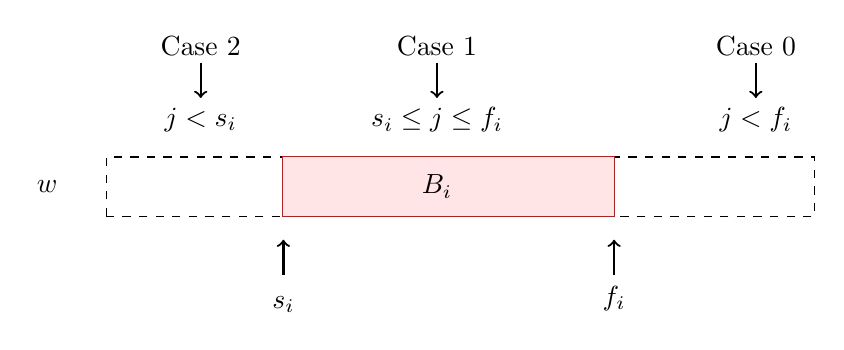
\begin{tikzpicture}[scale=1.5]
        % Main Rectangle w
        \draw[dashed] (0,0) rectangle (6,0.5);
        \node at (-0.5, 0.25) {\(w\)};

        % Smaller Rectangle 1 - Border color red
        \draw[draw=red, thick] (1.5,0) rectangle (4.3,0.5);
        
        \draw[->, thick] (1.5,-0.5) -- (1.5,-0.2);
        \node[align=center, below] at (1.5,-0.6) {\(s_{i}\)};
        \fill[red!10] (1.5,0) rectangle (4.3,0.5);
        \node at (2.8,0.25) {$B_{i}$};
        
        \draw[->, thick] (4.3,-0.5) -- (4.3,-0.2);
        
        \node at (4.3,-0.7) {$f_i$};
        
        
        \draw[->, thick] (5.5,1.3) -- (5.5,1);        
        \node[align=center, below] at (5.5,1) {\( j<f_i\)};
        \node[align=center, below] at (5.5,1.6) { \text{Case 0}};

        \draw[->, thick] (2.8,1.3) -- (2.8,1);        
        \node[align=center, below] at (2.8,1) {\( s_i \leq j \leq f_i\)};
        \node[align=center, below] at (2.8,1.6) {\text{Case 1}};

        \draw[->, thick] (0.8,1.3) -- (0.8,1);        
        \node[align=center, below] at (0.8,1) {\( j<s_i\)};
        \node[align=center, below] at (0.8,1.6) {\text{Case 2}};
        


    \end{tikzpicture}
    \caption{Compression for $w$ where $j$ is located.}
    \label{fig:case0}
\end{figure}


% So then, for case 0 $f_i<j$, it means that $s_i=s'_i$ and $f_i=f'_i$, LZ77 algorithm produces the exactly same result for $w[1,...,f_i]=w'[1,...,f_i]$, therefore. $B'_i$ is the only block that starts inside $B_i$, indeed, furthermore, $B_k=B'_k \forall k \leq i$.
% conclude that $f_i'\geq j$. When the case 1 holds, If $s_i\leq j\leq f_i$. We firstly have when $s_i=s'_i$, so that $B_k=B'_k \forall k \leq i-1$, this implies that $f_{i-1}=f'_{i-1}$. Hence $s_i=f_{i-1}+1 = f'_{i-1}+1 = s'_i$. We secondly have $f'_i\geq j$, so then, LZ77 compression only changes when a character is unknown for the string, thus, compression for $w'$ in the block $B'_i$ ends when $f_i=j$, moreover could be even greater, we never can finish before the index $j$ since compression up to $j$ is the same, so $|\mathcal{M}_i|= 1$ or $|\mathcal{M}_i|= 2$. Moreover, when $f'_{i+1}\geq f_i$, since $f_i\geq j$ we basically know that $f_i>f'_{i+1}$ but it does not matter how further $f'_{i+1}$ goes, because LZ77 compression guarantees that we can copy a substring that are previously encode. this automatically means that $|\mathcal{M}_i|= 2$ that is our important fact. On the other hand, analysis for case 2 relies when $j<s_i$ but based on LZ77 compression, when $j$ is placed before where the string for the block is copied over, it means that any place is located at compression for $w'$ adds at least 1 more block $B'_t$ that starts inside $B_k$ however since the condition holds we know that $f_i>f'_{i+1}$ therefore $|\mathcal{M}_i| \leq 2$.
% \end{proof}

% %%%%%%%%%%%%%%%%%%%%%%

% Let $t$ the maximum number of blocks after compressing $w'$ that \emph{Start Inside} $w$, since $w \sim w'$, then there is always a compression $(B'_1,...,B'_t)$ such as, WLOG $t'\geq t$ therefore, we defined $t'= \sum_{i=1}^{\infty}|\mathcal{M}_i|$, and $t= \sum_{i=1}^{\infty}|\mathcal{M}_i|$. These calculations are required for determine the quantity of blocks that \emph{Start Inside} either $B$ or $B'$ as a quantified property. Based on this reasoning and \defref{def:local_sensitivity} we introduce the difference to obtain Global Sensitivity, so then formally \claimref{claim:set:blocksm2:GS} as:
% %%%%%%%%%%%%%%%%%%%%%%%






% \lemblocknumupperbound

% \begin{proof}
%         If $i\in\B_2$ then either (1) $s_i\leq j\leq f_i$ or (2) $j-\ell_i < q_i \leq j$. When $j >f_i$, by LZ77 compression $B_i=B'_i$, thus $|\mathcal{M}_i|= 1$ and $i \in \mathcal{B_1}$.Hence, we have $s_i\leq j\leq f_i$ if $j\geq s_i$.
    
%     On the other hand, If $j<s_i$, then we want to show that $j-\ell_i<q_i\leq j$, i.e., $q_i\leq j < q_i+\ell_i$.
%     % \input{../Manuscript/figures/fig:claim9:case2}
%     Suppose for contradiction that $j\not\in[q_i,q_i+\ell_i-1]$.
%     Let $k$ be the smallest element in $\M_i$, i.e., $s_i\leq s_k'\leq f_i$ but $s_{k-1}'<s_i$.         
%     If $s_k'=f_i$, then if there is another $k'\in\M_i$ with $k'\neq k$, then by choice of $k$, we have $k<k'$ and therefore $s_{k'}'>f_k'>s_k'=f_i$. Hence, $|\M_i|= 1$ and $i\in\B_1$. Contradiction! It happens with any case for $j\not\in[q_i,q_i+\ell_i-1]$, since $i \in \B_2$. 
    
%     Now based on this, we are sure If $i_1,i_2\in\B_2$ then $(q_{i_1},\ell_{i_1})\neq(q_{i_2},\ell_{i_2})$. Since $i_1<i_2$ we then have $j<s_{i_1}<s_{i_2}$. Let $B_{i_1}=[q_{i_1},\ell_{i_1},c_{i_1}]$ and $B_{i_2}=[q_{i_2},\ell_{i_2},c_{i_2}]$ be  the blocks $B_{i_1}$ and $B_{i_2}$ of the LZ77 compression function $\compress:(\Sigma)^*\rightarrow(\Sigma')^*$ (Resp. w'). By intuition we know that there is no possibility to start in the same point for both Blocks $B_{i_1}$ and $B'_k$ after being read $j$ previously.
    

%     Finally Let $\B_2^\ell\coloneqq\{i\in\B_2:\ell_i=\ell\}$ and suppose that $s_{i^*}\leq j\leq f_{i^*}$ for some $i^*\in[t]$. Then $|\B_2^\ell|\leq\ell$ for all $\ell\neq \ell_{i^*}$, and $|\B_2^{\ell_{i^*}}|\leq\ell_{i^*}+1$. Furthermore, we observe that the constraint about length is: $\sum_{i\in\B_2} (\ell_i+1)\leq n,$ and $    \sum_\ell x_\ell'(\ell+1) < \sum_\ell x_\ell  (\ell+1) \leq n$. To find the threshold $z$, we observe that
% $\sum_{\ell=0}^z \ell(\ell+1) = \frac{1}{3}z(z+1)(z+2)\leq n,$
% which implies $z^3\leq 3n$ and $z\leq\sqrt[3]{3n}$. Setting this value of $z$, we have $t_2 \leq \frac{\sqrt[3]{9}}{2} n^{2/3} + \frac{\sqrt[3]{9}}{2} n^{1/3} + 1,$.
% \end{proof}

% The main result of this subsection is based on the analysis for upper bounding the global sensitivity, so then, in \secref{sec:upperbound} the goal is to provide the exact coefficient for the bound as is shown in the following theorem:




\section{Lower Bound for the Global Sensitivity of LZ77 Compression}\seclab{sec:lowerbound}

% =====

% \paragraph*{String Construction for the GS Lower Bound.}

% To prove the lower bound $\Omega(n^{2/3}\log^{1/3}n)$ for the global sensitivity of the LZ77 compression, we need to give example strings $w\sim w'$ of length $n$ that achieves $\left||\compress(w)|-|\compress(w')|\right|=\Omega(n^{2/3}\log^{1/3} n)$ (where $\compress$ denotes the LZ77 compression function) since this implies
% \begin{align*}
%     \mathtt{GS}_{\mathtt{Compress}} &= \max_{x \in \Sigma^n} \mathtt{LS}_{\mathtt{Compress}}(x)\\
%     &= \max_{x \in \Sigma^n}\max_{x' \in \Sigma^n:x\sim x'} \left| |\compress(x)| - |\compress(x')| \right|\\
%     &\geq \left||\compress(w)|-|\compress(w')|\right|\\
%     &=\Omega(n^{2/3}\log^{1/3} n).
% \end{align*}
% We give strings $w\sim w'$ that are carefully crafted such that $|w|=|w'|=\Theta(m^3\log m)$ for some integer $m>0$ and the number of type-2 blocks is $\Theta(m^2)$, which implies that $\GS_\compress=\Omega(m^2\log m) = \Omega(n^{2/3}\log^{1/3}n)$ where $n=\Theta(m^3\log m)$ denotes the length of strings. A core component of the string construction is to consider an \emph{injective encoding} of the number set $[m]$, which takes $\lceil\log m\rceil$ bits for each encoding, to ensure that each encoding is unique. This helps us count the number of type-2 blocks. However, having an injective encoding only does not fully resolve the issue 

% We overcome this bottleneck by \emph{repeating} each encoding twice.

% =====

In \secref{sec:upperbound}, we proved that the upper bound for the global sensitivity of the LZ77 compression algorithm $\compress$ is $O(n^{2/3}\log n)$ with window size $W=n$. One could ask if this is a tight bound, i.e., if we can prove the matching \emph{lower bound} for the global sensitivity of $\compress$ as well. This section proves the almost-matching lower bound up to a sub-logarithmic factor. In particular, we show that the global sensitivity of the LZ77 compression algorithm is $\Omega(n^{2/3}\log^{1/3} n)$. To prove the lower bound, we need to give example strings $w\sim w'$ of length $n$ that achieves $\left||\compress(w)|-|\compress(w')|\right|=\Omega(n^{2/3}\log^{1/3} n)$ since this implies $\GS_\compress=\max_{x \in \Sigma^n}\max_{x' \in \Sigma^n:x\sim x'} \left| |\compress(x)| - |\compress(x')| \right|\geq \left||\compress(w)|-|\compress(w')|\right|=\Omega(n^{2/3}\log^{1/3} n)$. 
% \begin{align*}
%     \mathtt{GS}_{\mathtt{Compress}} &= \max_{x \in \Sigma^n}\max_{x' \in \Sigma^n:x\sim x'} \left| |\compress(x)| - |\compress(x')| \right|\\
%     &\geq \left||\compress(w)|-|\compress(w')|\right|=\Omega(n^{2/3}\log^{1/3} n).
% \end{align*}
For the rest of \secref{sec:lowerbound}, we will give the construction of such example strings $w$ and $w'$.

\subsection{String Construction}

Consider an encoding function $\Enc:\mathbb{Z}\rightarrow\bin^*$ that maps integers to binary strings. Then for a positive integer $m\in\mathbb{Z}$, we have an injective encoding of the number set $\mathcal{S}\coloneqq\left\{0,1,\ldots, m\right\}$ using $\lceil\log m\rceil$ bits, i.e., $\Enc(i)\neq\Enc(j)$ if $i,j\in\mathcal{S}$ and $i\neq j$. For example, if $m=2^q-1$ for some positive integer $q$, we could encode the elements of $\S$ as follows: 
\[\Enc(0)=0^{\lceil\log m\rceil},\Enc(1)=0^{\lceil\log m\rceil-1}1,\Enc(2)=0^{\lceil\log m\rceil-2}10,\ldots,\Enc(m)=1^{\lceil\log m\rceil}.\] 
Now, consider a quinary alphabet $\Sigma=\{0,1,2,3,4\}$ and define a string
\[S_{\ell,u}\coloneqq\Enc(m-u+1)^2\circ\Enc(m-u+2)^2\circ\cdots\circ\Enc(m)^2\circ 2 \circ\Enc(m+1)^2\circ\cdots\circ\Enc(m-u+\ell)^2 \]
in $\Sigma^*$ for $2\leq\ell\leq m$ and $1\leq u\leq\ell-1$. 
Here, $(\cdot)^2$ denotes the concatenation of the string itself twice, i.e., $\Enc(\cdot)^2=\Enc(\cdot)\circ\Enc(\cdot)$. 
We define a procedure called $\QuinStr(m)$ which takes as input a positive integer $m\in\mathbb{Z}$ and outputs two quinary strings as follows.

\begin{tcolorbox}[breakable,enhanced,title={The Construction of Two Quinary Strings $\QuinStr(m)$.}]
    \begin{enumerate}
        \item The algorithm computes two quinary strings $S_w$ and $S_{w'}$ where
        \begin{align*}
            S_w &\coloneqq\Enc(1)^2\circ\cdots\circ\Enc(m)^2\circ 2 \circ\Enc(m+1)^2\circ\cdots\circ\Enc(2m)^2\circ 4,\text{ and}\\
            S_{w'} &\coloneqq\Enc(1)^2\circ\cdots\circ\Enc(m)^2\circ 3 \circ\Enc(m+1)^2\circ\cdots\circ\Enc(2m)^2\circ 4.
        \end{align*}
        \item Then it computes two quinary strings $w,w'$ defined as $w\coloneqq S_w\circ S$ and $w'\coloneqq S_{w'}\circ S$, where
        \[S = S_{2,1} \circ 4 \circ S_{3,2} \circ 4 \circ S_{3,1} \circ 4 \circ \ldots \circ S_{m,m-1} \circ 4 \circ \ldots \circ S_{m,1}\circ 4.\]
        \item Output $(w,w')$.
    \end{enumerate}
\end{tcolorbox}

\claimref{claim:length} tells us that the strings $w$ and $w'$ outputted by the procedure $\QuinStr(m)$ has equal length $\Theta(m^3\log m)$. Since the proof is elementary, we defer the proof of \claimref{claim:length} to \appref{app:missingprooflowerbound}.

\newcommand{\claimlength}{
Let $m\in\mathbb{N}$ and $(w,w')\gets\QuinStr(m)$. Then $|w|=|w'|=\Theta(m^3\log m)$. In particular, for $m\geq 4$, $\frac{2}{3}m^3\lceil\log m\rceil< |w|=|w'|< m^3\lceil\log m\rceil$.
}
\begin{claim}\claimlab{claim:length}
\claimlength
\end{claim}

\subsection{Analyzing the Sensitivity of $\QuinStr(m)$}

A central step in our sensitivity analysis for $\QuinStr(m)$ is precisely counting the type-2 blocks produced by the LZ77 compression scheme, as we observed in \secref{sec:upperbound}. \lemref{lem:gs} shows that for $(w,w')\gets\QuinStr(m)$, we have $|\B_2|=\frac{(m-1)m}{2}-(\lfloor\frac{m}{2}\rfloor-1)$. Intuitively, we first show that for $w=S_w\circ S$, there is no type-2 block for the blocks compressing $S_w$. Then the main insight is that we carefully crafted strings $w$ and $w'$ such that the marker symbol `4' becomes the endpoint for each block in $\compress(w)$ for the tail part $S$ of $w=S_w\circ S$. By repeating each encoding twice, we can ensure that most of the occurrences of $S_{\ell,u}\circ 4$ yield type-2 blocks, with an edge case (addressed in \claimref{claim:repeat}) that makes the block in $\B_1$ but this happens for only about $m/2$ blocks. Consequently, despite these few exceptions, the overall count of type-2 blocks remains quadratic in $m$.

\newcommand{\lemGS}{
Let $m\in\mathbb{N}$ and $(w,w')\gets\QuinStr(m)$ and let $\compress:\Sigma^*\rightarrow(\Sigma')^*$ be the LZ77 compression algorithm. Let $(B_1,\ldots,B_t)\gets\compress(w)$ and $(B'_1,\ldots,B'_{t'})\gets\compress(w')$. Then $|\B_0| = 0$ and $|\B_2| = \frac{(m-1)m}{2}-(\lfloor\frac{m}{2}\rfloor-1)$.
}
\begin{lemma}\lemlab{lem:gs}
    \lemGS
\end{lemma}

\begin{proof}
Recall that $w = S_w \circ S$ and $w' = S_{w'} \circ S$, where
\begin{itemize}
    \item $S_w =\Enc(1)^2\circ\cdots\circ\Enc(m)^2\circ 2 \circ\Enc(m+1)^2\circ\cdots\circ\Enc(2m)^2\circ 4$,
    \item $S_{w'}=\Enc(1)^2\circ\cdots\circ\Enc(m)^2\circ 3 \circ\Enc(m+1)^2\circ\cdots\circ\Enc(2m)^2\circ 4$, and
    \item $S=S_{2,1} \circ 4 \circ S_{3,2} \circ 4 \circ S_{3,1} \circ 4 \circ \ldots \circ S_{m,m-1} \circ 4 \circ \ldots \circ S_{m,1}\circ 4$, where
    \item $S_{\ell,u}\coloneqq\Enc(m-u+1)^2\circ\Enc(m-u+2)^2\circ\cdots\circ\Enc(m)^2\circ 2 \circ\Enc(m+1)^2\circ\cdots\circ\Enc(m-u+\ell)^2$ for $2\leq\ell\leq m$ and $1\leq u\leq \ell-1$.
\end{itemize}
We first observe that $w\sim w'$. Define $S_w^F\coloneqq \Enc(1)^2\circ\cdots\circ\Enc(m)^2\circ 2$ (resp. $S_{w'}^F\coloneqq \Enc(1)^2\circ\cdots\circ\Enc(m)^2\circ 3$) to be the first-half substring of $S_w$ (resp. of $S_{w'}$), and $S_w^L=S_{w'}^L\coloneqq \Enc(m+1)^2\circ\cdots\circ\Enc(2m)^2\circ 4$ to be the last-half substring of $S_w$ (or $S_{w'}$ since they are indeed identical). 
It is useful to define a notation $\str(B_k)$ for a block $B_k$, which denotes the substring of $w$ represented by the block $B_k$, i.e., for $B_k=[q_k,\ell_k,c_k]$, $\str(B_k)\coloneqq w[q_k,q_k+\ell_k-1]\circ c_k$. 

Let $B_{i_1}$ be the first block such that $S_w^F$ becomes a substring of $\str(B_1)\circ\str(B_2)\circ\ldots\circ\str(B_{i_1})$, and similarly, let $B'_{i'_1}$ be the first block such that $S_{w'}^F$ becomes a substring of $\str(B'_1)\circ\str(B'_2)\circ\ldots\circ\str(B'_{i'_1})$. Then we observe the following:
\begin{enumerate}
    \item $B_{i_1}=[q_{i_1},\ell_{i_1},2]$, i.e., $\str(B_{i_1})$ ends with $2$ (which is the last character in $S_w^F$), since $2$ never showed up before as all the encodings are binary strings, it has to be added to the dictionary as a new character,
    \item $B_i=B_i'$ for all $i\in[i_1-1]$, as we are compressing the identical strings until we see $2$ in $S_w^F$ (and $3$ in $S_{w'}^F$), and
    \item $i_1=i_1'$ and $B'_{i_1}=[q_{i_1},\ell_{i_1},3]$, since two strings $S_w^F$ and $S_{w'}^F$ are identical except for the very last character.\label{item:2}
\end{enumerate}

Now let $B_{i_2}$ be the first block such that $S_w^L$ becomes a substring of $\str(B_{i_1+1})\circ\str(B_{i_1+2})\circ\ldots\circ\str(B_{i_2})$, and similarly, let $B'_{i'_2}$ be the first block such that $S_{w'}^L$ becomes a substring of $\str(B'_{i_1+1})\circ\str(B'_{i_1+2})\circ\ldots\circ\str(B'_{i'_2})$. Then we observe the following:
\begin{enumerate}
\setcounter{enumi}{3}
    \item $i_2=i_2'$ and $B_i=B_i'$ for all $i\in[i_1+1,i_2]$, since $i_1=i_1'$ from observation \ref{item:2} and we have $S_w^L=S_{w'}^L$ while they do not contain $2$ or $3$, and
    \item $B_{i_2}=[q_{i_2},\ell_{i_2},4]$, since $4$ never showed up before in our compression.
\end{enumerate}

From the observations above, we have that $B_i\in\B_1$ for all $i\in[i_2]$. 
Now we are left with the blocks $(B_{i_2+1},\ldots,B_t)$ compressing the last part $S$ of $w$ and the blocks $(B'_{i_2+1},\ldots,B'_{t'})$ compressing the last part $S$ of $w'$. For the blocks $(B_{i_2+1},\ldots,B_t)$, we observe that each block ends at the next `$4$' because each $S_{\ell,u}$ (for $2\leq\ell\leq m$ and $1\leq u\leq \ell-1$) is contained in the former part of $w$ (which was $S_w$) but $4$ only shows up in $S_w$ followed by $\Enc(2m)^2$ while $S_{\ell,u}$ cannot contain $\Enc(2m)$. Hence, we observe the following:
\begin{enumerate}
\setcounter{enumi}{5}
    \item $\str(B_{i_2+1})=S_{2,1}\circ 4,\str(B_{i_2+2})=S_{3,2}\circ 4$,  and so on.
    \item In general, $\str\left(B_{i_2+\frac{(\ell-2)(\ell-1)}{2}+(\ell-t)}\right)=S_{\ell,u}\circ 4$, for $2\leq\ell\leq m$ and $1\leq u\leq \ell-1$. This indeed covers all the blocks from $B_{i_2+1},\ldots,B_t$ (See \claimref{claim:inj} and observation \ref{item:8}).
    \item Furthermore, we can observe that $t= i_2 + (1+2+\ldots+(m-1)) = i_2 + \frac{(m-1)m}{2}$.\label{item:8}
\end{enumerate}

\newcommand{\felluinjective}{
For any integer $m\geq 2$, the function $f(\ell,u)\coloneqq\frac{(\ell-2)(\ell-1)}{2}+(\ell-u)$ defined over integers $\ell$ and $u$ such that $2\leq \ell\leq m$ and $1\leq u\leq \ell-1$ is injective, and its range is $[\frac{(m-1)m}{2}]$.
}
\begin{claim}\claimlab{claim:inj}
\felluinjective
\end{claim}

The proof of \claimref{claim:inj} is elementary by induction on $m$, and hence, we defer the proof to \appref{app:missingprooflowerbound}. What we are interested in is whether each $B_i$, for $i_2+1\leq i\leq t$, belongs to $\B_0$, $\B_1$, or $\B_2$. In \claimref{claim:blocks}, we prove that the blocks are mostly in $\B_2$ and the rest of the blocks are in $\B_1$, meaning that $\B_0=\emptyset$. In particular, we prove that for $2\leq\ell\leq m$ and $1\leq u\leq\ell-1$, $B_{i_2+\frac{(\ell-2)(\ell-1)}{2}+(\ell-u)}\in\B_1$ if and only if all of these conditions hold: (1) $\ell>2$, (2) $\ell$ is even, and (3) $u=\ell/2$. 

\begin{claim}\claimlab{claim:blocks}
For $2\leq\ell\leq m$ and $1\leq u\leq \ell-1$, $B_{i_2+\frac{(\ell-2)(\ell-1)}{2}+(\ell-u)}\in\B_1$ if and only if $\ell>2, 2\mid\ell$, and $u=\ell/2$; otherwise $B_{i_2+\frac{(\ell-2)(\ell-1)}{2}+(\ell-u)}\in\B_2$.
%For $\ell'\in\left[\lfloor\frac{m}{2}\rfloor\right]$, $B_{i_2+(\ell'-1)(2\ell'-1)+\ell'}\in\B_1$ and 
\end{claim}

We will give the proof of \claimref{claim:blocks} below and finish the proof of \lemref{lem:gs} first for readability. By \claimref{claim:blocks}, since there are only $\lfloor\frac{m}{2}\rfloor-1$ of such pairs of $(\ell,u)$, we observe that $|\B_2|=\frac{(m-1)m}{2}-(\lfloor\frac{m}{2}\rfloor-1)$. Since we have that $B_i\in\B_1$ for all $i\in[i_2]$, we have $\B_0=\emptyset$ and therefore $|\B_0|=0$. This completes the proof of \lemref{lem:gs}.
\end{proof}

\begin{proofof}{\claimref{claim:blocks}}
Recall that $S=S_{2,1}\circ4\circ S_{3,2}\circ4\circ S_{3,1}\circ4\circ\ldots\circ S_{m,m-1}\circ4\circ\ldots\circ S_{m,1}\circ4$ and $\str(B_{i_2+1})=S_{2,1}\circ4$, $\str(B_{i_2+2})=S_{3,2}\circ4$, $\str(B_{i_2+3})=S_{3,1}\circ4,\ldots,\str(B_t)=S_{m,1}\circ4$. 
For each $S_{\ell,u}$, we observe that $S_{\ell,u}$ is \emph{not} a substring of $S_{w'}$. Hence, we see that each block $B_i$ (for $i_2+1\leq i\leq t$) is roughly split into two blocks for the blocks of $\compress(w')$ unless it could copy beyond the character $4$. To observe the cases when this happens,
for each $S_{\ell,u}$, it is helpful to define:
\begin{itemize}
    \item $S_{\ell,u}^F\coloneqq\Enc(m-u+1)^2$ denotes the very first encoding concatenation that shows in $S_{\ell,u}$, 
    \item $S_{\ell,u}^{F,(1/2)}\coloneqq\Enc(m-u+1)$ denotes the very first encoding in $S_{\ell,u}$ (i.e., half of $S_{\ell,u}^F$),
    \item $S_{\ell,u}^L\coloneqq\Enc(m-u+\ell)^2$ denotes the very last encoding concatenation that shows in $S_{\ell,u}$, and
    \item For $k>u$, $S_{\ell,u}^{(k)}\coloneqq\Enc(m-u+1)^2\circ\Enc(m-u+2)^2\circ\ldots\circ\Enc(m)^2\circ2\circ\Enc(m+1)^2\circ\ldots\circ\Enc(m-u+k)^2$ denotes the first $k$ encoding concatenations that shows in $S_{\ell,u}$.
\end{itemize}
Then we observe the following claims. Since proofs of \claimref{claim:notrepeat} and \claimref{claim:repeat} are elementary, we defer the proofs to \appref{app:missingprooflowerbound}.

\begin{claim}\claimlab{claim:notrepeat}
$S_{\ell,u}^L\circ4\circ S_{\ell,u-1}^F$ does not repeat for different $\ell$ and $u$ such that $3\leq\ell\leq m$ and $2\leq u\leq\ell-1$.
\end{claim}

\claimref{claim:notrepeat} tells us that, due to the injectivity of the encoding, any block in $\compress(w')$ containing a portion of $S_{\ell,u}^L$ along with the delimiter `4' must finish at $S_{\ell,u}^{F,(1/2)}$ in the worst case. In particular, note that $S_{\ell,u}^L=\Enc(m-u+\ell)^2=S_{\ell+1,u+1}^L$ for $3\leq \ell<m$ and $2\leq u<\ell-1$. Moreover, we have $S_{\ell,u-1}^{F,(1/2)}=\Enc(m-u+2)$ and $S_{\ell+1,u}^{F,(1/2)}=\Enc(m-u+1)$, which can agree on all but the final bit (e.g., $S_{\ell,u-1}^{F,(1/2)}=00\cdots00$ and $S_{\ell+1,u}^{F,(1/2)}=00\cdots01$). Without the repetition of each encoding, a block might incorporate nearly the entire $S_{\ell+1,u}^{F,(1/2)}$ except for the last bit. Consequently, by having this last bit as a new character, $S_{\ell,u-1}\circ4$ would be placed in $\B_1$. Repeating the encoding twice eliminates this possibility and we can ensure that the scenario described in \claimref{claim:repeat} is the only case where type-1 blocks would occur. Again, see \appref{app:missingprooflowerbound} for the proof of \claimref{claim:repeat}.


\begin{claim}\claimlab{claim:repeat}
For $2\leq\ell\leq\lfloor\frac{m}{2}\rfloor-1$, $S_{\ell,1}^L\circ4\circ S_{\ell+1,\ell}$ repeats at $S_{2\ell,\ell+1}^L\circ4\circ S_{2\ell,\ell}^{(\ell+1)}$.
\end{claim}

Let's go back to the proof of \claimref{claim:blocks}. By \claimref{claim:repeat}, we can see that the block of the form $B_{i_2+\frac{(2\ell-2)(2\ell-1)}{2}+(2\ell-\ell)}$ which satisfies
\[\str\left(B_{i_2+\frac{(2\ell-2)(2\ell-1)}{2}+(2\ell-\ell)}\right)=S_{2\ell,\ell}\circ4,\]
is in $\B_1$, and all of the other blocks beyond $B_{i_2}$ are in $\B_2$. This completes the proof of \claimref{claim:blocks}.
% We first observe the following.
% Now, let's analyze the blocks $(B'_{i_2+1},\ldots,B'_{i'_3})$. Consider $B'_{i_2+1}$ first as a warmup. Recall that $\str(B_{i_2+1})=S_{2,1}\circ 4$ because $S_{2,1}=\Enc(m)^2\circ 2\circ \Enc(m+1)^2$ was a substring of $S_w$, but this is \emph{not} the case for $w'$ since we replaced $2$ with $3$ in $S_{w'}$. This observation implies that $\str(B'_{i_2+1})=\Enc(m)^2\circ 2$ (which is the substring of $S_{2,1}$) since $\Enc(m)^2$ was contained in $S_{w'}$ and it is indeed the longest substring you could copy from the prior substring since $2$ never showed up in $w'$.
% Next, consider the next block $B'_{i_2+2}$. It is easy to see that $\str(B'_{i_2+2})=\Enc(m+1)^2\circ 4$ because $\Enc(m+1)^2$ is a substring of $S_{w'}$ and $4$ only showed up once in a prior substring, followed by $\Enc(2m)^2$ (in $S_{w'}\circ 4$). With a similar argument, we observe that $\str(B'_{i_2+3})=\Enc(m-1)^2\circ\Enc(m)^2\circ 2$ (which is a substring of $S_{3,2}$). Now for the block $B'_{i_2+4}$, one might think that $\str(B'_{i_2+4})=\Enc(m+1)^2\circ 4\circ c'_{i_2+4}$ where $c'_{i_2+4}$ is the first character in $\Enc(m)$ (since $S_{3,1}$ starts with $\Enc(m)^2$) since it seems to be the case that $\Enc(m+1)^2\circ 4$ is the longest substring of $S_{w'}\circ 4 \circ S_{2,1}\circ 4\circ \Enc(m-1)^2\circ\Enc(m)^2\circ 2$
\end{proofof}

Taken altogether, we can lower bound the global sensitivity of the LZ77 compression scheme as stated in \thmref{thm:lowerbound} below.

\begin{theorem}\thmlab{thm:lowerbound}
Let $\compress:\Sigma^*\rightarrow\Sigma'^*$ be the LZ77 compression function. Then $\mathtt{GS}_\compress\geq 4^{-1/3}\cdot n^{2/3}\log^{1/3}n=\Omega(n^{2/3}\log^{1/3}n)$. 
\end{theorem}

\begin{proof}
Let $(w,w')\gets\QuinStr(m)$ and let $|w|=|w'|=n$. By \claimref{claim:length}, we have $|w|=|w'|=\Theta(m^3\log m)$ and therefore $n=\Theta(m^3\log m)$. Furthermore, \claimref{claim:length} tells us that there exists some $\alpha$ with $\frac{2}{3}\leq\alpha\leq 1$ such that $n=\alpha m^3\log m$.  
Now let $(B_1,\ldots,B_t)\gets\compress(w)$ and $(B'_1,\ldots,B'_{t'})\gets\compress(w')$.
Recall that if we look at the proof of \claimref{claim:set:blocksm2:GS}, it tells us that $t'-t=|\B_2|-|\B_0|$. From \lemref{lem:gs}, we have $|\B_0|=0$ and $|\B_2|=\frac{(m-1)m}{2}-(\lfloor\frac{m}{2}\rfloor-1)$, which implies that $t'-t=\frac{(m-1)m}{2}-(\lfloor\frac{m}{2}\rfloor-1)$. We know $|\compress(w)|=t(2\lceil\log n\rceil+\lceil\log|\Sigma|\rceil)$ and $|\compress(w')|=t'(2\lceil\log n\rceil+\lceil\log|\Sigma|\rceil)$, we have
\begin{align*}
   \mathtt{GS}_{\mathtt{Compress}} & \leq  \left||\compress(w)|-|\compress(w')|\right|  
   = |t-t'|\left(2\lceil\log n\rceil+\lceil\log|\Sigma|\rceil\right) \\
    &= |t-t'|\left(2\left\lceil\log (\alpha m^3\log m)\right\rceil+\lceil\log|\Sigma|\rceil\right) 
    %\geq \left[\frac{(m-1)m}{2}-\left(\left\lfloor\frac{m}{2}\right\rfloor-1\right)\right]\cdot2\log(\alpha m^3\log m)\\
    \geq \frac{m^2}{4}\cdot 4\log m = m^2\log m \ .
\end{align*}
% \begin{align*} backup for full version
%     \left||\compress(w)|-|\compress(w')|\right| &= |t-t'|\left(2\lceil\log n\rceil+\lceil\log|\Sigma|\rceil\right) \\
%     &= |t-t'|\left(2\left\lceil\log (\alpha m^3\log m)\right\rceil+\lceil\log|\Sigma|\rceil\right)\\
%     &\geq \left[\frac{(m-1)m}{2}-\left(\left\lfloor\frac{m}{2}\right\rfloor-1\right)\right]\cdot2\log(\alpha m^3\log m)\\
%     &\geq \left(\frac{m^2}{2}-m\right)\cdot 4\log m\\
%     &\geq \frac{m^2}{4}\cdot 4\log m = m^2\log m,
% \end{align*}
%which implies that
%\begin{align*}
 %   \mathtt{GS}_{\mathtt{Compress}} &= \max_{x \in \Sigma^n}\max_{x' \in \Sigma^n:x\sim x'} \left| |\compress(x)| - |\compress(x')| \right|\\
 %   &\geq \left||\compress(w)|-|\compress(w')|\right|\\
  %  &= m^2\log m.
%\end{align*}
Furthermore, since we have $n=\alpha m^3\log m$ for some $\frac{2}{3}\leq\alpha\leq 1$, we observe that
\begin{align*}
    m^2\log m &= m^2\cdot\frac{n}{\alpha m^3}= \frac{n}{\alpha}\cdot\frac{1}{m} = \frac{n}{\alpha}\cdot\frac{\alpha^{1/3}\cdot\log^{1/3}m}{n^{1/3}}
    \geq \left(\frac{n}{\alpha}\right)^{2/3}\cdot 4^{-1/3}\cdot\log^{1/3}n \\
    &\geq 4^{-1/3}\cdot n^{2/3}\log^{1/3}n,
\end{align*}
% \begin{align*} backup for full version
%     m^2\log m &= m^2\cdot\frac{n}{\alpha m^3}\\
%     &= \frac{n}{\alpha}\cdot\frac{1}{m}\\
%     &= \frac{n}{\alpha}\cdot\frac{\alpha^{1/3}\cdot\log^{1/3}m}{n^{1/3}}\\
%     &= \left(\frac{n}{\alpha}\right)^{2/3}\cdot\log^{1/3}m\\
%     &\geq \left(\frac{n}{\alpha}\right)^{2/3}\cdot 4^{-1/3}\cdot\log^{1/3}n\\
%     &\geq 4^{-1/3}\cdot n^{2/3}\log^{1/3}n,
% \end{align*}
where the first inequality comes from the observation $\log n = \log\alpha + 3\log m + \log\log m\leq 4\log m$ and the second inequality comes from $(1/\alpha)\geq 1$. Hence,
\begin{align*}
    \mathtt{GS}_{\mathtt{Compress}} &\geq m^2\log m \geq 4^{-1/3}\cdot n^{2/3}\log^{1/3}n,
\end{align*}
% Since we know $\frac{2}{3}\cdot m^3\log m\leq n\leq m^3\log m$ from \claimref{claim:length}, we observe that 
% \begin{align*}
%     m^2\log m &= \frac{1}{m}\cdot m^3\log m\\
%     &\geq \frac{1}{m}\cdot n\\
%     &\geq \sqrt[3]{\frac{2}{3}}\cdot n^{-1/3}\cdot\left(\log^{1/3}m\right)\cdot n\\
%     &\geq \sqrt[3]{\frac{2}{3}}\cdot n^{-1/3}\cdot\left(\sqrt[3]{\frac{1}{6}}\cdot\log^{1/3}n\right)\cdot n\\
%     &= \sqrt[3]{\frac{1}{9}}\cdot n^{2/3}\log^{1/3}n,
% \end{align*}
% where the third inequality is achieved by the observation that $3\log m\geq \log n - \log\log m \geq \frac{\log n}{2}$, since $\log m\leq \sqrt{n}$.
% Hence,
% \begin{align*}
%     \mathtt{GS}_{\mathtt{Compress}} &\geq m^2\log m\\
%     &\geq \sqrt[3]{\frac{1}{9}}\cdot n^{2/3}\log^{1/3}n,
% \end{align*}
which completes the proof.
\end{proof}
\textit{Process:} We studies the influence of number of transformation operators ($N$) applied during the crossover for each candidate. We investigated the effectiveness and efficiency of Codeimprove under different settings, i.e., $N$ = \{2, 5, 10, 15\}. We applied variable renaming and one random transformation operator from Table~\ref{table:transformations} for $N=2$, operators 1-5 for $N$=5, operator 1-10 for $N$=10, and operators 1-15 for $N$=15. 


\textit{Results: }Table~\ref{Tab:sensitivity} show the results of CodeImprove under the hyper-parameter settings of $N$ in terms
of CSR, MCR, and RI. \textcolor{blue}{We observed that as N increases, more mispredicted inputs can be corrected, resulting in a larger RI.}
%We found with the setting of $N$ increasing, the more mispredicted inputs can be corrected resulting to a larger RI. 
Meanwhile more correctly predicted inputs are identified as mispredicted ones due to more transformations leading to slightly higher MCR. When $N$ = 5 for CodeBERT on vulnerability detection task, \textcolor{blue}{CodeImprove} achieved a higher CSR (i.e., 40.3\%) than $N$=10 (i.e., CSR of 38.7\%), however the RI \textcolor{blue}{was lower than} $N$ =10 due to higher MCR value. Therefore, it is necessary to maintain the balance between CSR and MCR during the transformation. Moreover, CodeImprove has achieved greater performance on all cases for $N$, \textcolor{blue}{indicating its practical applicability}. 


\begin{tcolorbox}[title=\textbf{RQ4} - How sensitive is CodeImprove’s performance under different experimental setups?, left=2pt, right=2pt,top=2pt,bottom=2pt]
CodeImprove is effective when different number of transformation operators are applied during the crossover (i.e., RI shows 48.4\% - 51.28\% for vulnerability detection and 26.1\%-32.8\% for defect detection tasks).
\end{tcolorbox}
%\vspace{-3mm}






%%%ISSTA\subsection{RQ3: Impact on Layer Selection for Out-of-Scope Data Detection}

 %Our goal is to analyze how out-of-scope data detection affects on growing layers. Therefore, we randomly selected four sub-models from our study to compute the number of out-of-scope data detected by our validity score. We selected sub-models of layers consisting of one, four, seven, and twelve. Note that for all models in the subject, the maximum number of layers is 12. Table~\ref{Tab:rq3} shows the statistics of the AUC comparison of validity score with different numbers of sub-models. Table~\ref{Tab:rq3}, column 2 shows the selected layer ids of each sub model. 

 %%%ISSTA \textit{Process} Our goal is to analyze how out-of-scope data detection affects on growing layers. We randomly selected sub-models consisting of one, four, seven, and twelve layers. Table~\ref{Tab:rq3} presents the statistics of the AUC comparison and Column 2 of Table~\ref{Tab:rq3} shows the selected layer ids of each sub-model. Note that for all models in the subject, the maximum number of layers is 12.
 
 
 %Table~\ref{Tab:rq3} presents the statistics of the AUC comparison of the validity score with different numbers of sub-models, which were randomly selected from the generated sub-models. The sub-models consist of one, four, seven, and twelve layers. Column 2 of Table~\ref{Tab:rq3} shows the selected layer ids of each sub-model. Note that for all models in the subject, the maximum number of layers is 12.



%From Table~\ref{Tab:rq3}, we observe that: (1) highest AUC scores are obtained in sub-models with less number of layers (i.e., sub-model-1 except for RoBERTa on vulnerability detection); (2) adding more layers will show a decreasing pattern of AUC scores (e.g. 0.798 vs 0.874 for vulnerability detection on BERT with sub-model-12 vs sub-model-1); (3) RoBERTa model on vulnerability detection shows lowest AUC score for sub-model 1,4,and 7 respectively; (4) defect prediction task with 1 sub-model achieved the highest AUC scores; and (5) although all sub-model performs satisfactorily, we can conclude that adding layers can affect the final model prediction. Therefore, different layers affect in overall model performance. 

%%%ISSTA From Table~\ref{Tab:rq3}, we observe that: (1) sub-models with fewer layers (i.e., sub-model-1 except for RoBERTa on vulnerability detection) achieved the highest AUC scores; (2) adding more layers showed a decreasing pattern of AUC scores (e.g. 0.798 vs 0.874 for vulnerability detection on GraphCodebERT with sub-model-12 vs sub-model-1); (3) RoBERTa model on vulnerability detection shows the lowest AUC score for sub-model-1, sub-model-4, and sub-model-7 respectively; (4) the defect prediction task with one sub-model achieved the highest AUC scores (i.e., 0.928-0.936); and (5) although all sub-models performed satisfactorily, we can conclude that adding layers can affect the final model prediction. Therefore, different layers have an impact on the overall model performance.

%%%issta\begin{tcolorbox}[title=\textbf{RQ3} - Does the choice of layers for selection have an impact on out-of-scope data detection?, left=2pt, right=2pt,top=2pt,bottom=2pt] Layer selection for detecting out-of-scope data is important for its best effectiveness (Table~\ref{Tab:rq3}). 
%%%\end{tcolorbox}


 





\section{Case Study on SafeSPLE}
We now demonstrate via a case study one way to implement a SafeSPL and parameterized safety cases.  The first part of our process is a hazard analysis. We then build a feature model. The features are then used to parameterize our safety case. Lastly, we can generate safety-case instances as requested for any of the concrete combinations of features.  

\subsection{Hazard Analysis}
To begin the SafeSPLE process for a UAS flight, we analyze the hazards of that flight, which is an important first step before creating a safety case \cite{Knig12}. A hazard is a state or event that can potentially result in an accident \cite{ericson2015hazard}. In this work, we do not describe this part of the process in depth but rather list a few of the key hazards we identified. We utilized several sources to create our list of hazards. First, we referenced several papers describing hazard analysis or safety cases for sUAS flights \cite{denpai2016, clodenpai2017, sora}. Next, we discussed sUAS hazards with colleagues and experts who have studied sUAS and flown them. This investigation gave us an extensive list of hazards, which was too long and broad to include in this paper. We narrowed down this extensive list to focus on the following hazards. 

\begin{itemize}
    \item Too much precipitation
    \item Insufficient visibility
    \item Temperatures outside the operating specifications of the sUAS
    \item Wind gusts outside the operating specifications of the sUAS
    \item Insufficient battery for the mission
\end{itemize}

The hazards above are not intended to be fully described or defined, and we do not include prevention or recovery controls or escalation factors for any of these hazards (see \cite{denpai2016} for a more in-depth discussion of hazard analysis). The ultimate consequences of each of the above hazards are generally either loss of separation from the ground or loss of separation from other air traffic. Either of these consequences could lead to the destruction of property, injury, or death. A complete risk analysis of these consequences is likewise beyond the scope of this paper. We illustrate our family-based approach below using a subset of the identified hazards in order to show how the parameterized safety case addresses the hazards for different sUAS.       

\subsection{Feature Model}

\begin{figure}[ht]
    \centering
    \includegraphics[width=.8\textwidth]{Figures/safety-case-blow-up.pdf}
    \caption{Two parts of the feature model that we focus on for this case study.}
    \label{fig:feature_model_focus}
\end{figure}

The next step in the SafeSPLE process is to create a partial feature model that could apply to a wide variety of sUAS models and missions in controlled airspace as described in Section \ref{sec:SafeSPLE} and Figure \ref{fig:featuremodel}. Since this feature model includes information about the pilot, airspace, mission, vehicle, and weather (among other things), it allows for a wide variety of different types of parameters to be used in our parameterized safety case. In figure \ref{fig:feature_model_focus} we show the two parts of the feature model that are the focus of our safety cases here - the pilot and the weather. These parameterized safety cases are described in the next section. 


\subsection{Parameterized Safety Case}

\begin{figure}[ht]
    \centering
    \includegraphics[width=.7\textwidth]{Figures/pilot_only.pdf}
    \caption{Pilot Safety Case: A safety case based only on whether the pilot is certified and has sufficient experience.}
    \label{fig:pilot_only}
\end{figure}

The next step in our case study (based on SafeSPLE) is to create two illustrative parameterized safety cases for our controlled airspace. The first safety case, seen in Figure \ref{fig:pilot_only}, is based solely on the pilot. It checks whether the pilot is certified and has sufficient flight hours. We assume that in non-commercial airspaces, flight regulations would trust a certified pilot with sufficient reputation (i.e., no significant history of problems) to perform safety checks consistent with the lower-level details of our safety cases. In other words, the pilot is in charge of ensuring a safe flight in whatever airspace they are in. Regulators often do not exclude pilots legally allowed to be in the airspace unless there is some serious prior issue \cite{FAA_TRUST, FAA_part107}. So it is our belief that any UAS Traffic Management system will likely allow certified pilots to enter the airspace unless it has some reason not to.

As shown in Figure \ref{fig:pilot_only}, our safety case checks to see if the pilot is certified to fly their sUAS, here represented using the FAA's Part 107 certification \cite{FAA_part107}. We also check to see if the pilot has sufficient flight hours to be competent to complete this flight, which is something that our managed airspace should know.  In the future, this flight-hours check might be replaced or augmented with different checks, such as the pilot's score on a competency-reputation metric, future certifications, or temporary notices to pilots that the FAA might put out. If evidence of these checks confirms that the pilot is certified and has sufficient experience to enter the controlled airspace, the associated strategy node (S1) in the safety case is satisfied.

\begin{figure}[ht]
    \centering
    \includegraphics[width=\columnwidth]{Figures/wind_only.pdf}
    \caption{Wind Safety Case: A parameterized safety case based only on the weather and the drone's capabilities. This safety case creates the instances seen in Figures \ref{fig:instance_1} and \ref{fig:instance_2}.}
    \label{fig:wind_only}
\end{figure}

Our second safety case is relevant when the pilot lacks the evidence required to satisfy our initial safety case above. There needs to be an opportunity for newer pilots to learn and fly if such flights can be done safely. Thus, our second safety case focuses on giving such pilots the information that they will need in order to complete a safe flight. This second safety case (Figure \ref{fig:wind_only}) focuses on the weather because poor weather is a common reason for a pilot to decide that a flight will not be safe or for in-flight failures \cite{weather_hazards_for_UAV}. The weather portion of the feature model also has several parameters that can map to portions of our safety case. This sort of weather-focused safety case would normally involve far more attributes than we show in Figure \ref{fig:wind_only}, but we focus only on the weather and a small amount of information (evidence) about the battery here.

In the wind safety case from Figure \ref{fig:wind_only}, we constructed a general safety case that involves a number of parameters that are found in our feature model. These parameters are indicated using square brackets, such as [Precipitation] and [UASAllowedPrecipitation]. The data types of each parameter are left intentionally vague, as there are a number of ways for these parameters to be stored. We assume that information about each [Vehicle] is publicly available and that published sUAS specifications can be converted into the same data format and type that the feature model and safety case parameters have. If a [Vehicle] does not contain information in its specifications for certain parameters, then there is an option to assume some default values that could apply to almost all drones. 

For instance, most sUAS specifications will include information about the maximum allowed wind speed within which the manufacturer states the sUAS can operate. Likewise, most sUAS specifications include both maximum and minimum allowed temperatures in which to operate (often from -10 \textcelsius \;or 0 \textcelsius \;up to 40 \textcelsius) \cite{DEERCD20, DJI_MiniPro_4_Specs}. Fewer sUAS specifications contain specific information about visibility requirements since those depend on the type of mission being flown, especially whether it needs to be flown in a visual line of sight (VLOS) or beyond a visual line of sight (BVLOS). If the pilot does not provide visibility requirement information, we thus assume that the flight must take place VLOS and proceed accordingly. Similarly, if no information is provided about an sUAS's ability to fly in various forms of precipitation, we assume that the sUAS can only operate with no precipitation. 

Note that in the wind safety case (Figure \ref{fig:wind_only}), many of the goals share a similar structure. For instance, "The forecast precipitation is within acceptable level..." and "The forecast visibility is within acceptable levels...". The repetition of these elements is intentional and allows for greater ease of human understanding of the safety case, as well as for simpler extension of the safety case when we add additional hazards we need to mitigate. 

Some of the values of the parameters in the safety case may not be available at the time of a flight request. For instance, if a pilot is applying to complete a flight several weeks or months in the future, the forecast weather conditions will be unreliable. In such a case, the safety case might not contain concrete values until closer to the flight. The pilot could still access the parameterized safety case in order to study the safety requirements for the flight. As the time of the flight approaches, a more fully instantiated safety case could be sent to the pilot. 

The information for instantiating these parameterized safety cases will need to be pulled from a variety of sources, such as publicly available weather data and manufacturers' specifications for commercially available sUAS. However, some of the parameters' information will need to come from the pilot, including their certification status, the sUAS model they will fly, their flight plan, and any additional sUAS capabilities they have added (such as detect-and-avoid systems). 
In the event that the sUAS being flown was completely home-built, there may be no public documentation of its abilities, and all of its specifications will need to be provided (or inferred) by the pilot. 
Therefore, some of the individual safety cases will necessarily contain a fair amount of uncertainty while still serving as a guideline for the pilot. 


\subsection{Instances}
As a final step in our SafeSPLE process, we demonstrate how to create instances of our parameterized safety case. This process involves obtaining the information required for all parameters and checking if all the solution nodes of the safety case remain true. In all of the safety case diagrams in Figures \ref{fig:pilot_only}, \ref{fig:wind_only}, \ref{fig:instance_1}, \ref{fig:instance_2}, these solution nodes are the bottom nodes labeled E1-E6, and have propagated from the context. If any solution node becomes false, then we can say that the pilot should either reconsider the flight, or should implement further mitigations to reduce the risk from the relevant hazard. For instance, if the safety case shows that the current wind gusts are too high, the pilot might delay the flight until the wind calms, or the pilot might decide to make the flight with a larger and more capable UAS (if available).

\begin{figure}[ht]
    \centering
    \includegraphics[width=.95\textwidth]{Figures/Instance_1.pdf}
    \caption{Safety Case Instance 1: An instance of the wind safety case (Figure \ref{fig:wind_only}) based on a mission with a DJI Mini 4 Pro drone.}
    \label{fig:instance_1}
\end{figure}

The first instance of our parameterized safety case is shown in Figure \ref{fig:instance_1}. This mission will be performed by a DJI Mini 4 Pro, a widely available drone that currently sells for just over \$1000, depending on accessories. The Mini 4 Pro is fully charged, and the mission, as planned, should take 16 minutes, flown entirely within VLOS of the pilot. This information about battery charge and the mission plan is provided by the pilot. The wind is gusting up to 6 meters/sec, with temperatures in the mid 20s \textcelsius, unlimited visibility, and no precipitation. This weather information is provided to the safety case by a commercial or governmental weather service. 

Once we obtain the information about the make and model of the drone, we can look up the DJI's published specifications. According to DJI \cite{DJI_MiniPro_4_Specs}, the Mini 4 Pro is able to fly in wind speeds up to 10 m/s, and with a fully charged battery can fly up to 34 minutes. The Mini 4 Pro can operate in temperatures between -10 \textcelsius \;and 40 \textcelsius. Using all this information, we can instantiate the safety case seen in Figure \ref{fig:instance_1}. Note that every solution node 
(labeled E1-E6) is satisfied by the above information. There is no precipitation; visibility is unlimited; the temperatures are not too hot or cold; the wind gusts are below the max allowed for the drone; and the battery reserves are more than twice as much as needed. So in this instance of the safety case the the top-level goal is satisfied. 

\begin{figure}[ht]
    \centering
    \includegraphics[width=.95\textwidth]{Figures/Instance_2.pdf}
    \caption{Safety Case Instance 2: An instance of the wind safety case (Figure \ref{fig:wind_only}) based on a mission with a DEERC D20 drone. Note that this instance fails to fulfill our safety requirements at node E4 (marked in darker red).}
    \label{fig:instance_2}
\end{figure}
%Nice examples!

In Figure \ref{fig:instance_2} we can see a second instance of our safety case. This mission will be performed by a DEERC D20 drone, another widely available drone that currently sells for around \$50. The D20 is also fully charged, and the planned mission will only take 5 minutes of flying, entirely within VLOS. The wind is gusting up to 8 m/s, with temperatures in the mid-30s \textcelsius, 3 km visibility, and no precipitation.

According to the DEERC documentation \cite{DEERCD20}, the D20 drone is capable of about 10 minutes of flight time in temperatures between 0 \textcelsius \ and 40 \textcelsius. However, the D20 documentation does not specify the maximum speed of the winds that the drone is capable of flying in. Instead, the documentation reads, "DO NOT use this drone in adverse weather conditions such as rain, snow, fog, and wind." Therefore the safety case takes a conservative approach and assigns a default value of 3 m/s to the variable [MaxAllowedWindSpd] (3 m/s is slightly less than 7 mph). This default value could, of course, be set to 0 m/s, although this seems unrealistic for most outdoor flying. Other default values might be justified.

Plugging in all of these values, we see that while most solution nodes are satisfied, the current wind conditions (gusts up to 8 m/s) do not allow for a safe flight with the D20 (default max wind speed of 3 m/s). In Figure \ref{fig:instance_2}, this is shown at solution node E4, which is colored a darker red than the other solution nodes. The safety case is designed to serve as input to the UTM on-entry decision. At this point there are two main options for how the UAS Traffic Manager could behave. The UTM could refuse entry to this pilot until the wind speed is lower, or the UTM could send the safety case to the pilot with the recommendation that the pilot make modifications to the flight plan while leaving the ultimate flight decision up to the pilot.

Creating instances of safety cases with SafeSPL should be quick and relatively straightforward, if the information it needs is available. If information on the drone's capabilities is lacking, default values can still allow the safety case to create a reasonable instance. If information about the weather is unknown, then those portions of the safety case can be left uninstantiated until more detailed information becomes available. At the very least, we can generate a partially instantiated safety case so the pilot can see the areas where information is lacking or is based on default values. This information could allow the pilot to focus on mitigation measures in those areas if needed. 

\subsection{Connecting to Safe Entry}
\label{sec:safe_entry}

The parameterized safety cases created by SafeSPLE and described above could play an important role in a to-be-developed UTM system. When a pilot requests permission to fly in the airspace controlled by the UTM, the information needed to instantiate the safety case is either submitted by the pilot or looked up by the UTM system. Once a safety case has been created for that flight, there are at least two options for what the UTM system might do with it. 

\begin{enumerate}
    \item Closed Access: The UTM system accepts or denies requests based on whether each generated safety case "passes" or "fails". In other words, if the safety case goals are not satisfied, the UTM system  denies the flight. 
    \item Open Access: The UTM system accepts or denies the flight based solely on whether the pilot is certified or trusted. The safety case then becomes a guideline that can be provided to the pilot as something of a checklist to encourage a safer flight.
\end{enumerate}

Which action the UTM should take is an ongoing discussion with no immediate correct answer.
Currently the regulations in the US appear to generally favor approach (2), the open-access model. Regardless of which approach is taken for a specific controlled airspace, we believe the use of SafeSPLE will generate valuable on-the-fly information.  This information may offer an effective and useful checklist for decision-making. 


%We measure the effectiveness of applying semantic preserving program transformations to adapt out-of-scope inputs to become in-scope inputs. We compute IDP for each subject model with CodeImprove and CodeImprove-random. In particular, CodeImprove-random applies 10 randomly selected program transformation rules for out-of-scope inputs. We set the random transformation number to 10 in order to maintain the diversity of the transformed programs. Table~\ref{Tab:rq4} shows the statistics of IDP comparison for CodeImprove and CodeImprove-Random. 

%From Table~\ref{Tab:rq4}, we observe that: (1) CodeImprove performed better in terms of IDP in all subject matter compared to CodeImprove-random, suggesting that CodeImprove is more effective in converting an out-of-scope input to an in-scope input; (2) CodeBERT models on both SE tasks obtained the highest IDP values (i.e., 16.77 and 12.04); (3) CodeImprove-random showed similar IDP value for RoBERTa model on defect prediction task compared to CodeImprove (8.35 vs 10.06); and (4) overall, adapting an out-of-scope input to an in-scope input is satisfactory and promising by utilizing CodeImprove. 

% \begin{figure}
%      \centering
%      \begin{subfigure}[b]{0.5\columnwidth}
%      \begin{minted}{C}
% for(iter = m.begin(); iter != m.end(); iter++){
% //
% }
% \end{minted}
% \caption{Defining \textit{for-loops} with before C++14}
% \label{fig:y equals x}
% \end{subfigure}
% \hfill
% \begin{subfigure}[b]{0.5\linewidth}
% \begin{minted}{C}
% for(auto:iter m){
% //
% }      
% \end{minted}
% \caption{Defining \textit{for-loops} with C++14}
% \label{fig:three sin x}
% \end{subfigure}
% \caption{Difference in the Definition of for-loops before and after C++14}
% \label{fig:forloops}
% \end{figure}
%-------------------------------------
% \noindent\begin{minipage}{.48\textwidth}
% \begin{minted}{C}
% static int null_filter_samples(AVFilterLink *link, 
% AVFilterBufferRef *samplesref){   
% return 0;}

% \end{minted}
% \end{minipage}\hfill
% \begin{minipage}{.45\textwidth}
% \begin{lstlisting}[caption= Transformed in-scope Input,frame=tlrb]{Name}
% void code()
% {

% }
% \end{lstlisting}
% \end{minipage}


% \noindent\begin{minipage}{.48\textwidth}
% \begin{lstlisting}[caption= An out-of-scope Input,frame=tlrb]{Name}
% void code()
% {

% }
% \end{lstlisting}
% \end{minipage}\hfill
% \begin{minipage}{.45\textwidth}
% \begin{lstlisting}[caption= Transformed in-scope Input,frame=tlrb]{Name}
% void code()
% {

% }
% \end{lstlisting}
% \end{minipage}






%\begin{table}[htb!]
\caption{Effectiveness of Program Transformation on Incorrectly Predicted Inputs}
\label{Tab:misclassified}
\renewcommand{\arraystretch}{1.12}
\resizebox{0.95\columnwidth}{!}{
\begin{tabular}{|c|c|c|c|c|c|c|c|c|}
\hline
 \multirow{2}{*}{\textbf{Model}} &\multicolumn{4}{c|}{\textbf{Vulnerability Detection}} & \multicolumn{4}{c|}{\textbf{Defect Prediction}}\\ \cline{2-9}
      &Accuracy & Precision & Recall & F1-Score & Accuracy & Precision & Recall & F1-Score \\ \hline

  

   

     CodeBERT & %69.48 
    71.23  & 71.45  & 62.24 & 66.53 & 85.42 & 85.17 & 85.42 & 85.06 \\\hline

    RoBERTa & 64.09 & 60.65 & 62.15  & 61.39 & 83.78& 83.83& 83.78 & 83.22  \\\hline

    BERT & 63.50 & 59.96 & 61.83 & 60.88& 79.81& 79.91 & 79.81 & 79.45 \\\hline
  
  
\end{tabular}
}
\end{table}

%In addition to computing the IDP values, we sampled the incorrectly predicted inputs in Table~\ref{Tab:stts} to apply our program transformation. The results are shown in the Table~\ref{Tab:misclassified}. We find that CodeImprove is capable of improving the model performance of each subject in terms of accuracy, precision, recall, and F1-score compared to the performance of original set up (e.g: an increase of accuracy: 2.53\% - 8.49\%, precision: 2.29\%-9.15\%, recall: 1.04\%-14.43\%, and F1-score: 2.03\%-12.42\%). 


\begin{tcolorbox}[title=\textbf{RQ5} - Does program transformations of
CodeImprove preserve semantics?, left=2pt, right=2pt,top=2pt,bottom=2pt]
CodeImprove can generate semantic preserving program transformations. 
\end{tcolorbox}




\subsection{RQ6: Overhead of CodeImprove}

%\textcolor{red}{organize this section to show online offline stage.}
\textcolor{blue}{\textit{Process: } To apply CodeImprove in real-time, we compute the overhead of applying transformations for an input. We calculate the TPS, which measures the number of transformations applied per second by CodeImprove. This metric is averaged across all $N$ variants of CodeImprove studied under RQ4. Additionally, we evaluate both offline and online overhead. The offline stage involves the sub-model training, while the online stage measures the time required to adapt an input with CodeImprove. Table~\ref{Tab:rq5} shows the statistics of TPS, and Figure~\ref{fig:combined_figures} shows the time overhead of CodeImprove.   }


%\textit{Process: }  In order to apply CodeImprove in real-time, we compute the overhead of applying transformation for an input. We compute the TPS, which measures the number of transformations applied per second by CodeImprove.  This is the average of all $N$ variants of CodeImprove studied under RQ4. Table~\ref{Tab:rq5} shows the statistics of overhead for adapting an out-of-scope input by CodeImprove. %Note that we applied CodeImprove on all samples in Table~\ref{newstats}. 

\begin{table}[!t]
    \centering
    % \scriptsize
    \tiny
    \tabcolsep=15pt
    % \footnotesize
    % \renewcommand{\arraystretch}{1.2} 
    \caption{\revise{Performance on adaptive attacks.}}
    \vspace{-1mm}
    \label{tab:rq5}
    \begin{tabular}{ccccc}
        \toprule
        
        \multirow{2}{*}{Task Dataset/Attack} & \multicolumn{2}{c}{MixUp} & \multicolumn{2}{c}{\revise{BadCode-PPL (perplexity)}} \\

        \cmidrule(lr){2-3} \cmidrule(lr){4-5}
        
        & FPR & Recall & \revise{FPR} & \revise{Recall} \\
        
        \midrule

        Defect Detection & 9.15\% & 95.67\% & \revise{12.23\%} & \revise{96.55\%} \\

        Clone Detection & 5.32\% & 100\% & \revise{7.45\%} & \revise{93.64\%} \\

        Code Search & 5.99\% & 94.06\% & \revise{6.32\%} & \revise{94.31\%} \\

        Code Repair & 1.12\% & 96.19\% & \revise{2.17\%} & \revise{95.23\%} \\

        \midrule
        
        Average & 5.40\% & 96.48\% & \revise{7.05\%} & \revise{94.93\%} \\
        
        \bottomrule
        
    \end{tabular}
    \vspace{-4mm}
\end{table}
\vspace{-1em}
\textcolor{blue}{Based on  Table~\ref{Tab:rq5}, CodeImprove is capable of applying transformations at a rate of 1.2 TPS to 2.04 TPS for each SE task across all code models. Figure~\ref{fig:figure2} confirms that CodeImprove takes approximately 49.92s to 59.4s to adapt an input across all models. We plan to further minimize the transformation times in future work.  Moreover, CodeImprove is more efficient and offers a practical, scalable solution to enhance model performance without the significant cost and time investment required by traditional methods such as retraining and replacement.}
\vspace{-1em}
\begin{figure}[H]
    \centering
    \begin{subfigure}[b]{0.49\columnwidth}
        \centering
        \includegraphics[width=\columnwidth]{tex/images/offline_stage_time_comparison_similar_bold.pdf}
        \caption{\textcolor{blue}{Offline time overhead (in second)}}
        \label{fig:figure1}
    \end{subfigure}
    \hfill
    \begin{subfigure}[b]{0.49\columnwidth}
        \centering
        \includegraphics[width=\columnwidth]{tex/images/online_stage_time_comparison_similar_bold.pdf}
        \caption{\textcolor{blue}{Online time overhead (in seconds)}}
        \label{fig:figure2}
    \end{subfigure}
    \caption{\textcolor{blue}{Time Overhead of CodeImprove}}
    \label{fig:combined_figures}
\end{figure}
\vspace{-1em}
\textcolor{blue}{It is important to note that the sub-model training procedure is treated as an offline stage, minimizing its impact on overall performance. Figure~\ref{fig:figure1} shows that training a sub-model takes around 900s to 940s for the vulnerability detection  and 1200s to 1250s for the defect prediction across all models on a machine with an NVIDIA GeForce GTX 1080 GPU. This process only needs to be done once and incurs significantly lower costs compared to regular retraining or fine-tuning.}


%It is important to note that the sub-model training procedure is treated as an offline stage, minimizing its impact on overall performance. Training sub-models with 12 layers takes approximately three to five hours (i.e., 15 to 25 minutes per sub-model) on a machine with an NVIDIA GeForce GTX 1080 GPU and only needs to be done once. This process incurs significantly lower costs compared to regular retraining or fine-tuning.

%%%From the Table~\ref{Tab:rq5}, an average CodeImprove takes around one minute to adapt an input (1.2 TPS to 2.04 TPS), confirming that CodeImprove is capable of adapting inputs in practical use. \textcolor{blue}{We plan to further minimize the transformation times in future work. Moreover, CodeImprove is more efficient and offers a practical, scalable solution to enhance model performance without the significant cost and time investment required by traditional methods such as retraining and replacement. }

% \begin{figure}[H]
%     \centering
%     \begin{minipage}[b]{0.49\columnwidth}
%         \centering
%         \includegraphics[width=\columnwidth]{tex/images/offline_stage_time_comparison_similar_bold.pdf}
%         \caption{(a) Offline stage time comparison}
%         \label{fig:figure1}
%     \end{minipage}
%     \hfill
%     \begin{minipage}[b]{0.49\columnwidth}
%         \centering
%         \includegraphics[width=\columnwidth]{tex/images/online_stage_time_comparison_similar_bold.pdf}
%         \caption{(b) Online stage time comparison}
%         \label{fig:figure2}
%     \end{minipage}
%     \caption{Combined caption for both figures}
%     \label{fig:combined_figures}
% \end{figure}








%Therefore, our approach is more feasible and efficient, avoiding extensive overhead of retraining or replacement. We plan to further minimize these transformation times as a future work. By focusing on input adaptation, we offer a practical and scalable solution to enhance model performance without the significant costs and time investments of traditional methods. }



%our approach of adapting inputs is more feasible and efficient, avoiding the extensive overhead of retraining or replacement. We are also working on further minimizing these transformation times. By focusing on input adaptation, we offer a practical and scalable solution to enhance model performance without the significant costs and time investments of traditional methods.





%%Note that the sub-model training procedure is treated as an offline stage, minimizing the impact on overall performance. Each sub-model inherits the weights of the original model up to a certain layer, with minimal training on dense and dropout layers to introduce variability. Training sub-models with 12 layers takes approximately three to five hours (i.e., 15 to 25 minutes for each sub-model) on a machine with an NVIDIA GeForce GTX 1080 GPU and only needs to be done once. This process incurs much lower costs compared to regular retraining or fine-tuning. }

%The sub-model training procedure is treated as an offline stage, minimizing its impact on overall performance. Each sub-model inherits the weights of the original model up to a certain layer, with minimal training on dense and dropout layers to introduce variability. Training sub-models with 12 layers takes approximately three to five hours on a machine with an NVIDIA GeForce GTX 1080 GPU and only needs to be done once. This process incurs much lower costs compared to regular retraining or fine-tuning.


\begin{tcolorbox}[title=\textbf{RQ6} - What is the overhead of CodeImprove in adapting a program to DL models?, left=2pt, right=2pt,top=2pt,bottom=2pt]
CodeImprove was highly efficient in adapting an out-of-scope input through semantic preserving program transformations in real-time (1.2TPS - 2.04TPS).
\end{tcolorbox}


%In recent years, lots of researches about uncertainty measurement for DL models have been proposed. We select a subset of uncertainty metrics from the existing literature for their prevalence, scalability, and practical applicability. The selected work includes:

